% Options for packages loaded elsewhere
\PassOptionsToPackage{unicode}{hyperref}
\PassOptionsToPackage{hyphens}{url}
%
\documentclass[
  a4paper,
  twoside,
  openright]{book}
\usepackage{amsmath,amssymb}
\usepackage{iftex}
\ifPDFTeX
  \usepackage[T1]{fontenc}
  \usepackage[utf8]{inputenc}
  \usepackage{textcomp} % provide euro and other symbols
\else % if luatex or xetex
  \usepackage{unicode-math} % this also loads fontspec
  \defaultfontfeatures{Scale=MatchLowercase}
  \defaultfontfeatures[\rmfamily]{Ligatures=TeX,Scale=1}
\fi
\usepackage{lmodern}
\ifPDFTeX\else
  % xetex/luatex font selection
\fi
% Use upquote if available, for straight quotes in verbatim environments
\IfFileExists{upquote.sty}{\usepackage{upquote}}{}
\IfFileExists{microtype.sty}{% use microtype if available
  \usepackage[]{microtype}
  \UseMicrotypeSet[protrusion]{basicmath} % disable protrusion for tt fonts
}{}
\makeatletter
\@ifundefined{KOMAClassName}{% if non-KOMA class
  \IfFileExists{parskip.sty}{%
    \usepackage{parskip}
  }{% else
    \setlength{\parindent}{0pt}
    \setlength{\parskip}{6pt plus 2pt minus 1pt}}
}{% if KOMA class
  \KOMAoptions{parskip=half}}
\makeatother
\usepackage{xcolor}
\usepackage[top=25.4mm,bottom=25.4mm,left=25.4mm,right=38.1mm]{geometry}
\usepackage{color}
\usepackage{fancyvrb}
\newcommand{\VerbBar}{|}
\newcommand{\VERB}{\Verb[commandchars=\\\{\}]}
\DefineVerbatimEnvironment{Highlighting}{Verbatim}{commandchars=\\\{\}}
% Add ',fontsize=\small' for more characters per line
\usepackage{framed}
\definecolor{shadecolor}{RGB}{248,248,248}
\newenvironment{Shaded}{\begin{snugshade}}{\end{snugshade}}
\newcommand{\AlertTok}[1]{\textcolor[rgb]{0.94,0.16,0.16}{#1}}
\newcommand{\AnnotationTok}[1]{\textcolor[rgb]{0.56,0.35,0.01}{\textbf{\textit{#1}}}}
\newcommand{\AttributeTok}[1]{\textcolor[rgb]{0.13,0.29,0.53}{#1}}
\newcommand{\BaseNTok}[1]{\textcolor[rgb]{0.00,0.00,0.81}{#1}}
\newcommand{\BuiltInTok}[1]{#1}
\newcommand{\CharTok}[1]{\textcolor[rgb]{0.31,0.60,0.02}{#1}}
\newcommand{\CommentTok}[1]{\textcolor[rgb]{0.56,0.35,0.01}{\textit{#1}}}
\newcommand{\CommentVarTok}[1]{\textcolor[rgb]{0.56,0.35,0.01}{\textbf{\textit{#1}}}}
\newcommand{\ConstantTok}[1]{\textcolor[rgb]{0.56,0.35,0.01}{#1}}
\newcommand{\ControlFlowTok}[1]{\textcolor[rgb]{0.13,0.29,0.53}{\textbf{#1}}}
\newcommand{\DataTypeTok}[1]{\textcolor[rgb]{0.13,0.29,0.53}{#1}}
\newcommand{\DecValTok}[1]{\textcolor[rgb]{0.00,0.00,0.81}{#1}}
\newcommand{\DocumentationTok}[1]{\textcolor[rgb]{0.56,0.35,0.01}{\textbf{\textit{#1}}}}
\newcommand{\ErrorTok}[1]{\textcolor[rgb]{0.64,0.00,0.00}{\textbf{#1}}}
\newcommand{\ExtensionTok}[1]{#1}
\newcommand{\FloatTok}[1]{\textcolor[rgb]{0.00,0.00,0.81}{#1}}
\newcommand{\FunctionTok}[1]{\textcolor[rgb]{0.13,0.29,0.53}{\textbf{#1}}}
\newcommand{\ImportTok}[1]{#1}
\newcommand{\InformationTok}[1]{\textcolor[rgb]{0.56,0.35,0.01}{\textbf{\textit{#1}}}}
\newcommand{\KeywordTok}[1]{\textcolor[rgb]{0.13,0.29,0.53}{\textbf{#1}}}
\newcommand{\NormalTok}[1]{#1}
\newcommand{\OperatorTok}[1]{\textcolor[rgb]{0.81,0.36,0.00}{\textbf{#1}}}
\newcommand{\OtherTok}[1]{\textcolor[rgb]{0.56,0.35,0.01}{#1}}
\newcommand{\PreprocessorTok}[1]{\textcolor[rgb]{0.56,0.35,0.01}{\textit{#1}}}
\newcommand{\RegionMarkerTok}[1]{#1}
\newcommand{\SpecialCharTok}[1]{\textcolor[rgb]{0.81,0.36,0.00}{\textbf{#1}}}
\newcommand{\SpecialStringTok}[1]{\textcolor[rgb]{0.31,0.60,0.02}{#1}}
\newcommand{\StringTok}[1]{\textcolor[rgb]{0.31,0.60,0.02}{#1}}
\newcommand{\VariableTok}[1]{\textcolor[rgb]{0.00,0.00,0.00}{#1}}
\newcommand{\VerbatimStringTok}[1]{\textcolor[rgb]{0.31,0.60,0.02}{#1}}
\newcommand{\WarningTok}[1]{\textcolor[rgb]{0.56,0.35,0.01}{\textbf{\textit{#1}}}}
\usepackage{longtable,booktabs,array}
\usepackage{calc} % for calculating minipage widths
% Correct order of tables after \paragraph or \subparagraph
\usepackage{etoolbox}
\makeatletter
\patchcmd\longtable{\par}{\if@noskipsec\mbox{}\fi\par}{}{}
\makeatother
% Allow footnotes in longtable head/foot
\IfFileExists{footnotehyper.sty}{\usepackage{footnotehyper}}{\usepackage{footnote}}
\makesavenoteenv{longtable}
\usepackage{graphicx}
\makeatletter
\newsavebox\pandoc@box
\newcommand*\pandocbounded[1]{% scales image to fit in text height/width
  \sbox\pandoc@box{#1}%
  \Gscale@div\@tempa{\textheight}{\dimexpr\ht\pandoc@box+\dp\pandoc@box\relax}%
  \Gscale@div\@tempb{\linewidth}{\wd\pandoc@box}%
  \ifdim\@tempb\p@<\@tempa\p@\let\@tempa\@tempb\fi% select the smaller of both
  \ifdim\@tempa\p@<\p@\scalebox{\@tempa}{\usebox\pandoc@box}%
  \else\usebox{\pandoc@box}%
  \fi%
}
% Set default figure placement to htbp
\def\fps@figure{htbp}
\makeatother
\setlength{\emergencystretch}{3em} % prevent overfull lines
\providecommand{\tightlist}{%
  \setlength{\itemsep}{0pt}\setlength{\parskip}{0pt}}
\setcounter{secnumdepth}{5}
\usepackage{booktabs}
\usepackage{xcolor}
\usepackage{xeCJK}  % support for Chinese
\usepackage[]{natbib}
\bibliographystyle{plainnat}
\usepackage{bookmark}
\IfFileExists{xurl.sty}{\usepackage{xurl}}{} % add URL line breaks if available
\urlstyle{same}
\hypersetup{
  pdftitle={R Notes},
  pdfauthor={John Doe},
  hidelinks,
  pdfcreator={LaTeX via pandoc}}

\title{R Notes}
\author{John Doe}
\date{2025-04-14}

\usepackage{amsthm}
\newtheorem{theorem}{Theorem}[chapter]
\newtheorem{lemma}{Lemma}[chapter]
\newtheorem{corollary}{Corollary}[chapter]
\newtheorem{proposition}{Proposition}[chapter]
\newtheorem{conjecture}{Conjecture}[chapter]
\theoremstyle{definition}
\newtheorem{definition}{Definition}[chapter]
\theoremstyle{definition}
\newtheorem{example}{Example}[chapter]
\theoremstyle{definition}
\newtheorem{exercise}{Exercise}[chapter]
\theoremstyle{definition}
\newtheorem{hypothesis}{Hypothesis}[chapter]
\theoremstyle{remark}
\newtheorem*{remark}{Remark}
\newtheorem*{solution}{Solution}
\begin{document}
\maketitle

{
\setcounter{tocdepth}{1}
\tableofcontents
}
\chapter{About}\label{about}

This is a \emph{sample} book written in \textbf{Markdown}. You can use anything that Pandoc's Markdown supports; for example, a math equation \(a^2 + b^2 = c^2\).

\section{Usage}\label{usage}

Each \textbf{bookdown} chapter is an .Rmd file, and each .Rmd file can contain one (and only one) chapter. A chapter \emph{must} start with a first-level heading: \texttt{\#\ A\ good\ chapter}, and can contain one (and only one) first-level heading.

Use second-level and higher headings within chapters like: \texttt{\#\#\ A\ short\ section} or \texttt{\#\#\#\ An\ even\ shorter\ section}.

The \texttt{index.Rmd} file is required, and is also your first book chapter. It will be the homepage when you render the book.

\section{Render book}\label{render-book}

You can render the HTML version of this example book without changing anything:

\begin{enumerate}
\def\labelenumi{\arabic{enumi}.}
\item
  Find the \textbf{Build} pane in the RStudio IDE, and
\item
  Click on \textbf{Build Book}, then select your output format, or select ``All formats'' if you'd like to use multiple formats from the same book source files.
\end{enumerate}

Or build the book from the R console:

\begin{Shaded}
\begin{Highlighting}[]
\NormalTok{bookdown}\SpecialCharTok{::}\FunctionTok{render\_book}\NormalTok{()}
\end{Highlighting}
\end{Shaded}

To render this example to PDF as a \texttt{bookdown::pdf\_book}, you'll need to install XeLaTeX. You are recommended to install TinyTeX (which includes XeLaTeX): \url{https://yihui.org/tinytex/}.

\section{Preview book}\label{preview-book}

As you work, you may start a local server to live preview this HTML book. This preview will update as you edit the book when you save individual .Rmd files. You can start the server in a work session by using the RStudio add-in ``Preview book'', or from the R console:

\begin{Shaded}
\begin{Highlighting}[]
\NormalTok{bookdown}\SpecialCharTok{::}\FunctionTok{serve\_book}\NormalTok{()}
\end{Highlighting}
\end{Shaded}

\chapter{Rstudio}\label{rstudio}

\textbf{Rstudio shortcuts}

Command Palette: ⇧+⌘+P, all shortcuts can be accessed via the Command Palette.

\begin{longtable}[]{@{}
  >{\raggedright\arraybackslash}p{(\linewidth - 2\tabcolsep) * \real{0.4861}}
  >{\raggedright\arraybackslash}p{(\linewidth - 2\tabcolsep) * \real{0.5139}}@{}}
\toprule\noalign{}
\begin{minipage}[b]{\linewidth}\raggedright
keyboard combination
\end{minipage} & \begin{minipage}[b]{\linewidth}\raggedright
function
\end{minipage} \\
\midrule\noalign{}
\endhead
\bottomrule\noalign{}
\endlastfoot
opt + \_ & insert assignment operator \texttt{\textless{}-} \\
ESC or ctrl + C & exit \texttt{+} prompt \\
⇧ + ⌘ + M & Add magrittr's pipe operator ``\%\textgreater\%''After R4.1, you can set this too native pipe \texttt{\textbar{}\textgreater{}} \\
{ctrl + \texttt{{[}}/\texttt{{]}}} & indent or unindent \\
cmd + D & delete one row \\
cmd + 1 & move cursor to console window \\
cmd + 2 & move cursor to editor window \\
ctrl + shift + S & add 80 hyphens \texttt{-\/-\/-} to signal a new chapter (Addin) \\
ctrl + shift + = & add 80 equals \texttt{===} to signal a new Chapter (Addin) \\
shift + cmd +N & new R script \\
cmd + \(\uparrow\) / \(\downarrow\) & in console, get a list of command history \\
shift + \(\uparrow\) / \(\downarrow\) & select one line up/down \\
fn + F2 & \texttt{view()} an object, don't select the object \\
cmd + shift + 1 & activate X11() window \\
{ctrl (+ shift) + tab} & next (last) tab in scriptor (this applies to all apps); hit ctrl first, then shift if necessary, last tab \\
\end{longtable}

{\textbf{Source}}

\begin{longtable}[]{@{}
  >{\raggedright\arraybackslash}p{(\linewidth - 2\tabcolsep) * \real{0.3099}}
  >{\raggedright\arraybackslash}p{(\linewidth - 2\tabcolsep) * \real{0.6901}}@{}}
\toprule\noalign{}
\begin{minipage}[b]{\linewidth}\raggedright
keyboard combination
\end{minipage} & \begin{minipage}[b]{\linewidth}\raggedright
function
\end{minipage} \\
\midrule\noalign{}
\endhead
\bottomrule\noalign{}
\endlastfoot
cmd + return & Run current line/selection \\
opt + return & Run current line/selection (retain cursor position) \\
\end{longtable}

{\textbf{\texttt{Rmd} related}}

\begin{longtable}[]{@{}
  >{\raggedright\arraybackslash}p{(\linewidth - 2\tabcolsep) * \real{0.2917}}
  >{\raggedright\arraybackslash}p{(\linewidth - 2\tabcolsep) * \real{0.7083}}@{}}
\toprule\noalign{}
\begin{minipage}[b]{\linewidth}\raggedright
keyboard combination
\end{minipage} & \begin{minipage}[b]{\linewidth}\raggedright
function
\end{minipage} \\
\midrule\noalign{}
\endhead
\bottomrule\noalign{}
\endlastfoot
cmd + shift + K & \textbf{Knit} rmd \\
cmd + opt + C & run current code chunk in \texttt{Rmd} \\
cmd + opt + I & insert code chunks in \texttt{Rmd}, i.e., \texttt{\textasciigrave{}\textasciigrave{}\textasciigrave{}\{r\}} and \texttt{\textasciigrave{}\textasciigrave{}\textasciigrave{}} \\
\end{longtable}

\begin{center}\rule{0.5\linewidth}{0.5pt}\end{center}

Q: How to print output in console rather than inline in Rmd?

A: Choose the gear ⚙️ in the editor toolbar and choose ``Chunk Output in Console''.

\begin{center}\rule{0.5\linewidth}{0.5pt}\end{center}

Q: How to insert Emojis in Rmd?

A: There are several options:

\begin{itemize}
\item
  You can type directly a lot of Emojis, such as ️🙏 and 🤣. Try this first, if it doesn't show properly, then try the following solutions.

  \begin{itemize}
  \tightlist
  \item
    If the emoji can show in the script, then you can use it directly.
  \end{itemize}
\item
  Using a html tag, e.g., \texttt{\textless{}span\textgreater{}\ ⚙️\ \textless{}/span\textgreater{}} will show like this

  { ⚙️ }

  This seems to be the most straightforward solution to me. ✅

  Note that the emoji won't disply correctly in your Rmd file, but when you render the Rmd and deploy to html pages, the emoji will show properly.
\item
  Using Hexadecimal code. (You need to look up the code somewhere, which is a hassle. ❌)

  We can add emojis to an HTML document by using their hexadecimal code. These code starts with \texttt{\&\#x} and ends with \texttt{;} to specify browser that these are hexadecimal codes. For example,

\begin{Shaded}
\begin{Highlighting}[]
\DataTypeTok{\textless{}}\KeywordTok{p}\DataTypeTok{\textgreater{}}\NormalTok{Smily face }\DataTypeTok{\textless{}}\KeywordTok{span}\DataTypeTok{\textgreater{}}\DecValTok{\&\#x1F600;}\DataTypeTok{\textless{}/}\KeywordTok{span}\DataTypeTok{\textgreater{}} \DataTypeTok{\textless{}/}\KeywordTok{p}\DataTypeTok{\textgreater{}}
\end{Highlighting}
\end{Shaded}

  will give you

  Smily face {😀}

  Go to this site: \url{https://emojipedia.org/emoji/}

  Grab the \textbf{codepoint} for the emoji you want (e.g., \texttt{U+1F600} for grinning face)

  Replace \texttt{U+} with \texttt{\&\#x} so it becomes \texttt{\&\#x1F600}, and add a semicolon \texttt{;} at the end.

  Finally, enclose that into an html tag, e.g., \texttt{\textless{}span\textgreater{}}.
\item
  With RStudio Visual mode. (You need to change mode back and forth. ❌)

  First change to the Visual mode. To insert an emoji, you can use either the \texttt{Insert} menu or the requisite markdown shortcut plus auto-complete:

  I am personally NOT a fan of Visual Mode because it changes your source code silently \ldots{}
\end{itemize}

\begin{center}\rule{0.5\linewidth}{0.5pt}\end{center}

{\textbf{Set working directory}}

\begin{Shaded}
\begin{Highlighting}[]
\CommentTok{\# get the dir name of the current script}
\NormalTok{dir\_folder }\OtherTok{\textless{}{-}} \FunctionTok{dirname}\NormalTok{(rstudioapi}\SpecialCharTok{::}\FunctionTok{getSourceEditorContext}\NormalTok{()}\SpecialCharTok{$}\NormalTok{path) }
\FunctionTok{setwd}\NormalTok{(dir\_folder) }\CommentTok{\# set as working dir}
\end{Highlighting}
\end{Shaded}

RStudio projects are associated with R working directories. You can create an RStudio project:

\begin{itemize}
\tightlist
\item
  In a brand new directory
\item
  In an existing directory where you already have R code and data
\item
  By cloning a version control (Git or Subversion) repository
\end{itemize}

Why using R projects:

\begin{enumerate}
\def\labelenumi{\arabic{enumi}.}
\tightlist
\item
  I don't need to use \texttt{setwd} at the start of each script, and if I move the base project folder it will still work.
\item
  I have a personal package with a custom project, which creates my folders just the way I like them. This makes it so that the basic locations for data, outputs and analysis is the same across my work.
\end{enumerate}

Double-click on a \texttt{.Rproj} file to open a fresh instance of RStudio, with the working directory and file browser pointed at the project folder.

Q: What is an \textbf{R session}? And when do I use it?

A: Multiple concurrent sessions can be useful when you want to:

\begin{itemize}
\tightlist
\item
  Run multiple analyses in parallel
\item
  Keep multiple sessions open indefinitely
\item
  Participate in one or more \href{https://support.posit.co/hc/en-us/articles/211659737}{shared projects}
\end{itemize}

\begin{center}\rule{0.5\linewidth}{0.5pt}\end{center}

\textbf{Launch a new project-less RStudio session}

\begin{Shaded}
\begin{Highlighting}[]
\CommentTok{\# run in console}
\NormalTok{rstudioapi}\SpecialCharTok{::}\FunctionTok{terminalExecute}\NormalTok{(}\StringTok{"open {-}n /Applications/RStudio.app"}\NormalTok{, }\AttributeTok{show =} \ConstantTok{FALSE}\NormalTok{)}
\end{Highlighting}
\end{Shaded}

\texttt{-n} Open a new instance of the application(s) even if one is already running.

\texttt{rstudioapi::terminalExecute(command,\ workingDir\ =\ NULL,\ env\ =\ character(),\ show\ =\ TRUE)} tells R to run the system command in quotes.

\begin{itemize}
\tightlist
\item
  \texttt{command} System command to be invoked, as a character string.
\item
  \texttt{workingDir} Working directory for command
\item
  \texttt{env} Vector of name=value strings to set environment variables
\item
  \texttt{show} If FALSE, terminal won't be brought to front
\end{itemize}

The {\texttt{rstudioapi}} package provides an interface for interacting with the RStudio IDE with R code. Using\texttt{rstudioapi}, you can:

\begin{itemize}
\tightlist
\item
  Examine, manipulate, and save the contents of documents currently open in RStudio,
\item
  Create, open, or re-open RStudio projects,
\item
  Prompt the user with different kinds of dialogs (e.g.~for selecting a file or folder, or requesting a password from the user),
\item
  Interact with RStudio terminals,
\item
  Interact with the R session associated with the current RStudio instance.
\end{itemize}

\begin{center}\rule{0.5\linewidth}{0.5pt}\end{center}

\textbf{Set up Development Tools}

\url{https://cran.r-project.org/bin/macosx/tools/}

\begin{itemize}
\item
  install Xcode command line tools

\begin{Shaded}
\begin{Highlighting}[]
\FunctionTok{sudo}\NormalTok{ xcode{-}select }\AttributeTok{{-}{-}install}
\end{Highlighting}
\end{Shaded}
\item
  install GNU Fortran compiler

  Using \textbf{Apple silicon} (aka arm64, aarch64, M1) Macs Fortran compiler
\item
  Go to \url{https://www.xquartz.org/}, download the .dmg and run the installer.
\item
  Verify that build tools are installed and available by opening an R console and running

\begin{Shaded}
\begin{Highlighting}[]
\FunctionTok{install.packages}\NormalTok{(}\StringTok{"pkgbuild"}\NormalTok{)}
\NormalTok{pkgbuild}\SpecialCharTok{::}\FunctionTok{check\_build\_tools}\NormalTok{()}
\end{Highlighting}
\end{Shaded}
\end{itemize}

\begin{center}\rule{0.5\linewidth}{0.5pt}\end{center}

\textbf{Insert Code Session}

To insert a new code section you can use the \textbf{Code} -\textgreater{} \textbf{Insert Section} command. Alternatively, any comment line which includes at least four trailing dashes (\texttt{-}), equal signs (\texttt{=}), or pound signs (\texttt{\#}) automatically creates a code section.

\textbf{Define your own shortcuts}

\url{https://www.statworx.com/ch/blog/defining-your-own-shortcut-in-rstudio/}

\url{https://www.r-bloggers.com/2020/03/defining-your-own-shortcut-in-rstudio/}

Install the shortcut packages.

Add code session separators, \texttt{-\/-\/-} or \texttt{===}.

\begin{Shaded}
\begin{Highlighting}[]
\FunctionTok{install.packages}\NormalTok{(}
    \CommentTok{\# same path as above}
  \StringTok{"\textasciitilde{}/Downloads/shoRtcut\_0.1.0.tar.gz"}\NormalTok{, }
  \CommentTok{\# indicate it is a local file}
  \AttributeTok{repos =} \ConstantTok{NULL}\NormalTok{)}
\FunctionTok{install.packages}\NormalTok{(}
    \CommentTok{\# same path as above}
  \StringTok{"\textasciitilde{}/Downloads/shoRtcut2\_0.1.0.tar.gz"}\NormalTok{, }
  \CommentTok{\# indicate it is a local file}
  \AttributeTok{repos =} \ConstantTok{NULL}\NormalTok{)}
\end{Highlighting}
\end{Shaded}

Now go to Tools \textgreater{} Modify Keyboard Shortcuts and search for ``dashes''. Here you can define the keyboard combination by clicking inside the empty Shortcut field and pressing the desired key-combination on your keyboard. Click Apply, and that's it!

\begin{center}\rule{0.5\linewidth}{0.5pt}\end{center}

\textbf{Tips and Tricks}

\begin{itemize}
\item
  To add comments to a function, you can type ``Roxygen comment'' into the Command Palette (⇧+⌘+P) while the cursor is in a function and it will automatically add a template structure for writing a comment about your function.

  Keyboard shortcut: ⇧⌥⌘R
\item
  Snippets are a way to make a shortcut for inserting text based on a ``code''.

  To find the snippets and edit them, use the Palette (\texttt{Cmd-Shift-P}) and type ``edit snippets''. There you will find some predefined snippets. You can also create your own.

  For instance, when in an R script (or code chunk), typing ``fun'' followed by pressing \texttt{Tab}, a template for a function will be inserted that looks like:

\begin{Shaded}
\begin{Highlighting}[]
\NormalTok{name }\OtherTok{\textless{}{-}} \ControlFlowTok{function}\NormalTok{(variables) \{}

\NormalTok{\}}
\end{Highlighting}
\end{Shaded}

  You can just fill in the name of the function, then press \texttt{Tab} to move to the variables, change the name, then press \texttt{Tab} again to move to the function code area and write your function without moving your fingers from the keyboard.
\item
  Show argument definitions as you type functions.

  When you type an existing R function such as \texttt{round(}, not only does {\texttt{tab}} give you the options, but there's an explanation beneath each variable, telling you its role in the function:
\end{itemize}

\begin{center}\rule{0.5\linewidth}{0.5pt}\end{center}

\section{Dark Theme}\label{dark-theme}

\url{https://community.rstudio.com/t/fvaleature-req-word-background-highlight-color-in-find-and-spellcheck/18578/3}

\url{https://rstudio.github.io/rstudio-extensions/rstudio-theme-creation.html}

\url{https://docs.posit.co/ide/user/ide/guide/ui/appearance.html\#creating-custom-themes-for-rstudio}

Theme repositories

\begin{itemize}
\tightlist
\item
  \texttt{rstudiothemes}: \url{https://github.com/max-alletsee/rstudio-themes}
\item
  \texttt{rsthemes}: \url{https://www.garrickadenbuie.com/project/rsthemes/}
\end{itemize}

RStudio and Editor themes are two differnt things

\begin{itemize}
\item
  \href{https://support.posit.co/hc/en-us/articles/115011846747-Using-Themes-in-the-RStudio-IDE}{RStudio theme} applies to the IDE's framework; including Modern (default), Classic, Sky, and Dark.

  The Sky theme is similar to the Modern theme, except for the tab and toolbar headers. 淡淡的蓝色

  The dark theme is a superset to the Modern and Sky themes that is activated whenever the Editor theme uses a dark palette.
\item
  Editor theme applies to the source pane.

  A useful tool to customize your editor theme: \url{https://tmtheme-editor.glitch.me/\#!/editor/theme/Monokai}

  Embeded themes can be found here: \url{https://github.com/rstudio/rstudio/tree/87e129853121106a87e92df416363f39da95f82e/src/cpp/session/resources/themes}
\end{itemize}

\textbf{Useful elements}:

\texttt{.ace\_marker-layer\ .ace\_selection} Changes the color and style of the highlighting for the currently selected line or block of lines.

\texttt{.ace\_marker-layer\ .ace\_bracket} Changes the color and style of the highlighting on matching brackets.

\textbf{Recommended highlight color}: \texttt{rgba(255,\ 0,\ 0,\ 0.47)}

If you really like one of the default themes RStudio provides, but you want to tweak some small things, you can go the theme directory and change the element's appearance.

\texttt{RStudio}'s \textbf{default editor theme directory} on Mac:

Right click \texttt{RStudio.app}, ``Show Package Contents'' to navigate to the application folder.

\texttt{/Applications/RStudio.app/Contents/Resources/resources/themes/ambiance.rstheme} (deprecated)

New editor theme directory: \texttt{/Applications/RStudio.app/Contents/Resources/app/resources/themes/ambiance.rstheme}

You may also find the default themes on GitHub repo: \url{https://github.com/rstudio/rstudio/tree/master/src/cpp/session/resources/themes}

If you want to install or create a completely new theme, use the \textbf{Custom theme (user-defined) folder}:

\begin{itemize}
\tightlist
\item
  \texttt{\textasciitilde{}/.config/rstudio/themes/idle\_fingers\_2.rstheme} on mac
\item
  \href{https://github.com/z3tt/viridis-theme/blob/main/viridis.rstheme}{viridis-theme}
\end{itemize}

\begin{Shaded}
\begin{Highlighting}[]
\CommentTok{/* yaml tag */}
\FunctionTok{.ace\_meta.ace\_tag}\NormalTok{ \{}
  \KeywordTok{color}\CharTok{:} \ConstantTok{\#2499DA}\OperatorTok{;}
\NormalTok{\}}
\CommentTok{/* quoted by $...$ and code chunk options */}
\FunctionTok{.ace\_support.ace\_function}\NormalTok{ \{}
  \KeywordTok{color}\CharTok{:} \ConstantTok{\#55C667}\OperatorTok{;}
\NormalTok{\}}
\end{Highlighting}
\end{Shaded}

See \href{https://docs.posit.co/ide/user/ide/guide/ui/appearance.html\#creating-an-rstheme}{HERE} for common selectors you can use.

A collection of screenshots of default RStudio themes: \url{https://www.trifields.jp/list-of-rstudio-editor-themes-2520}

Q: The margin line is too bright.\\
A: Change the \texttt{.ace\_print-margin} element.

\begin{Shaded}
\begin{Highlighting}[]
\FunctionTok{.ace\_print{-}margin}\NormalTok{ \{}
  \KeywordTok{width}\CharTok{:} \DecValTok{1}\DataTypeTok{px}\OperatorTok{;}
  \KeywordTok{background}\CharTok{:} \ConstantTok{\#e8e8e8}\OperatorTok{;}
\NormalTok{\}}
\end{Highlighting}
\end{Shaded}

\texttt{\#e8e8e8} is the culprit here, and should be darkened. I changed it to \texttt{\#2F3941}.

Source: \url{https://github.com/rstudio/rstudio/issues/3420\#issuecomment-453154475}

\textbf{Install custom themes}

\begin{itemize}
\item
  Using \texttt{rstudiothemes} pkg

  Go to the \href{https://github.com/max-alletsee/rstudio-themes?tab=readme-ov-file}{repository} to see which theme you want to use. Then install the theme. Themes can be applied to RStudio via ``Tools'' - ``Global Options'' - ``Appearance'' - ``Add Theme''.

\begin{Shaded}
\begin{Highlighting}[]
\CommentTok{\# install the pseudo{-}package from this Github repository}
\NormalTok{devtools}\SpecialCharTok{::}\FunctionTok{install\_github}\NormalTok{(}\StringTok{"max{-}alletsee/rstudio{-}themes"}\NormalTok{)}

\FunctionTok{library}\NormalTok{(rstudiothemes) }\CommentTok{\# ... then load the library}

\CommentTok{\# example 1: bulk{-}install all light themes}
\FunctionTok{install\_rstudio\_themes}\NormalTok{(}\AttributeTok{theme =} \StringTok{"all\_light"}\NormalTok{)}

\CommentTok{\# example 2: install two specific light themes}
\FunctionTok{install\_rstudio\_themes}\NormalTok{(}\AttributeTok{theme =} \FunctionTok{c}\NormalTok{(}\StringTok{"Ayu Light"}\NormalTok{, }\StringTok{"Github \{rsthemes\}"}\NormalTok{))}

\CommentTok{\# examplease 3: install one specific dark theme}
\FunctionTok{install\_rstudio\_themes}\NormalTok{(}\AttributeTok{theme =} \StringTok{"49th Parallel"}\NormalTok{)}
\end{Highlighting}
\end{Shaded}
\item
  Using \texttt{rstudioapi} package's \href{https://rdrr.io/cran/rstudioapi/man/addTheme.html}{``addTheme'' function}

\begin{Shaded}
\begin{Highlighting}[]
\CommentTok{\# create temporary download directory}
\NormalTok{theme\_49th\_parallel }\OtherTok{\textless{}{-}}\NormalTok{ fs}\SpecialCharTok{::}\FunctionTok{path\_temp}\NormalTok{(}\StringTok{"49th\_parallel{-}RStudio"}\NormalTok{, }
                                     \AttributeTok{ext =} \StringTok{"rstheme"}\NormalTok{)}

\CommentTok{\# download theme from github}
\FunctionTok{download.file}\NormalTok{(}\StringTok{"https://raw.githubusercontent.com/wvictor14/rstudio\_themes/master/49th\%20Parallel.rstheme"}\NormalTok{, }
\NormalTok{              theme\_49th\_parallel)}

\CommentTok{\# apply the theme}
\NormalTok{rstudioapi}\SpecialCharTok{::}\FunctionTok{addTheme}\NormalTok{(theme\_49th\_parallel, }
                     \AttributeTok{apply =} \ConstantTok{TRUE}\NormalTok{)}
\end{Highlighting}
\end{Shaded}
\end{itemize}

\begin{center}\rule{0.5\linewidth}{0.5pt}\end{center}

\section{Update R}\label{update-r}

Q: How to tell which version of R you are running?\\
A: In the R terminal, type \texttt{R.version}.

The key thing to be aware of is that when you update R, {if you just download the latest version from the website, you will lose all your packages!} ❌

The easiest way to update R and not cause yourself a huge headache is to use the \texttt{installr} package. When you use the \texttt{updateR()} function, a series of dialogue boxes will appear. These should be fairly self-explanatory but there is a \href{https://www.r-statistics.com/2015/06/a-step-by-step-screenshots-tutorial-for-upgrading-r-on-windows/\#google_vignette}{full step-by-step guide} available for how to use \texttt{installr}, the important bit is to {select ``Yes'' when it asked if you would like to copy your packages from the older version of R}.

\begin{Shaded}
\begin{Highlighting}[]
\CommentTok{\# Install the installr package}
\FunctionTok{install.packages}\NormalTok{(}\StringTok{"installr"}\NormalTok{)}

\CommentTok{\# Load installr}
\FunctionTok{library}\NormalTok{(installr)}

\CommentTok{\# Run the update function}
\FunctionTok{updateR}\NormalTok{()}
\end{Highlighting}
\end{Shaded}

\begin{center}\rule{0.5\linewidth}{0.5pt}\end{center}

\section{Packages Management}\label{packages-management}

\subsection{Load packages}\label{load-packages}

Q: What is the difference btw \texttt{library(package)} and \texttt{require(package)}?\\
A:

\begin{itemize}
\item
  \texttt{library(package)} returns an error if the package doesn't exist.
\item
  \texttt{require(package)} returns \texttt{FALSE} if the package is not found and \texttt{TRUE} if the packages is loaded. \texttt{require} is designed for use inside other functions, such as using the value it returns in some error checking loop, as it outputs a warning and continues if the package is not found.
\end{itemize}

Q: How to reload a package after updating?\\
A: Call \texttt{detach(package:pkg,\ unload\ =\ TRUE)} or \texttt{unloadNamespace} first, then use \texttt{library(pkg)} to reload. If you use \texttt{library} on a package whose namespace is loaded, it attaches the exports of the already loaded namespace. So detaching and re-attaching a package may not refresh some or all components of the package, and is inadvisable. The most reliable way to completely detach a package is to {restart R}.

For example, if we want to detach \texttt{ggplot2} package, we can use

\begin{Shaded}
\begin{Highlighting}[]
\FunctionTok{detach}\NormalTok{(package}\SpecialCharTok{:}\NormalTok{ggplot2, }\AttributeTok{unload=}\ConstantTok{TRUE}\NormalTok{)}
\end{Highlighting}
\end{Shaded}

\texttt{requireNamespace} can be used to \emph{test} if a package is installed and loadable because it comes back with either \texttt{TRUE} (if found the pkg) or \texttt{FALSE} (if failed to find the pkg).

\begin{Shaded}
\begin{Highlighting}[]
\SpecialCharTok{\textgreater{}} \SpecialCharTok{!}\FunctionTok{requireNamespace}\NormalTok{(}\StringTok{"ggplot2"}\NormalTok{)}
\NormalTok{[}\DecValTok{1}\NormalTok{] }\ConstantTok{FALSE}
\SpecialCharTok{\textgreater{}} \SpecialCharTok{!}\FunctionTok{requireNamespace}\NormalTok{(}\StringTok{"ggplot3"}\NormalTok{)}
\NormalTok{Loading required namespace}\SpecialCharTok{:}\NormalTok{ ggplot3}
\NormalTok{Failed with error}\SpecialCharTok{:}\NormalTok{  ‘there is no package called ‘ggplot3’’}
\NormalTok{[}\DecValTok{1}\NormalTok{] }\ConstantTok{TRUE}
\end{Highlighting}
\end{Shaded}

To see whether need to install some packages:

\begin{Shaded}
\begin{Highlighting}[]
\CommentTok{\# install the package if it is not available}
\ControlFlowTok{if}\NormalTok{ (}\SpecialCharTok{!}\FunctionTok{requireNamespace}\NormalTok{(}\StringTok{"devtools"}\NormalTok{)) }\FunctionTok{install.packages}\NormalTok{(}\StringTok{"devtools"}\NormalTok{)}
\CommentTok{\# or equivalently}
\ControlFlowTok{if}\NormalTok{ (}\SpecialCharTok{!}\FunctionTok{require}\NormalTok{(}\StringTok{"devtools"}\NormalTok{)) }\FunctionTok{install.packages}\NormalTok{(}\StringTok{"devtools"}\NormalTok{)}
\end{Highlighting}
\end{Shaded}

You can also use \texttt{require(devtools)} to check whether the required package is available, but note that it will load the package as a side effect.

Alternatively,

\begin{Shaded}
\begin{Highlighting}[]
\CommentTok{\# short command}
\StringTok{"ggplot2"} \SpecialCharTok{\%in\%} \FunctionTok{installed.packages}\NormalTok{()}
\CommentTok{\# full command}
\StringTok{"ggplot2"} \SpecialCharTok{\%in\%} \FunctionTok{rownames}\NormalTok{(}\FunctionTok{installed.packages}\NormalTok{())}
\end{Highlighting}
\end{Shaded}

\texttt{installed.packages()} Finds details of all packages installed in the specified library path \texttt{lib.loc}. Returns a matrix of package names, library paths and version numbers.

\begin{Shaded}
\begin{Highlighting}[]
\SpecialCharTok{\textgreater{}} \FunctionTok{installed.packages}\NormalTok{() }\SpecialCharTok{\%\textgreater{}\%} \FunctionTok{class}\NormalTok{()}
\NormalTok{[}\DecValTok{1}\NormalTok{] }\StringTok{"matrix"} \StringTok{"array"} 

\SpecialCharTok{\textgreater{}} \FunctionTok{installed.packages}\NormalTok{() }\SpecialCharTok{\%\textgreater{}\%} \FunctionTok{str}\NormalTok{()}
\NormalTok{ chr [}\DecValTok{1}\SpecialCharTok{:}\DecValTok{355}\NormalTok{, }\DecValTok{1}\SpecialCharTok{:}\DecValTok{16}\NormalTok{] }\StringTok{"abind"} \StringTok{"alphavantager"} \StringTok{"anytime"} \StringTok{"askpass"} \StringTok{"assertthat"} \StringTok{"backports"} \StringTok{"base"}\NormalTok{ ...}
 \SpecialCharTok{{-}} \FunctionTok{attr}\NormalTok{(}\SpecialCharTok{*}\NormalTok{, }\StringTok{"dimnames"}\NormalTok{)}\OtherTok{=}\NormalTok{List of }\DecValTok{2}
\NormalTok{  ..}\SpecialCharTok{$} \ErrorTok{:}\NormalTok{ chr [}\DecValTok{1}\SpecialCharTok{:}\DecValTok{355}\NormalTok{] }\StringTok{"abind"} \StringTok{"alphavantager"} \StringTok{"anytime"} \StringTok{"askpass"}\NormalTok{ ...}
\NormalTok{  ..}\SpecialCharTok{$} \ErrorTok{:}\NormalTok{ chr [}\DecValTok{1}\SpecialCharTok{:}\DecValTok{16}\NormalTok{] }\StringTok{"Package"} \StringTok{"LibPath"} \StringTok{"Version"} \StringTok{"Priority"}\NormalTok{ ...}
\end{Highlighting}
\end{Shaded}

The following code can be used to load packages for your project and set up the working environment.

\begin{Shaded}
\begin{Highlighting}[]
\CommentTok{\# load the pkg, if not found, install then load}
\FunctionTok{require}\NormalTok{(dplyr) }\SpecialCharTok{||}\NormalTok{ \{}\FunctionTok{install.packages}\NormalTok{(}\StringTok{"dplyr"}\NormalTok{); }\FunctionTok{require}\NormalTok{(dplyr)\}}
\FunctionTok{require}\NormalTok{(odbc) }\SpecialCharTok{||}\NormalTok{ \{}\FunctionTok{install.packages}\NormalTok{(}\StringTok{"odbc"}\NormalTok{); }\FunctionTok{require}\NormalTok{(odbc)\}}
\FunctionTok{require}\NormalTok{(DBI) }\SpecialCharTok{||}\NormalTok{ \{}\FunctionTok{install.packages}\NormalTok{(}\StringTok{"DBI"}\NormalTok{); }\FunctionTok{require}\NormalTok{(DBI)\}}
\end{Highlighting}
\end{Shaded}

If using \texttt{library()}, will return error if some package is not installed and interrupt the program.

If it is a list of packages you want to check, use \texttt{lapply} to loop through all packages.

\begin{Shaded}
\begin{Highlighting}[]
\DocumentationTok{\#\# First specify the packages of interest}
\NormalTok{packages }\OtherTok{=} \FunctionTok{c}\NormalTok{(}\StringTok{"MASS"}\NormalTok{, }\StringTok{"nlme"}\NormalTok{)}

\DocumentationTok{\#\# Now load or install\&load all}
\NormalTok{package.check }\OtherTok{\textless{}{-}} \FunctionTok{lapply}\NormalTok{(}
\NormalTok{  packages,}
  \AttributeTok{FUN =} \ControlFlowTok{function}\NormalTok{(x) \{}
    \ControlFlowTok{if}\NormalTok{ (}\SpecialCharTok{!}\FunctionTok{require}\NormalTok{(x, }\AttributeTok{character.only =} \ConstantTok{TRUE}\NormalTok{)) \{}
      \FunctionTok{install.packages}\NormalTok{(x, }\AttributeTok{dependencies =} \ConstantTok{TRUE}\NormalTok{)}
      \FunctionTok{library}\NormalTok{(x, }\AttributeTok{character.only =} \ConstantTok{TRUE}\NormalTok{)}
\NormalTok{    \}}
\NormalTok{  \}}
\NormalTok{)}
\end{Highlighting}
\end{Shaded}

You can then use \texttt{search()} to determine whether all the packages have loaded.

\begin{Shaded}
\begin{Highlighting}[]
\FunctionTok{search}\NormalTok{()}
\NormalTok{ [}\DecValTok{1}\NormalTok{] }\StringTok{".GlobalEnv"}        \StringTok{"package:nlme"}      \StringTok{"package:MASS"}     
\NormalTok{ [}\DecValTok{4}\NormalTok{] }\StringTok{"package:stats"}     \StringTok{"package:graphics"}  \StringTok{"package:grDevices"}
\NormalTok{ [}\DecValTok{7}\NormalTok{] }\StringTok{"package:datasets"}  \StringTok{"renv:shims"}        \StringTok{"package:utils"}    
\NormalTok{[}\DecValTok{10}\NormalTok{] }\StringTok{"package:methods"}   \StringTok{"Autoloads"}         \StringTok{"package:base"}     
\end{Highlighting}
\end{Shaded}

Q: \texttt{dplyr} has many conflicts with \texttt{plyr}.\\
A: Specify pkg using \texttt{::}. Or set library priority by

\begin{itemize}
\tightlist
\item
  changing the order in which you load the packages.
\end{itemize}

\begin{Shaded}
\begin{Highlighting}[]
\CommentTok{\# load dplyr last so that it has priority}
\FunctionTok{library}\NormalTok{(plyr)}
\FunctionTok{library}\NormalTok{(dplyr)}
\end{Highlighting}
\end{Shaded}

\begin{itemize}
\tightlist
\item
  with the \{needs\} package
\end{itemize}

\begin{Shaded}
\begin{Highlighting}[]
\FunctionTok{library}\NormalTok{(needs)}
\CommentTok{\# prioritize the functions in dplyr}
\FunctionTok{prioritize}\NormalTok{(dplyr) }
\end{Highlighting}
\end{Shaded}

Q: How to unload a package without restarting R?\\
A: \texttt{detach("package:ggplot2",\ unload=TRUE)} or uncheck the checkbox button in \texttt{Packages} pane.

\begin{center}\rule{0.5\linewidth}{0.5pt}\end{center}

\subsection{Install packages}\label{install-packages}

\textbf{Install R packages from source}

\begin{Shaded}
\begin{Highlighting}[]
\CommentTok{\# From local tarball}
\FunctionTok{install.packages}\NormalTok{(}
  \CommentTok{\# indicate path of the package source file}
  \StringTok{"\textasciitilde{}/Documents/R/UserPackages/shoRtcut2\_0.1.0.tar.gz"}\NormalTok{, }
  \CommentTok{\# indicate it is a local file}
  \AttributeTok{repos =} \ConstantTok{NULL}\NormalTok{)}

\CommentTok{\# From github}
\FunctionTok{install.packages}\NormalTok{(}\StringTok{"Rcpp"}\NormalTok{, }\AttributeTok{repos=}\StringTok{"https://rcppcore.github.io/drat"}\NormalTok{)}
\end{Highlighting}
\end{Shaded}

\textbf{Install from GitHub}

\begin{Shaded}
\begin{Highlighting}[]
\NormalTok{devtools}\SpecialCharTok{::}\FunctionTok{install\_github}\NormalTok{(repo, }\AttributeTok{ref=}\StringTok{"HEAD"}\NormalTok{, }\AttributeTok{subdir =} \ConstantTok{NULL}\NormalTok{)}
\end{Highlighting}
\end{Shaded}

\begin{itemize}
\tightlist
\item
  \texttt{repo} repository address in the format \texttt{username/repo{[}/subdir{]}{[}@ref\textbar{}\#pull{]}}. Alternatively, you can specify \texttt{subdir} and/or \texttt{ref} using the respective parameters. If both are specified, the values in \texttt{repo} take precedence.
\item
  \texttt{ref} Desired git reference. Could be a commit, tag, or branch name, or a call to \texttt{github\_pull()} or \texttt{github\_release()}. Defaults to \texttt{"HEAD"}, which means the default branch on GitHub and for git remotes.
\end{itemize}

Ex

\begin{Shaded}
\begin{Highlighting}[]
\CommentTok{\# install version 3.5.1}
\FunctionTok{install\_github}\NormalTok{(}\StringTok{"tidyverse/ggplot2"}\NormalTok{, }\AttributeTok{ref=}\StringTok{"ggplot2 3.5.1"}\NormalTok{)}
\end{Highlighting}
\end{Shaded}

\begin{center}\rule{0.5\linewidth}{0.5pt}\end{center}

Check installed packages

\begin{Shaded}
\begin{Highlighting}[]
\CommentTok{\# print all installed packages}
\FunctionTok{rownames}\NormalTok{(}\FunctionTok{installed.packages}\NormalTok{())}
\CommentTok{\# check if \textasciigrave{}ggplot2\textasciigrave{} is installed}
\StringTok{"ggplot2"} \SpecialCharTok{\%in\%} \FunctionTok{rownames}\NormalTok{(}\FunctionTok{installed.packages}\NormalTok{())}
\end{Highlighting}
\end{Shaded}

\texttt{installed.packages(lib.loc=NULL,\ priority=NULL)}

\begin{itemize}
\tightlist
\item
  \texttt{lib.loc} character vector describing the location of \textbf{R} library trees to search through
\item
  \texttt{priority} used to select packages; \texttt{"high"} is equivalent to \texttt{c("base",\ "recommended")}
\end{itemize}

\begin{Shaded}
\begin{Highlighting}[]
\CommentTok{\# list all bases packages from your \textasciigrave{}R.Version\textasciigrave{}}
\SpecialCharTok{\textgreater{}} \FunctionTok{rownames}\NormalTok{(}\FunctionTok{installed.packages}\NormalTok{(}\AttributeTok{priority=}\StringTok{"base"}\NormalTok{))}
\NormalTok{ [}\DecValTok{1}\NormalTok{] }\StringTok{"base"}      \StringTok{"compiler"}  \StringTok{"datasets"}  \StringTok{"graphics"}  \StringTok{"grDevices"} \StringTok{"grid"}     
\NormalTok{ [}\DecValTok{7}\NormalTok{] }\StringTok{"methods"}   \StringTok{"parallel"}  \StringTok{"splines"}   \StringTok{"stats"}     \StringTok{"stats4"}    \StringTok{"tcltk"}    
\NormalTok{[}\DecValTok{13}\NormalTok{] }\StringTok{"tools"}     \StringTok{"utils"} 
\CommentTok{\#  what R loads on startup}
\SpecialCharTok{\textgreater{}} \FunctionTok{c}\NormalTok{(}\FunctionTok{getOption}\NormalTok{(}\StringTok{"defaultPackages"}\NormalTok{), }\StringTok{"base"}\NormalTok{)}
\NormalTok{[}\DecValTok{1}\NormalTok{] }\StringTok{"datasets"}  \StringTok{"utils"}     \StringTok{"grDevices"} \StringTok{"graphics"}  \StringTok{"stats"}     \StringTok{"methods"}   \StringTok{"base"}     
\end{Highlighting}
\end{Shaded}

\texttt{getOption("defaultPackages")} is what R loads on startup although the \texttt{base}package is not counted.

Check package version

\begin{Shaded}
\begin{Highlighting}[]
\FunctionTok{packageVersion}\NormalTok{(}\StringTok{"ggplot2"}\NormalTok{) }\CommentTok{\# check package version}
\end{Highlighting}
\end{Shaded}

Q: How do I know if I have the latest version?\\
A: You can go to GitHub repo to check release notes. You will find the latest version of packages there.

\begin{center}\rule{0.5\linewidth}{0.5pt}\end{center}

\subsection{Update packages}\label{update-packages}

\begin{itemize}
\item
  Update an individual package

  \begin{itemize}
  \item
    Using \texttt{install.packages}

\begin{Shaded}
\begin{Highlighting}[]
\FunctionTok{install.packages}\NormalTok{(}\StringTok{"ggplot2"}\NormalTok{) }\CommentTok{\# update one specific package}
\end{Highlighting}
\end{Shaded}
  \item
    Using \texttt{update.packages}

\begin{Shaded}
\begin{Highlighting}[]
\FunctionTok{update.packages}\NormalTok{(}\AttributeTok{oldPkgs =} \StringTok{"ggplot2"}\NormalTok{)}
\end{Highlighting}
\end{Shaded}

    Note that you need to {specify \texttt{oldPkgs} explicily} as it is a named argument.
  \end{itemize}
\item
  Update ALL outdated packages

\begin{Shaded}
\begin{Highlighting}[]
\DocumentationTok{\#\# update all installed packages in a stated library location, default to \textasciigrave{}.libPaths()\textasciigrave{}}
\FunctionTok{update.packages}\NormalTok{(}\AttributeTok{lib.loc =} \FunctionTok{.libPaths}\NormalTok{(), }\AttributeTok{ask =} \ConstantTok{TRUE}\NormalTok{) }
\end{Highlighting}
\end{Shaded}

  \texttt{update.packages} updates ALL outdated packages in a stated library location. That library location is given by the first argument (if not supplied it works on all known library locations for the current R session).\\
  It will ask you for every package if you want to update.\\
  To just say \texttt{yes} to everything, use \texttt{ask\ =\ FAlSE}.

\begin{Shaded}
\begin{Highlighting}[]
\FunctionTok{update.packages}\NormalTok{(}\AttributeTok{ask =} \ConstantTok{FALSE}\NormalTok{)}
\end{Highlighting}
\end{Shaded}

  Unfortunately this {won't} update packages installed by \texttt{devtools::install\_github()}
\end{itemize}

\begin{center}\rule{0.5\linewidth}{0.5pt}\end{center}

{Troubleshooting}

Q: I ran \texttt{update.packages("ggplot2")}, but nothing happened. No output on console, no error, nothing.\\
A: The first argument specifies the library location you want to search through (and update packages therein). \texttt{update.packages("ggplot2")} means you want to update the packages in library location \texttt{ggplot2}, which is most {unlikely} to exist on your R installation.

\begin{center}\rule{0.5\linewidth}{0.5pt}\end{center}

Q: I tried to update \texttt{ggplot2} with \texttt{install.packages("ggplot2")}, but nothing happened.\\
A: {If \texttt{ggplot2} is already loaded}, then you can't install \texttt{ggplot2} in the current session now. If you need to, save any objects you can't easily recreate, and quit out of R. Then start a new R session, immediately run \texttt{install.packages("ggplot2")}, then once finished, load the package and reload in any previously saved objects.

\begin{center}\rule{0.5\linewidth}{0.5pt}\end{center}

More about \texttt{update.packages}:

\begin{itemize}
\item
  \texttt{update.packages(lib.loc\ =\ NULL,\ repos\ =\ getOption("repos"),\ ask\ =\ TRUE)}: First a list of all packages found in \texttt{lib.loc} is created and compared with those available at the repositories. If \texttt{ask\ =\ TRUE} (the default) packages with a newer version are reported and for each one the user can specify if it should be updated. If so the packages are downloaded from the repositories and installed in the respective library path (or \texttt{instlib} if specified).
\item
  You can specify one specific package to update using \texttt{update.packages(oldPkgs\ =\ "ggplot2")}. It will check updates only for that package and ask you if you want to update.

  The easiest way to update an individual package is just to use \texttt{install.packages}. It is a one step command, compared to \texttt{update.packages}, which first checks and then asks.
\item
  \texttt{update.packages} returns NULL invisibly.
\item
  Be aware that some package updates may cause your previous code to stop working. For this reason, we recommend updating all your packages once at the beginning of each academic year (or semester) -- don't do it before an assessment or deadline just in case!
\end{itemize}

\begin{center}\rule{0.5\linewidth}{0.5pt}\end{center}

\textbf{Updating all Packages after {R update}}

R packages are missing after updating. So you have to save the installed packages and re-install them after updating.

\begin{itemize}
\tightlist
\item
  Alternatively, \texttt{installr::updateR()} automatically \hyperref[update-r]{updates R} and installs your packages. ✅
\end{itemize}

Here is how to do it manually.

\begin{Shaded}
\begin{Highlighting}[]
\DocumentationTok{\#\# get packages installed}
\NormalTok{packs }\OtherTok{\textless{}{-}} \FunctionTok{as.data.frame}\NormalTok{(}\FunctionTok{installed.packages}\NormalTok{(}\FunctionTok{.libPaths}\NormalTok{()[}\DecValTok{1}\NormalTok{]), }\AttributeTok{stringsAsFactors =}\NormalTok{ F)}
\CommentTok{\# Save to local}
\NormalTok{f\_name }\OtherTok{\textless{}{-}} \StringTok{"\textasciitilde{}/Documents/R/packages.csv"}
\FunctionTok{rownames}\NormalTok{(packs)}
\FunctionTok{write.csv}\NormalTok{(packs, f\_name, }\AttributeTok{row.names =} \ConstantTok{FALSE}\NormalTok{)}
\NormalTok{packs }\OtherTok{\textless{}{-}} \FunctionTok{read\_csv}\NormalTok{(f\_name)}
\NormalTok{packs}
\DocumentationTok{\#\# Re{-}install packages using install.packages() after updating R}
\FunctionTok{install.packages}\NormalTok{(packs}\SpecialCharTok{$}\NormalTok{Package)}
\end{Highlighting}
\end{Shaded}

R library path \texttt{/Library/Frameworks/R.framework/Versions/4.2-arm64/Resources/library}

\begin{itemize}
\tightlist
\item
  use \texttt{find.package("ggplot2")} to find the location to where the given package is found.
\item
  alternatively, you can run \texttt{.libPaths()}

  \begin{itemize}
  \tightlist
  \item
    \texttt{.libPaths()} without an argument will return a list of all the places R will currently look for loading a package when requested.
  \item
    \texttt{.libPaths("a/b/c")} with an argument will add that new directory (\texttt{"a/b/c"}) to the ones R was already using. If you use that directory often enough, you may wish to add that call to \texttt{.libPaths("a/b/c")} in your \texttt{.Rprofile} startup file in your home directory.
  \end{itemize}
\end{itemize}

\begin{center}\rule{0.5\linewidth}{0.5pt}\end{center}

\subsection*{Put your R package on GitHub}\label{put-your-r-package-on-github}
\addcontentsline{toc}{subsection}{Put your R package on GitHub}

Reference: \url{https://jennybc.github.io/2014-05-12-ubc/ubc-r/session2.4_github.html}

\begin{itemize}
\item
  Change to the package directory
\item
  Initialize the repository with \texttt{git\ init}
\item
  Add and commit everything with

  \begin{enumerate}
  \def\labelenumi{\arabic{enumi}.}
  \tightlist
  \item
    \texttt{git\ add\ .} stage changes;
  \item
    \texttt{git\ status} optional check staged changes, but yet to submit;
  \item
    and \texttt{git\ commit} submit staged changes.
  \end{enumerate}
\item
  Create a \href{https://github.com/new}{new repository on GitHub}
\item
  Connect your local repository to the GitHub one

\begin{Shaded}
\begin{Highlighting}[]
\CommentTok{\# add repo name "origin" to the remote repo at the URL}
\FunctionTok{git}\NormalTok{ remote add origin https://github.com/username/reponame}
\end{Highlighting}
\end{Shaded}
\item
  Push everything to github

\begin{Shaded}
\begin{Highlighting}[]
\CommentTok{\# rename the current local branch to "main"}
\FunctionTok{git}\NormalTok{ branch }\AttributeTok{{-}M}\NormalTok{ main}
\CommentTok{\# creates a remote branch "origin" and sets it upstream of the "main" branch}
\FunctionTok{git}\NormalTok{ push }\AttributeTok{{-}u}\NormalTok{ origin main}
\end{Highlighting}
\end{Shaded}
\end{itemize}

\begin{center}\rule{0.5\linewidth}{0.5pt}\end{center}

\subsection{FAQ}\label{faq}

Q: What is package vignettes?\\
A: It's important to write good and clear documentation, but users don't often read it; at best they'll look at the examples, so be sure to include informative examples. In my experience, what users really want are instructive tutorials demonstrating practical uses of the software with discussion of the interpretation of the results. In R packages, such tutorials are called ``\href{https://kbroman.org/pkg_primer/pages/vignettes.html}{vignettes}.''

\begin{center}\rule{0.5\linewidth}{0.5pt}\end{center}

\section{Using Git with RStudio}\label{using-git-with-rstudio}

Before you start coding, make sure that you are on the correct branch. You may check

\begin{itemize}
\tightlist
\item
  from the Git tab on the Environment, History, Connections, \ldots{} pane
\item
  you can also see from the status bar on the very top of the window. The words are formatted as ``Projection Name -- Branch -- RStudio''.
\end{itemize}

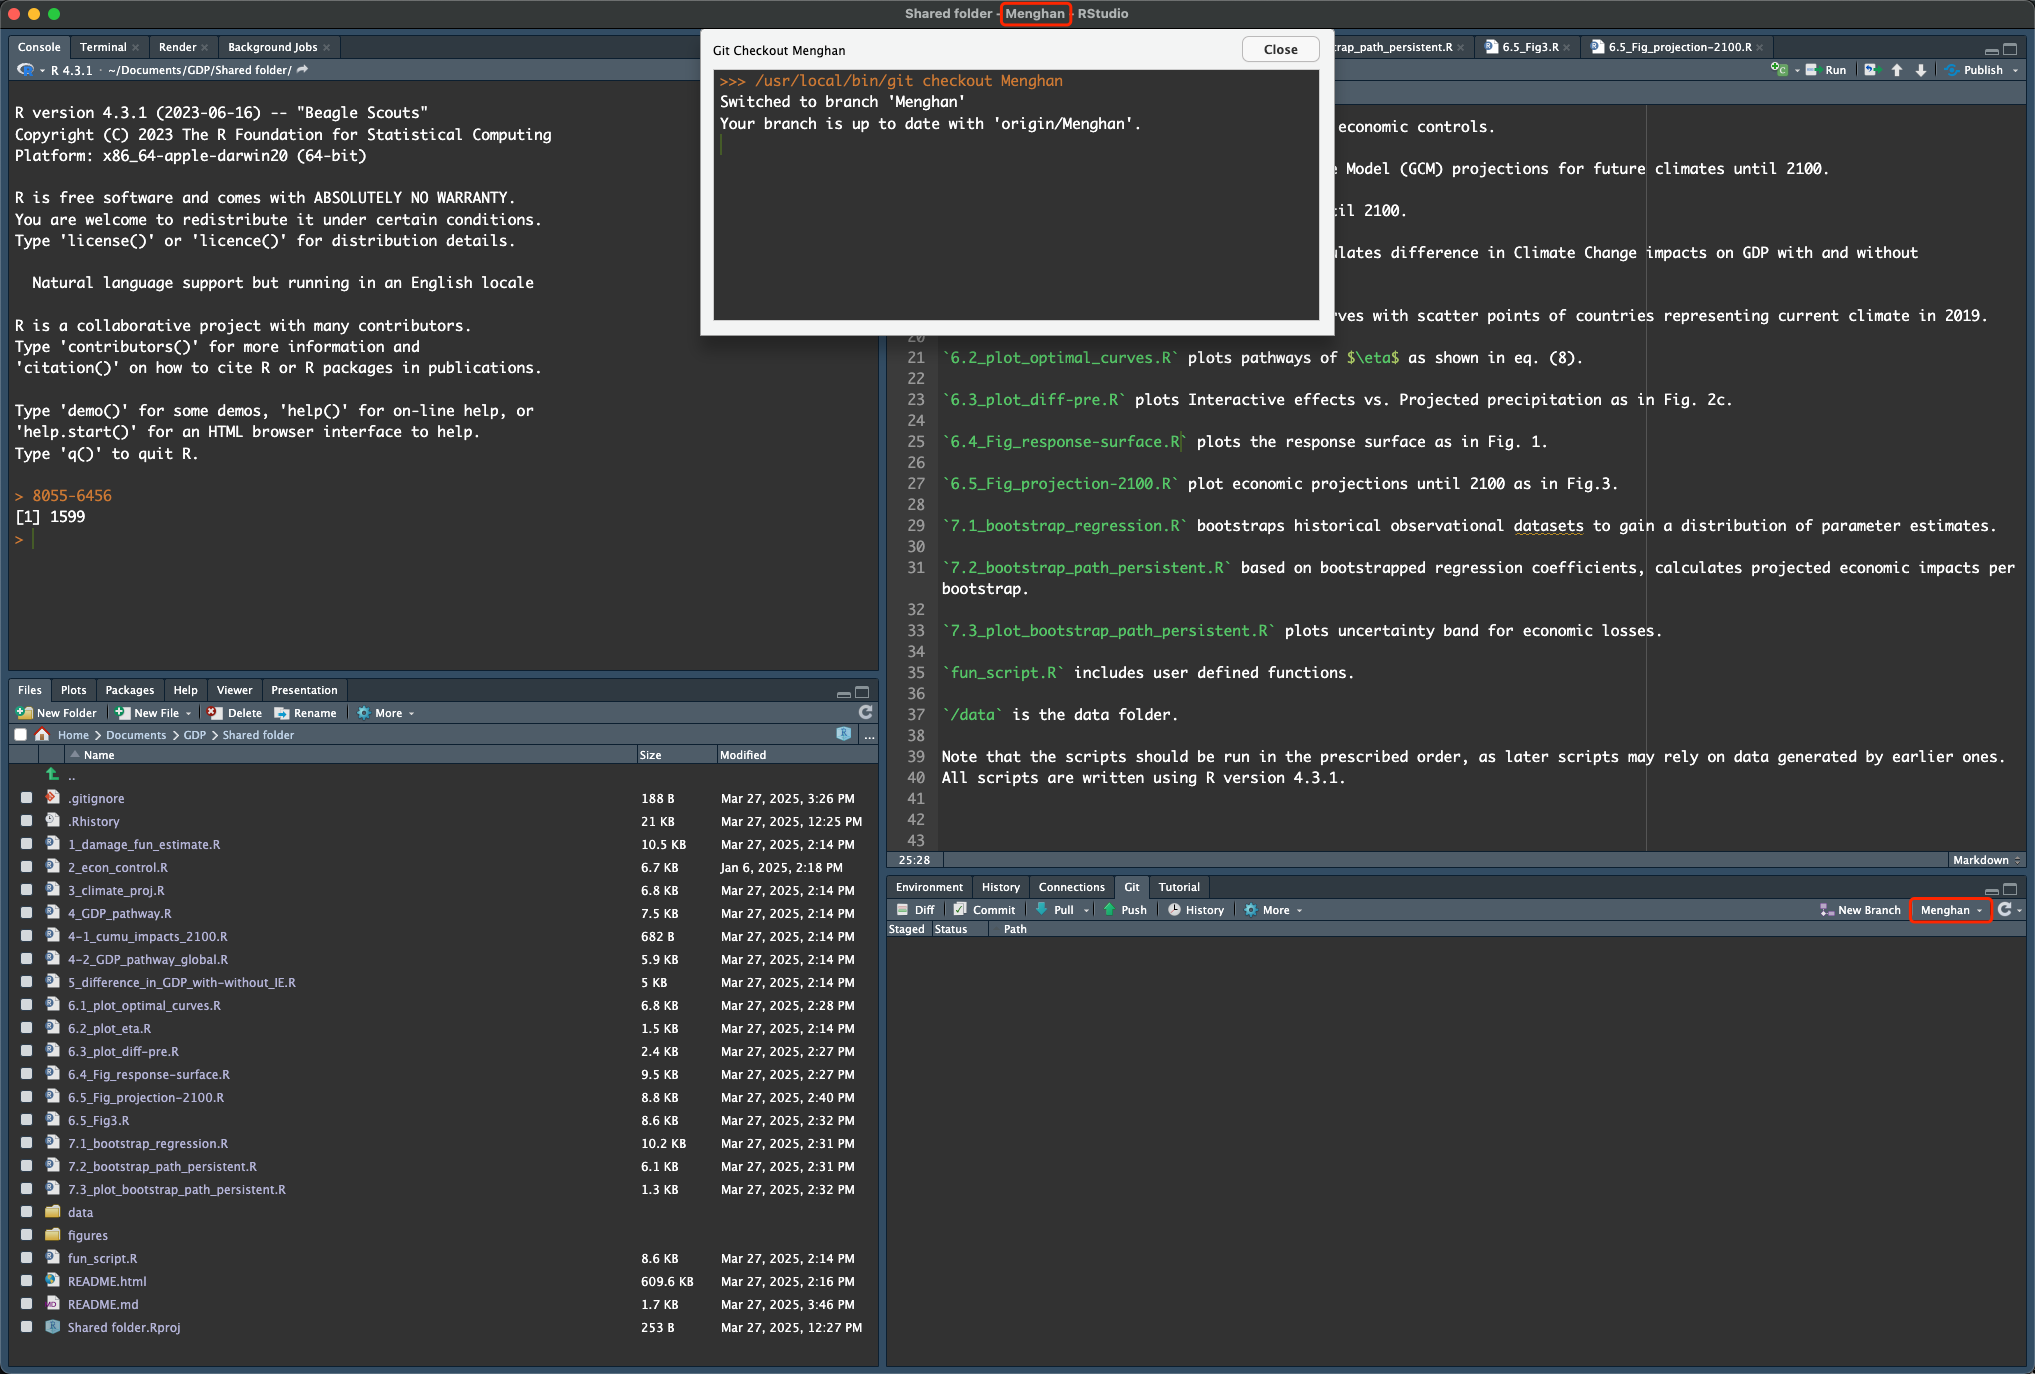
\includegraphics[width=1\linewidth]{images/R git branch}

Choose a License for your repo

Q: Which open source license is appropriate for my project?\\
A: See \url{https://opensource.guide/legal/\#which-open-source-license-is-appropriate-for-my-project}.

Q: How to add a license to my repo?\\
A: Follow the instructions \href{https://docs.github.com/en/communities/setting-up-your-project-for-healthy-contributions/adding-a-license-to-a-repository}{here}.

\begin{center}\rule{0.5\linewidth}{0.5pt}\end{center}

\section{Copilot}\label{copilot}

Copilot offers autocomplete-style suggestions as you code as ``ghost text''.

GitHub Copilot primarily relies on the context in the file you are actively editing. Any comments, code, or other context provided within the active document will be used as a ``prompt'' that Copilot will then use to provide a suggested completion.

\begin{itemize}
\item
  To expand the scope of the context used by Copilot beyond just the active document, there is a setting to also index and read from other R, Python, or SQL files in the current project. This setting can be toggled on or off in the Tools \textgreater{} Global Options \textgreater{} Copilot \textgreater{} ``Index project files with GitHub Copilot'' setting.
\item
  At times, normal autocomplete and Copilot may seem to conflict with each other. In these cases, it is best to review the Copilot suggestion and determine if it is appropriate for the current context. If it is, you can accept the suggestion by pressing \texttt{Tab}. If it is not, you can ignore the suggestion and continue typing or force the normal autocomplete to show by pressing \texttt{Ctrl+Space}.

  Issue: \texttt{Ctrl+Space} crash with spotlight shortcut. ❗️
\item
  Only show Copilot suggestions when evoke mannually using \texttt{Ctrl\ +\ Backslash\ (\textbackslash{})}.

  The Copilot suggestions can be very distracting and clutter your script.
\end{itemize}

For general advice on how to use Copilot, please see:

\begin{itemize}
\tightlist
\item
  \href{https://docs.posit.co/ide/user/ide/guide/tools/copilot.html}{RStudio Copilot User Guide}
\item
  \href{https://github.blog/2023-06-20-how-to-write-better-prompts-for-github-copilot/}{How to use GitHub Copilot: Prompts, tips, and use cases}
\end{itemize}

\begin{center}\rule{0.5\linewidth}{0.5pt}\end{center}

\section{Save R Workspace}\label{save-r-workspace}

If you want to saves {all objects} in your work space, use \texttt{save.image()}. It will creates an image of your current variables and functions, and saves them to a file called \texttt{.RData}. When R next loads, objects stored in this image are by default restored.

This sounds convenient, however, you do NOT want to do this because this corrupt {reproducibility} of your project. ❌

You want to {start from a clean slate} very time. ✅

It is suggested change RStudio Global Options to

\begin{itemize}
\tightlist
\item
  \emph{not} ``restore \texttt{.RData} into workspace at startup'', and
\item
  \emph{never} ``save workspace to \texttt{.RData} on exit''.
\end{itemize}

In case you do feel the need to save the workspace, use the following cmd.

\texttt{save.image(file\ =\ ".RData",\ version\ =\ NULL,\ ascii\ =\ FALSE,\ compress\ =\ !ascii,\ safe\ =\ TRUE)}

\begin{Shaded}
\begin{Highlighting}[]
\DocumentationTok{\#\# save current workspace \#\#}
\NormalTok{f\_name }\OtherTok{\textless{}{-}} \StringTok{"RImage/TCR\_2023{-}05{-}09.RData"}
\NormalTok{f\_name}
\FunctionTok{save.image}\NormalTok{(f\_name)}
\CommentTok{\# load(f\_name)}
\end{Highlighting}
\end{Shaded}

Q: Can I save the loaded packages in the current session/workspace?\\
A: The workspace is for \emph{objects} like data and functions. Starting R with particular packages loaded is what your \texttt{.Rprofile} file is for, and you can have a different one in each directory. But I'd recommend not saving anything between r sessions and instead recreate it all using code. This is much more likely to lead to reproducible results.

\textbf{History}

When you quit a project, \texttt{.Rhistory} is automatically written to the project directory unless you opt out to. It contains a history of all of the commands that you have sent to the R console in this session.

\begin{center}\rule{0.5\linewidth}{0.5pt}\end{center}

\textbf{Pop out an editor}

Click the \texttt{Show\ in\ New\ Window} button in any source editor tab.

To return a document to the main window, click the \texttt{Return\ to\ Main\ Window} button on the editor toolbar.

\begin{center}\rule{0.5\linewidth}{0.5pt}\end{center}

\textbf{Environment Pane}

By default, the Environment pane is located in the top-right and includes the Environment, History, Connections, Build, and Version Control System (VCS) tabs.

Version Control System (VCS)

The VCS tab will change based on the version control system you have enabled for that session. For example, using Git will change the tab name to Git and provide some common commands for viewing diffs, committing changes, pull and push \ldots{}
Output pane

The Output pane displays various outputs such as plots, HTML content, or on-disk files. It contains the Files, Plots, R Packages, Help, Viewer, and Presentation tabs.

Ref: \href{https://docs.posit.co/ide/user/ide/guide/ui/ui-panes.html\#:~:text=four\%20primary\%20panes.-,To\%20add\%20additional\%20source\%20columns\%2C\%20from\%20the\%20RStudio\%20menu\%3A\%20Global,only\%20within\%20the\%20Source\%20pane.}{RStudio Pane Layout}

\begin{center}\rule{0.5\linewidth}{0.5pt}\end{center}

\textbf{Global Options that make coding easier}

\begin{itemize}
\item
  Syntax highlight and matched parentheses.

  Under ``Tools -\textgreater{} Global Options -\textgreater{} Code -\textgreater{} Display'', under \textbf{Syntax section}, check the boxes for \textbf{highlight R function calls} and \textbf{use rainbow parentheses}. The second is especially useful to mark matching opening and closing brackets.
\item
  Show whitespace characters.

  In ``Tools -\textgreater{} Global Options -\textgreater{} Code -\textgreater{} Display'', check ``Show whitespace characters''. This will let you see spaces and newlines in the editor.
\end{itemize}

References:

\url{https://coding-club.rostools.org/posts/tips-and-tricks/}

\begin{center}\rule{0.5\linewidth}{0.5pt}\end{center}

\section{Options}\label{options}

\textbf{\texttt{getOption(x)}} Allow the user to set and examine a variety of global \emph{options} which affect the way in which \textbf{R computes and displays its results.} Use \texttt{getOption} to check default values of global options.

\begin{itemize}
\tightlist
\item
  \texttt{x} a {character string }holding an option name, must be {quoted in quotes}
\item
  Can only query one option at a time. If multiple options are given, will return the value of the first option.
\end{itemize}

\textbf{\texttt{options(...)}} query and modify global options.

\begin{itemize}
\item
  \texttt{...} any options can be defined, using \texttt{name\ =\ value}.

  Note that you do {NOT need to quote your option name} here!
\item
  \texttt{options()} with no arguments returns a list with the current values of the options.
\item
  \texttt{options("name")} can be used to examine options' current value too; return a \emph{list}, whereas \texttt{getOption("name")} returns the value only.

  \begin{itemize}
  \item
    Note that you need to quote the option name when you do queries.
  \item
    You can query more than one options at a time.

\begin{Shaded}
\begin{Highlighting}[]
\SpecialCharTok{\textgreater{}} \FunctionTok{options}\NormalTok{(}\StringTok{"width"}\NormalTok{, }\StringTok{"digits"}\NormalTok{)}
\SpecialCharTok{$}\NormalTok{width}
\NormalTok{[}\DecValTok{1}\NormalTok{] }\DecValTok{90}

\SpecialCharTok{$}\NormalTok{digits}
\NormalTok{[}\DecValTok{1}\NormalTok{] }\DecValTok{7}

\SpecialCharTok{\textgreater{}} \FunctionTok{getOption}\NormalTok{(}\StringTok{"width"}\NormalTok{, }\StringTok{"digits"}\NormalTok{)}
\NormalTok{[}\DecValTok{1}\NormalTok{] }\DecValTok{90}
\end{Highlighting}
\end{Shaded}
  \end{itemize}
\end{itemize}

\textbf{\texttt{?options}} to get the help page of global options. To check which options are available and their definitions.

\textbf{Use examples}

\begin{Shaded}
\begin{Highlighting}[]
\DocumentationTok{\#\# Two ways checking default option values}
\SpecialCharTok{\textgreater{}} \FunctionTok{options}\NormalTok{(}\StringTok{"width"}\NormalTok{)}
\SpecialCharTok{$}\NormalTok{width}
\NormalTok{[}\DecValTok{1}\NormalTok{] }\DecValTok{81}

\SpecialCharTok{\textgreater{}} \FunctionTok{getOption}\NormalTok{(}\StringTok{"width"}\NormalTok{)}
\NormalTok{[}\DecValTok{1}\NormalTok{] }\DecValTok{81}

\DocumentationTok{\#\# Change option values}
\CommentTok{\# use name=value}
\SpecialCharTok{\textgreater{}} \FunctionTok{options}\NormalTok{(}\AttributeTok{width=}\DecValTok{80}\NormalTok{, }\AttributeTok{digits=}\DecValTok{15}\NormalTok{) }\CommentTok{\# set print width, digits to print for numeric values using name=value paris}
\CommentTok{\# use a named list}
\SpecialCharTok{\textgreater{}} \FunctionTok{options}\NormalTok{(}\FunctionTok{list}\NormalTok{(}\AttributeTok{width=}\DecValTok{80}\NormalTok{, }\AttributeTok{digits=}\DecValTok{15}\NormalTok{)) }
\end{Highlighting}
\end{Shaded}

\textbf{Commonly used global options}:

\begin{longtable}[]{@{}
  >{\raggedright\arraybackslash}p{(\linewidth - 2\tabcolsep) * \real{0.1781}}
  >{\raggedright\arraybackslash}p{(\linewidth - 2\tabcolsep) * \real{0.8219}}@{}}
\toprule\noalign{}
\begin{minipage}[b]{\linewidth}\raggedright
Option
\end{minipage} & \begin{minipage}[b]{\linewidth}\raggedright
Description
\end{minipage} \\
\midrule\noalign{}
\endhead
\bottomrule\noalign{}
\endlastfoot
width & Controls the maximum number of columns on a line used in printing vectors, matrices and arrays, and when filling by \texttt{cat}. Defaults to 80.Don't change this if you want to print more columns. Use {\texttt{options(tibble.width=400)}} instead. \\
pillar.sigfig & Tibbles print numbers with three significant digits by default, switching to scientific notation if the available space is too small.\texttt{options(pillar.sigfig\ =\ 4)} to increase the number of digits printed out \\
\end{longtable}

\begin{center}\rule{0.5\linewidth}{0.5pt}\end{center}

\section{R Startup}\label{r-startup}

\textbf{\texttt{Sys.getenv(x)}} get the values of the environment variables. Returns a vector of the same length as \texttt{x}.

\begin{itemize}
\tightlist
\item
  \texttt{x} a character vector
\end{itemize}

Environment Variables examples:

\begin{Shaded}
\begin{Highlighting}[]
\SpecialCharTok{\textgreater{}} \FunctionTok{Sys.getenv}\NormalTok{(}\FunctionTok{c}\NormalTok{(}\StringTok{"HOME"}\NormalTok{, }\StringTok{"R\_HOME"}\NormalTok{, }\StringTok{"R\_PAPERSIZE"}\NormalTok{, }\StringTok{"R\_PRINTCMD"}\NormalTok{))}
\NormalTok{           HOME                                      R\_HOME }
\StringTok{"/Users/menghan"} \StringTok{"/Library/Frameworks/R.framework/Resources"} 
\NormalTok{    R\_PAPERSIZE                                  R\_PRINTCMD }
           \StringTok{"a4"}                                       \StringTok{"lpr"} 
\end{Highlighting}
\end{Shaded}

\href{https://community.rstudio.com/t/rstudio-doesnnt-load-rprofile-or-renviron/57721}{Rstudio doesnn't load Rprofile or Renviron}

I store my \texttt{Rprofile} and \texttt{Renviron} in non-default places (i.e.~\texttt{\textasciitilde{}/.config/R}). When opening \texttt{R} in a normal shell, my environment is loaded perfectly fine. When opening Rstudio, it doesn't load my options, settings or paths.

\begin{itemize}
\item
  Have to {wrap your option settings in \texttt{rstudio.sessionInit}}

  \url{https://damien-datasci-blog.netlify.app/post/2020-12-31-pimp-your-r-startup-message/}

  \begin{itemize}
  \item
    Open \texttt{.Rprofile}

\begin{Shaded}
\begin{Highlighting}[]
\NormalTok{usethis}\SpecialCharTok{::}\FunctionTok{edit\_r\_profile}\NormalTok{()}
\end{Highlighting}
\end{Shaded}
  \item
    wrap up your options in the following snippet

\begin{Shaded}
\begin{Highlighting}[]
\FunctionTok{setHook}\NormalTok{(}\StringTok{"rstudio.sessionInit"}\NormalTok{, }\ControlFlowTok{function}\NormalTok{(newSession) \{}
  \CommentTok{\# any code included here will be run at the start of each RStudio session}
  \FunctionTok{options}\NormalTok{(}\AttributeTok{buildtools.check =} \ControlFlowTok{function}\NormalTok{(action) }\ConstantTok{TRUE}\NormalTok{ )}
\NormalTok{\}, }\AttributeTok{action =} \StringTok{"append"}\NormalTok{)}
\end{Highlighting}
\end{Shaded}
  \end{itemize}
\item
  Understanding R's startup

  \url{https://rviews.rstudio.com/2017/04/19/r-for-enterprise-understanding-r-s-startup/}
\end{itemize}

\href{https://usethis.r-lib.org/reference/index.html}{\texttt{usethis}} is a workflow package: it automates repetitive tasks that arise during project setup and development, both for R packages and non-package projects.

What is \texttt{.Rprofile}?

\texttt{.Rprofile} is a startup file to set options and environment variables. \texttt{.Rprofile} files can be either at the user or project level.

\begin{itemize}
\tightlist
\item
  User-level \texttt{.Rprofile} files live in the base of the user's {home directory}, and
\item
  project-level \texttt{.Rprofile} files live in the base of the project directory.
\end{itemize}

Quitting R will erase the default theme setting. If you load \texttt{ggplot2} in a future session it will revert to the default gray theme. If you'd like for \texttt{ggplot2} to always use a different theme (either yours or one of the built-in ones), you can set a load hook and put it in your \texttt{.Rprofile} file. For example, the following hook sets the default theme to be \texttt{theme\_minimal()} every time the \texttt{ggplot2} package is loaded.

\begin{Shaded}
\begin{Highlighting}[]
\FunctionTok{setHook}\NormalTok{(}\FunctionTok{packageEvent}\NormalTok{(}\StringTok{"ggplot2"}\NormalTok{, }\StringTok{"onLoad"}\NormalTok{), }
        \ControlFlowTok{function}\NormalTok{(...) ggplot2}\SpecialCharTok{::}\FunctionTok{theme\_set}\NormalTok{(ggplot2}\SpecialCharTok{::}\FunctionTok{theme\_bw}\NormalTok{()))}
\end{Highlighting}
\end{Shaded}

Of course, you can always override this default theme by adding a theme object to any of your plots that you construct in \texttt{ggplot2}.

\href{https://community.rstudio.com/t/rcpp-compilation-breaks-in-r-4-1-0-running-on-big-sur-11-4/109744}{Rcpp compilation breaks in R 4.1.0}

\begin{Shaded}
\begin{Highlighting}[]
\NormalTok{devtools}\SpecialCharTok{::}\FunctionTok{build}\NormalTok{(}\StringTok{"my\_package"}\NormalTok{)}
\NormalTok{Error}\SpecialCharTok{:}\NormalTok{ Could not find tools necessary to compile a package}
\NormalTok{Call }\StringTok{\textasciigrave{}}\AttributeTok{pkgbuild::check\_build\_tools(debug = TRUE)}\StringTok{\textasciigrave{}}\NormalTok{ to diagnose the problem.}
\end{Highlighting}
\end{Shaded}

\begin{itemize}
\item
  In RStudio, I am continually prompted to install additional build tools and I can't install the build tool. \(\rightarrow\) Bypass the option \texttt{options(buildtools.check\ =\ function(action)\ TRUE)}.
\item
  Turns out R was pointing to an old clang version in my Makevars.

  I just deleted it using {[}in Terminal{]}

\begin{Shaded}
\begin{Highlighting}[]
\FunctionTok{sudo}\NormalTok{ rm \textasciitilde{}/.R/Makevars}
\end{Highlighting}
\end{Shaded}
\end{itemize}

\textbf{Install SDK command line tool}

Download from developer.apple.com. Software development kit.

\url{https://developer.apple.com/download/all/}

\textbf{R compiler tools for cpp on MacOS}

\begin{itemize}
\item
  \url{https://thecoatlessprofessor.com/programming/cpp/r-compiler-tools-for-rcpp-on-macos/}
\item
  install OpenMP enabled \texttt{clang} from the terminal

  \url{https://rpubs.com/Kibalnikov/776164}
\end{itemize}

\chapter{Knit Rmd}\label{knit-rmd}

\textbf{R Markdown} is a powerful tool for combining analysis and reporting into the same document. R Markdown has grown substantially from a package that supports a few output formats, to an extensive and diverse ecosystem that supports the creation of books, blogs, scientific articles, websites, and even resumes.

Nice documentations

\begin{itemize}
\tightlist
\item
  \textbf{\texttt{rmarkdown}} package CRAN

  \begin{itemize}
  \tightlist
  \item
    \href{https://cran.r-project.org/web/packages/rmarkdown/index.html}{Package CRAN page}
  \item
    \href{https://cran.r-project.org/web/packages/rmarkdown/rmarkdown.pdf}{Reference manual}
  \end{itemize}
\item
  \textbf{\texttt{bookdown}} package CRAN

  \begin{itemize}
  \tightlist
  \item
    \href{https://cran.r-project.org/web/packages/bookdown/index.html}{Package CRAN page}
  \item
    \href{https://cran.r-project.org/web/packages/bookdown/bookdown.pdf}{Reference manual}
  \end{itemize}
\item
  \href{https://bookdown.org/yihui/rmarkdown}{R markdown: The definitive guide.} provides detailed references
\item
  \href{https://bookdown.org/yihui/rmarkdown-cookbook/}{R markdown cookbook}: concise and covers essential functions, with examples.
\item
  \href{https://bookdown.org/yihui/bookdown/}{Authoring Books with R Markdown}: with a focus on \texttt{bookdown}.
\end{itemize}

Q: What is the difference between Rmd and R script?\\
A:

\begin{itemize}
\tightlist
\item
  An R script (\texttt{.R}) is used for developing and troubleshooting code; a place where you can store reusable code fragments.
\item
  An R Markdown file (\texttt{.Rmd}) is used to integrate R commands with explanatory text and output, making it useful for creating reports.
\end{itemize}

\begin{center}\rule{0.5\linewidth}{0.5pt}\end{center}

\textbf{Quick takeaways}:

\begin{itemize}
\tightlist
\item
  Can still use horizontal separator \texttt{ctrl\ +\ shift\ +\ S} for dashed lines and \texttt{ctrl\ +\ shift\ +\ =} for equals
\item
  Headers must have one empty line above and below to separate it from other text
\end{itemize}

\begin{center}\rule{0.5\linewidth}{0.5pt}\end{center}

YAML metadata

Q: What is YAML?\\
A: YAML is a human-friendly data serialization language for all programming languages. YAML stands for ``Yet Another Markup Language.''

Q: What does YAML do?\\
A: It is placed at the very beginning of the document and is read by each of Pandoc, \textbf{rmarkdown}, and \textbf{knitr}.

\begin{itemize}
\tightlist
\item
  Provide metadata of the document.
\item
  located at the top of the file.
\item
  adheres to the YAML format and is delimited by lines containing three three dashes (\texttt{-\/-\/-}).
\end{itemize}

YAML also called header and front matter.

See \href{https://github.com/hao203/rmarkdown-YAML.git}{HERE} for commonly used YAML metadata (header) in different R Markdown output formats.

YAML can set values of the template variables, such as \texttt{title}, \texttt{author}, and \texttt{date} of the document.

\begin{itemize}
\item
  The \texttt{output} field is used by rmarkdown to apply the {\textbf{output format function}} \texttt{rmarkdown::html\_document()} in the rendering process.

  There are two types of output formats in the \textbf{rmarkdown} package: documents (e.g., \texttt{pdf\_document}), and presentations (e.g., \texttt{beamer\_presentation}).

  Supported output format examples: \texttt{html\_document}, \texttt{pdf\_document}.

  R Markdown documents (\texttt{html\_documents}) and R Notebook documents (\texttt{html\_notebook}) are very similar; in fact, an R Notebook document is a special type of R Markdown document. The main difference is using R Markdown document (\texttt{html\_documents}) you have to knit (render) the entire document each time you want to preview the document, even if you have made a minor change. However, using an R Notebook document (\texttt{html\_notebook}) you can view a preview of the final document without rendering the entire document.

  \textbf{Troubleshooting}

  Issue: \texttt{bookdown} always output html, even if specified to pdf.\\
  Cause: If it produces HTML, the output format must have been provided somewhere.\\
  Fix: Check if you have a \texttt{\_output.yml} under the root directory of your book project. If you do, you may delete it. Then bookdown will use the output field that you specified in the YAML frontmatter of your Rmd document.

  If there are two output formats, \texttt{rmarkdown::render()} defaults to use the first output type. If you want another, specify the type, e.g., \texttt{rmarkdown::render("0100-RStudio.Rmd",\ \textquotesingle{}pdf\_document\textquotesingle{})}.
\end{itemize}

\begin{center}\rule{0.5\linewidth}{0.5pt}\end{center}

\textbf{\texttt{bookdown} wrappers} of base markdown format

{\texttt{bookdown} output formats} allow numbering and cross-referencing figures/tables/equations. It takes the format \texttt{html\_document2}, in general, \texttt{markdown\_document2} is a wrapper for the base format \texttt{markdown\_document}. With the \texttt{bookdown} output format, you can cross-reference sections by their ID's using the same syntax when sections are numbered.

Other bookdown output format examples for single documents: \texttt{pdf\_document2}, \texttt{beamer\_presentation2}, \texttt{tufte\_html2}, \texttt{word\_document2}. See Page 12 of the \href{https://cran.r-project.org/web/packages/bookdown/bookdown.pdf}{reference manual} for a complete list of supported format by \texttt{bookdown}.

What bookdown is very powerful for is that it compiles books. Book formats:

\begin{itemize}
\tightlist
\item
  HTML:

  \begin{itemize}
  \tightlist
  \item
    \texttt{gitbook}
  \item
    \texttt{html\_book}
  \item
    \texttt{tufte\_html\_book}
  \end{itemize}
\item
  PDF:

  \begin{itemize}
  \tightlist
  \item
    \texttt{pdf\_book}
  \end{itemize}
\item
  e-book:

  \begin{itemize}
  \tightlist
  \item
    \texttt{epub\_book}
  \end{itemize}
\end{itemize}

\begin{center}\rule{0.5\linewidth}{0.5pt}\end{center}

\begin{itemize}
\item
  Many aspects of the LaTeX template used to create PDF documents can be customized using {\textbf{top-level}} \href{https://bookdown.org/yihui/rmarkdown/pdf-document.html\#tab:latex-vars}{YAML metadata} (note that these options do {\textbf{NOT}} appear underneath the \texttt{output} section, but rather appear at the top level along with \texttt{title}, \texttt{author}, and so on). For example:

\begin{Shaded}
\begin{Highlighting}[]
\CommentTok{{-}{-}{-}}
\AnnotationTok{title:}\CommentTok{ "Crop Analysis Q3 2013"}
\AnnotationTok{output:}\CommentTok{ pdf\_document}
\AnnotationTok{fontsize:}\CommentTok{ 11pt}
\AnnotationTok{geometry:}\CommentTok{ margin=1in}
\CommentTok{{-}{-}{-}}
\end{Highlighting}
\end{Shaded}

  A few available metadata variables are displayed in the following (consult the Pandoc manual for \href{https://pandoc.org/MANUAL.html\#variables-for-latex}{the full list}):

  \begin{longtable}[]{@{}
    >{\raggedright\arraybackslash}p{(\linewidth - 2\tabcolsep) * \real{0.4340}}
    >{\raggedright\arraybackslash}p{(\linewidth - 2\tabcolsep) * \real{0.5660}}@{}}
  \toprule\noalign{}
  \begin{minipage}[b]{\linewidth}\raggedright
  Top-level YAML Variable
  \end{minipage} & \begin{minipage}[b]{\linewidth}\raggedright
  Description
  \end{minipage} \\
  \midrule\noalign{}
  \endhead
  \bottomrule\noalign{}
  \endlastfoot
  \texttt{lang} & Document language code \\
  \texttt{fontsize} & Font size (e.g., \texttt{10pt}, \texttt{11pt}, or \texttt{12pt}) \\
  \texttt{papersize} & Defines the paper size (e.g., \texttt{a4paper}, \texttt{letterpaper}) \\
  \texttt{documentclass} & LaTeX document class (e.g., \texttt{article}, \texttt{book}, and \texttt{report}) \\
  \texttt{classoption} & A list of options to be passed to the document class, e.g., you can create a two-column document with the \texttt{twocolumn} option. \\
  \texttt{geometry} & Options for \href{https://ctan.org/pkg/geometry}{\texttt{geometry}} package (e.g., \texttt{margin=1in} set all margins to be 1 inch) \\
  \texttt{mainfont}, \texttt{sansfont}, \texttt{monofont}, \texttt{mathfont} & Document fonts (works only with \texttt{xelatex} and \texttt{lualatex}) \\
  \texttt{linkcolor}, \texttt{urlcolor}, \texttt{citecolor} & Color for internal links (cross references), external links (link to websites), and citation links (bibliography) \\
  \texttt{linestretch} & Options for line spacing (e.g.~1, 1.5, 3). \\
  \end{longtable}

  Pandoc User's Guide: \url{https://www.uv.es/wiki/pandoc_manual_2.7.3.wiki?21}

  \texttt{classoption}

  \begin{itemize}
  \item
    \textbf{\texttt{onecolumn}, \texttt{twocolumn}} - Instructs LaTeX to typeset the document in one column or two columns.
  \item
    \textbf{\texttt{twoside}, \texttt{oneside}}: Specifies whether double or single sided output should be generated. The classes' article and report are single sided and the book class is double sided by default.

    Note that this option concerns the style of the document only. The option two side does \emph{NOT} tell the printer you use that it should actually make a two-sided printout.

    The difference between single-sided and double-sided documents in LaTeX lies in the layout of the page margins and the orientation of the text on the page.

    \begin{itemize}
    \item
      Single-sided documents are printed on only one side of the page, with the text and images aligned to the right-hand side of the page. This type of layout is often used for brochures, flyers, and other types of promotional materials.
    \item
      Double-sided documents are printed on both sides of the page, with the text and images alternating between right-hand and left-hand margins. This type of layout is often used for \textbf{books}, reports, and other types of long-form documents.

      A \texttt{twoside} document has different margins and headers/footers for odd and even pages.
    \end{itemize}

    The layout of a \texttt{twoside} book

    Q: Why Inner margin is narrow?\\
    A: The reason for this is that with two pages side by side, you actually have only THREE margins - the left, right and middle. The middle margin is made up from the inside margins of both pages, and so these are smaller because they add together to make the middle margin. If they were bigger, then you would end up with too much whitespace in the middle.

\begin{Shaded}
\begin{Highlighting}[]
\NormalTok{o }\SpecialCharTok{{-}}\NormalTok{ outside margin}
\NormalTok{i }\SpecialCharTok{{-}}\NormalTok{ inside margin}
\NormalTok{b }\SpecialCharTok{{-}}\NormalTok{ binding offset}

\NormalTok{Before binding}\SpecialCharTok{:}
\SpecialCharTok{{-}{-}{-}{-}{-}{-}{-}{-}{-}{-}{-}{-}{-}{-}{-}{-}{-}{-}}    \SpecialCharTok{{-}{-}{-}{-}{-}{-}{-}{-}{-}{-}{-}{-}{-}{-}{-}{-}{-}}
\ErrorTok{|}\NormalTok{oooo}\SpecialCharTok{|}\ErrorTok{\textasciitilde{}\textasciitilde{}\textasciitilde{}\textasciitilde{}\textasciitilde{}\textasciitilde{}|}\NormalTok{ii}\SpecialCharTok{|}\NormalTok{b}\SpecialCharTok{|}    \ErrorTok{|} \ErrorTok{|}  \ErrorTok{|\textasciitilde{}\textasciitilde{}\textasciitilde{}\textasciitilde{}\textasciitilde{}\textasciitilde{}|}   \ErrorTok{|}
\ErrorTok{|}    \ErrorTok{|\textasciitilde{}\textasciitilde{}\textasciitilde{}\textasciitilde{}\textasciitilde{}\textasciitilde{}|}  \ErrorTok{|} \ErrorTok{|}    \ErrorTok{|} \ErrorTok{|}  \ErrorTok{|\textasciitilde{}\textasciitilde{}\textasciitilde{}\textasciitilde{}\textasciitilde{}\textasciitilde{}|}   \ErrorTok{|}
\ErrorTok{|}    \ErrorTok{|\textasciitilde{}\textasciitilde{}\textasciitilde{}\textasciitilde{}\textasciitilde{}\textasciitilde{}|}  \ErrorTok{|} \ErrorTok{|}    \ErrorTok{|} \ErrorTok{|}  \ErrorTok{|\textasciitilde{}\textasciitilde{}\textasciitilde{}\textasciitilde{}\textasciitilde{}\textasciitilde{}|}   \ErrorTok{|}
\ErrorTok{|}    \ErrorTok{|\textasciitilde{}\textasciitilde{}\textasciitilde{}\textasciitilde{}\textasciitilde{}\textasciitilde{}|}  \ErrorTok{|} \ErrorTok{|}    \ErrorTok{|} \ErrorTok{|}  \ErrorTok{|\textasciitilde{}\textasciitilde{}\textasciitilde{}\textasciitilde{}\textasciitilde{}\textasciitilde{}|}   \ErrorTok{|}
\ErrorTok{|}    \ErrorTok{|\textasciitilde{}\textasciitilde{}\textasciitilde{}\textasciitilde{}\textasciitilde{}\textasciitilde{}|}  \ErrorTok{|} \ErrorTok{|}    \ErrorTok{|} \ErrorTok{|}  \ErrorTok{|\textasciitilde{}\textasciitilde{}\textasciitilde{}\textasciitilde{}\textasciitilde{}\textasciitilde{}|}   \ErrorTok{|}
\ErrorTok{|}    \ErrorTok{|\textasciitilde{}\textasciitilde{}\textasciitilde{}\textasciitilde{}\textasciitilde{}\textasciitilde{}|}  \ErrorTok{|} \ErrorTok{|}    \ErrorTok{|} \ErrorTok{|}  \ErrorTok{|\textasciitilde{}\textasciitilde{}\textasciitilde{}\textasciitilde{}\textasciitilde{}\textasciitilde{}|}   \ErrorTok{|}
\SpecialCharTok{{-}{-}{-}{-}{-}{-}{-}{-}{-}{-}{-}{-}{-}{-}{-}{-}{-}{-}}    \SpecialCharTok{{-}{-}{-}{-}{-}{-}{-}{-}{-}{-}{-}{-}{-}{-}{-}{-}{-}}

\NormalTok{After binding}\SpecialCharTok{:}
\SpecialCharTok{{-}{-}{-}{-}{-}{-}{-}{-}{-}{-}{-}{-}{-}{-}{-}{-}{-}{-}{-}{-}{-}{-}{-}{-}{-}{-}{-}{-}{-}{-}{-}}
\ErrorTok{|}\NormalTok{oooo}\SpecialCharTok{|}\ErrorTok{\textasciitilde{}\textasciitilde{}\textasciitilde{}\textasciitilde{}\textasciitilde{}\textasciitilde{}|}\NormalTok{ii}\SpecialCharTok{|}\NormalTok{ii}\SpecialCharTok{|}\ErrorTok{\textasciitilde{}\textasciitilde{}\textasciitilde{}\textasciitilde{}\textasciitilde{}\textasciitilde{}|}\NormalTok{oooo}\SpecialCharTok{|}
\ErrorTok{|}\NormalTok{oooo}\SpecialCharTok{|}\ErrorTok{\textasciitilde{}\textasciitilde{}\textasciitilde{}\textasciitilde{}\textasciitilde{}\textasciitilde{}|}\NormalTok{ii}\SpecialCharTok{|}\NormalTok{ii}\SpecialCharTok{|}\ErrorTok{\textasciitilde{}\textasciitilde{}\textasciitilde{}\textasciitilde{}\textasciitilde{}\textasciitilde{}|}\NormalTok{oooo}\SpecialCharTok{|}
\ErrorTok{|}\NormalTok{oooo}\SpecialCharTok{|}\ErrorTok{\textasciitilde{}\textasciitilde{}\textasciitilde{}\textasciitilde{}\textasciitilde{}\textasciitilde{}|}\NormalTok{ii}\SpecialCharTok{|}\NormalTok{ii}\SpecialCharTok{|}\ErrorTok{\textasciitilde{}\textasciitilde{}\textasciitilde{}\textasciitilde{}\textasciitilde{}\textasciitilde{}|}\NormalTok{oooo}\SpecialCharTok{|}
\ErrorTok{|}\NormalTok{oooo}\SpecialCharTok{|}\ErrorTok{\textasciitilde{}\textasciitilde{}\textasciitilde{}\textasciitilde{}\textasciitilde{}\textasciitilde{}|}\NormalTok{ii}\SpecialCharTok{|}\NormalTok{ii}\SpecialCharTok{|}\ErrorTok{\textasciitilde{}\textasciitilde{}\textasciitilde{}\textasciitilde{}\textasciitilde{}\textasciitilde{}|}\NormalTok{oooo}\SpecialCharTok{|}
\ErrorTok{|}\NormalTok{oooo}\SpecialCharTok{|}\ErrorTok{\textasciitilde{}\textasciitilde{}\textasciitilde{}\textasciitilde{}\textasciitilde{}\textasciitilde{}|}\NormalTok{ii}\SpecialCharTok{|}\NormalTok{ii}\SpecialCharTok{|}\ErrorTok{\textasciitilde{}\textasciitilde{}\textasciitilde{}\textasciitilde{}\textasciitilde{}\textasciitilde{}|}\NormalTok{oooo}\SpecialCharTok{|}
\ErrorTok{|}\NormalTok{oooo}\SpecialCharTok{|}\ErrorTok{\textasciitilde{}\textasciitilde{}\textasciitilde{}\textasciitilde{}\textasciitilde{}\textasciitilde{}|}\NormalTok{ii}\SpecialCharTok{|}\NormalTok{ii}\SpecialCharTok{|}\ErrorTok{\textasciitilde{}\textasciitilde{}\textasciitilde{}\textasciitilde{}\textasciitilde{}\textasciitilde{}|}\NormalTok{oooo}\SpecialCharTok{|}
\SpecialCharTok{{-}{-}{-}{-}{-}{-}{-}{-}{-}{-}{-}{-}{-}{-}{-}{-}{-}{-}{-}{-}{-}{-}{-}{-}{-}{-}{-}{-}{-}{-}{-}}
\end{Highlighting}
\end{Shaded}
  \item
    \textbf{\texttt{landscape}} - Changes the layout of the document to print in landscape mode.
  \item
    \textbf{\texttt{openright}, \texttt{openany}} - Makes chapters begin either only on right hand pages or on the next page available. This does not work with the article class, as it does not know about chapters. The report class by default starts chapters on the next page available and the book class starts them on right hand pages.
  \end{itemize}
\item
  In PDFs, you can use code, typesetting commands (e.g., \texttt{\textbackslash{}vspace\{12pt\}}), and specific packages from LaTeX.

  \begin{enumerate}
  \def\labelenumi{\arabic{enumi}.}
  \tightlist
  \item
    The \texttt{header-includes} option loads LaTeX packages.
  \end{enumerate}

\begin{Shaded}
\begin{Highlighting}[]
\CommentTok{{-}{-}{-}}
\AnnotationTok{output:}\CommentTok{ pdf\_document}
\AnnotationTok{header{-}includes:}
\CommentTok{  {-} \textbackslash{}usepackage\{fancyhdr\}}
\CommentTok{{-}{-}{-}}

\NormalTok{\textbackslash{}pagestyle\{fancy\}}
\NormalTok{\textbackslash{}fancyhead}\CommentTok{[}\OtherTok{LE,RO}\CommentTok{]}\NormalTok{\{Holly Zaharchuk\}}
\NormalTok{\textbackslash{}fancyhead}\CommentTok{[}\OtherTok{LO,RE}\CommentTok{]}\NormalTok{\{PSY 508\}}

\FunctionTok{\# Problem Set 12}
\end{Highlighting}
\end{Shaded}

  \href{https://github.com/hao203/rmarkdown-YAML?tab=readme-ov-file\#header-includes}{\textbf{Common \texttt{header-includes}:}}

  \begin{itemize}
  \tightlist
  \item
    Chinese/Japanese support
  \end{itemize}

\begin{Shaded}
\begin{Highlighting}[]
\CommentTok{{-}{-}{-}}
\AnnotationTok{output:}\CommentTok{ pdf\_document}
\AnnotationTok{header{-}includes:}
\CommentTok{  {-} \textbackslash{}usepackage\{ctex\}}
\CommentTok{{-}{-}{-}}
\end{Highlighting}
\end{Shaded}

  \begin{enumerate}
  \def\labelenumi{\arabic{enumi}.}
  \setcounter{enumi}{1}
  \tightlist
  \item
    Alternatively, use \texttt{extra\_dependencies} to list a character vector of LaTeX packages. This is useful if you need to load multiple packages:
  \end{enumerate}

\begin{Shaded}
\begin{Highlighting}[]
\CommentTok{{-}{-}{-}}
\AnnotationTok{title:}\CommentTok{ "Untitled"}
\AnnotationTok{output:}\CommentTok{ }
\CommentTok{  pdf\_document:}
\CommentTok{    extra\_dependencies: ["bbm", "threeparttable"]}
\CommentTok{{-}{-}{-}}
\end{Highlighting}
\end{Shaded}

  If you need to specify options when loading the package, you can add a second-level to the list and provide the options as a list:

\begin{Shaded}
\begin{Highlighting}[]
\CommentTok{{-}{-}{-}}
\AnnotationTok{title:}\CommentTok{ "Untitled"}
\AnnotationTok{output:}\CommentTok{ }
\CommentTok{  pdf\_document:}
\CommentTok{    extra\_dependencies:}
\CommentTok{      caption: ["labelfont=\{bf\}"]}
\CommentTok{      hyperref: ["unicode=true", "breaklinks=true"]}
\CommentTok{      lmodern: null}
\CommentTok{{-}{-}{-}}
\end{Highlighting}
\end{Shaded}

  Here are some examples of LaTeX packages you could consider using within your report:

  \begin{itemize}
  \tightlist
  \item
    \href{https://ctan.org/pkg/pdfpages}{pdfpages}: Include full PDF pages from an external PDF document within your document.
  \item
    \href{https://ctan.org/pkg/caption}{caption}: Change the appearance of caption subtitles. For example, you can make the figure title italic or bold.
  \item
    \href{https://ctan.org/pkg/fancyhdr}{fancyhdr}: Change the style of running headers of all pages.
  \end{itemize}
\item
  Some output options are passed to Pandoc, such as \texttt{toc}, \texttt{toc\_depth}, and \texttt{number\_sections}. You should consult the \href{https://pandoc.org/MANUAL.html\#variables}{Pandoc documentation} when in doubt.

\begin{Shaded}
\begin{Highlighting}[]
\CommentTok{{-}{-}{-}}
\AnnotationTok{output:}
\CommentTok{  pdf\_document:}
\CommentTok{    toc: true}
\CommentTok{    keep\_tex: true}
\CommentTok{{-}{-}{-}}
\end{Highlighting}
\end{Shaded}

  \begin{itemize}
  \tightlist
  \item
    \texttt{keep\_tex:\ true} if you want to keep intermediate TeX. Easy to debug. Defaults to \texttt{false}.
  \end{itemize}

  To learn which arguments a format takes, read the format's help page in R, e.g.~{\textbf{\texttt{?html\_document}}}.
\end{itemize}

\begin{center}\rule{0.5\linewidth}{0.5pt}\end{center}

\textbf{Parameters}

We can include variables and R expressions in this header that can be referenced throughout our R Markdown document. For example, the following header defines \texttt{start\_date} and \texttt{end\_date} parameters, which will be reflected in a list called \texttt{params} later in the R Markdown document.

\begin{Shaded}
\begin{Highlighting}[]
\CommentTok{{-}{-}{-}}
\AnnotationTok{title:}\CommentTok{ My RMarkdown}
\AnnotationTok{author:}\CommentTok{ Yihui Xie}
\AnnotationTok{output:}\CommentTok{ html\_document}
\AnnotationTok{params:}
\CommentTok{  start\_date: \textquotesingle{}2020{-}01{-}01\textquotesingle{}}
\CommentTok{  end\_date: \textquotesingle{}2020{-}06{-}01\textquotesingle{}}
\CommentTok{{-}{-}{-}}
\end{Highlighting}
\end{Shaded}

To access a parameter in our R code, call \texttt{params\$\textless{}parameter\ name\textgreater{}}, e.g., \texttt{params\$start\_date} and \texttt{params\$end\_date}.

Should I use quotes to surround the values?

\begin{itemize}
\tightlist
\item
  Whenever applicable use the unquoted style since it is the most readable.
\item
  Use quotes when the value can be misinterpreted as a data type or the value contains a \texttt{:}.
\end{itemize}

\begin{Shaded}
\begin{Highlighting}[]
\CommentTok{\# values need quotes}
\NormalTok{foo}\SpecialCharTok{:} \StringTok{\textquotesingle{}\{\{ bar \}\}\textquotesingle{}} \CommentTok{\# need quotes to avoid interpreting as \textasciigrave{}dict\textasciigrave{} object}
\NormalTok{foo}\SpecialCharTok{:} \StringTok{\textquotesingle{}123\textquotesingle{}}       \CommentTok{\# need quote to avoid interpreting as \textasciigrave{}int\textasciigrave{} object}
\NormalTok{foo}\SpecialCharTok{:} \StringTok{\textquotesingle{}yes\textquotesingle{}}           \CommentTok{\# avoid interpreting as \textasciigrave{}boolean\textasciigrave{} object}
\NormalTok{foo}\SpecialCharTok{:} \StringTok{"bar:baz:bam"} \CommentTok{\# has colon, can be misinterpreted as key}

\CommentTok{\# values need not quotes}
\NormalTok{foo}\SpecialCharTok{:}\NormalTok{ bar1baz234}
\NormalTok{bar}\SpecialCharTok{:} \DecValTok{123}\NormalTok{baz}
\end{Highlighting}
\end{Shaded}

ref:

\begin{itemize}
\tightlist
\item
  \href{https://bookdown.org/yihui/rmarkdown-cookbook/rmarkdown-anatomy.html\#:~:text=In\%20short\%2C\%20we\%20can\%20include\%20variables\%20and\%20R\%20expressions\%20in\%20this\%20header\%20that\%20can\%20be\%20referenced\%20throughout\%20our\%20R\%20Markdown\%20document.}{R Markdown anatomy, R Markdown Cookbook}
\item
  \url{https://rmarkdown.rstudio.com/lesson-6.html}
\end{itemize}

\begin{center}\rule{0.5\linewidth}{0.5pt}\end{center}

\subsection*{Compile an Rmd}\label{compile-an-rmd}

You can have more than output formats for your Rmd. For example, you want both the html and pdf output.

When you render the Rmd with \texttt{rmarkdown::render()}, it will use the \textbf{first output format you specify in the YAML metadata} (if it is missing, the default is \texttt{html\_document}).

do not want to use the first one, you can specify the one you want in the second argument, e.g., for an Rmd document \texttt{foo.Rmd} with the metadata:

\begin{Shaded}
\begin{Highlighting}[]
\FunctionTok{output}\KeywordTok{:}
\AttributeTok{  }\FunctionTok{html\_document}\KeywordTok{:}
\AttributeTok{    }\FunctionTok{toc}\KeywordTok{:}\AttributeTok{ }\CharTok{true}
\AttributeTok{  }\FunctionTok{pdf\_document}\KeywordTok{:}
\AttributeTok{    }\FunctionTok{keep\_tex}\KeywordTok{:}\AttributeTok{ }\CharTok{true}
\end{Highlighting}
\end{Shaded}

You can render it to PDF via:

\begin{Shaded}
\begin{Highlighting}[]
\NormalTok{rmarkdown}\SpecialCharTok{::}\FunctionTok{render}\NormalTok{(}\StringTok{\textquotesingle{}foo.Rmd\textquotesingle{}}\NormalTok{, }\StringTok{\textquotesingle{}pdf\_document\textquotesingle{}}\NormalTok{)}
\end{Highlighting}
\end{Shaded}

\begin{itemize}
\item
  RStudio calls the function \texttt{rmarkdown::render()} to render the document in \textbf{a new R session}.

  RStudio does this to ensure \textbf{reproducibility}.
\end{itemize}

\begin{center}\rule{0.5\linewidth}{0.5pt}\end{center}

\subsection*{Document dependency}\label{document-dependency}

By default, R Markdown produces standalone HTML files with no external dependencies, using \texttt{data:}URIs to incorporate the contents of linked scripts, stylesheets, images, and videos. This means you can share or publish the file just like you share Office documents or PDFs. If you would rather keep dependencies in external files, you can specify \texttt{self\_contained:\ false}.

Note that even for self-contained documents, MathJax is still loaded externally (this is necessary because of its big size). If you want to serve MathJax locally, you should specify \texttt{mathjax:\ local} and \texttt{self\_contained:\ false}.

One common reason to keep dependencies external is for serving R Markdown documents from a website (external dependencies can be cached separately by browsers, leading to faster page load times). In the case of serving multiple R Markdown documents you may also want to consolidate dependent library files (e.g.~Bootstrap, and MathJax, etc.) into a single directory shared by multiple documents. You can use the \texttt{lib\_dir} option to do this. For example:

\begin{Shaded}
\begin{Highlighting}[]
\CommentTok{{-}{-}{-}}
\AnnotationTok{title:}\CommentTok{ "Habits"}
\AnnotationTok{output:}
\CommentTok{  html\_document:}
\CommentTok{    self\_contained: false}
\CommentTok{    lib\_dir: libs}
\CommentTok{{-}{-}{-}}
\end{Highlighting}
\end{Shaded}

\begin{center}\rule{0.5\linewidth}{0.5pt}\end{center}

\subsection*{Loading LaTeX packages}\label{loading-latex-packages}

We can load additional LaTeX packages using the \href{https://bookdown.org/yihui/rmarkdown-cookbook/latex-extra.html}{\texttt{extra\_dependencies}} option {\textbf{within} the \texttt{pdf\_document}} YAML settings.

This allows us to provide a list of LaTeX packages to be loaded in the intermediate LaTeX output document, e.g.,

\begin{Shaded}
\begin{Highlighting}[]
\CommentTok{{-}{-}{-}}
\AnnotationTok{title:}\CommentTok{ "Using more LaTeX packages"}
\AnnotationTok{output:}\CommentTok{ }
\CommentTok{  pdf\_document:}
\CommentTok{    extra\_dependencies: ["bbm", "threeparttable"]}
\CommentTok{{-}{-}{-}}
\end{Highlighting}
\end{Shaded}

If you need to \textbf{specify options} when loading the package, you can add a sub-level to the list and provide the options as a list, e.g.,

\begin{Shaded}
\begin{Highlighting}[]
\FunctionTok{output}\KeywordTok{:}\AttributeTok{ }
\AttributeTok{  }\FunctionTok{pdf\_document}\KeywordTok{:}
\AttributeTok{    }\FunctionTok{extra\_dependencies}\KeywordTok{:}
\AttributeTok{      }\FunctionTok{caption}\KeywordTok{:}\AttributeTok{ }\KeywordTok{[}\StringTok{"labelfont=\{bf\}"}\KeywordTok{]}
\AttributeTok{      }\FunctionTok{hyperref}\KeywordTok{:}\AttributeTok{ }\KeywordTok{[}\StringTok{"unicode=true"}\KeywordTok{,}\AttributeTok{ }\StringTok{"breaklinks=true"}\KeywordTok{]}
\AttributeTok{      }\FunctionTok{lmodern}\KeywordTok{:}\AttributeTok{ }\CharTok{null}
\end{Highlighting}
\end{Shaded}

For those familiar with LaTeX, this is equivalent to the following LaTeX code:

\begin{Shaded}
\begin{Highlighting}[]
\BuiltInTok{\textbackslash{}usepackage}\NormalTok{[labelfont=\{bf\}]\{}\ExtensionTok{caption}\NormalTok{\} }
\BuiltInTok{\textbackslash{}usepackage}\NormalTok{[unicode=true, breaklinks=true]\{}\ExtensionTok{hyperref}\NormalTok{\}}
\BuiltInTok{\textbackslash{}usepackage}\NormalTok{\{}\ExtensionTok{lmodern}\NormalTok{\}}
\end{Highlighting}
\end{Shaded}

The advantage of using the \texttt{extra\_dependencies} argument over the \texttt{includes} argument introduced in Section \href{https://bookdown.org/yihui/rmarkdown-cookbook/latex-preamble.html\#latex-preamble}{6.1} is that you do not need to include an external file, so your Rmd document can be \textbf{self-contained}.

\begin{center}\rule{0.5\linewidth}{0.5pt}\end{center}

\subsection*{Includes}\label{includes}

\textbf{html output}

You can do more advanced customization of output by including additional HTML content or by replacing the core Pandoc template entirely. To include content in the document header or before/after the document body, you use the \texttt{includes} option as follows:

\begin{Shaded}
\begin{Highlighting}[]
\CommentTok{{-}{-}{-}}
\AnnotationTok{title:}\CommentTok{ "Habits"}
\AnnotationTok{output:}
\CommentTok{  html\_document:}
\CommentTok{    includes:}
\CommentTok{      in\_header: header.html}
\CommentTok{      before\_body: doc\_prefix.html}
\CommentTok{      after\_body: doc\_suffix.html}
\CommentTok{{-}{-}{-}}
\end{Highlighting}
\end{Shaded}

An example \texttt{header.html} to load a MathJax extension \texttt{textmacros}.

\begin{Shaded}
\begin{Highlighting}[]
\DataTypeTok{\textless{}}\KeywordTok{script}\OtherTok{ type=}\StringTok{"text/x{-}mathjax{-}config"}\DataTypeTok{\textgreater{}}
\NormalTok{  MathJax}\OperatorTok{.}\AttributeTok{Hub}\OperatorTok{.}\FunctionTok{Config}\NormalTok{(\{ }
    \DataTypeTok{loader}\OperatorTok{:}\NormalTok{ \{}\DataTypeTok{load}\OperatorTok{:}\NormalTok{ [}\StringTok{\textquotesingle{}[tex]/textmacros\textquotesingle{}}\NormalTok{]\}}\OperatorTok{,}
    \DataTypeTok{tex}\OperatorTok{:}\NormalTok{ \{}\DataTypeTok{packages}\OperatorTok{:}\NormalTok{ \{}\StringTok{\textquotesingle{}[+]\textquotesingle{}}\OperatorTok{:}\NormalTok{ [}\StringTok{\textquotesingle{}textmacros\textquotesingle{}}\NormalTok{]\}\}}
\NormalTok{  \})}\OperatorTok{;}
\DataTypeTok{\textless{}/}\KeywordTok{script}\DataTypeTok{\textgreater{}}
\end{Highlighting}
\end{Shaded}

\begin{center}\rule{0.5\linewidth}{0.5pt}\end{center}

\textbf{pdf output}

For example, to support Chinese characters.

You can use \texttt{includes} and \texttt{preamble.tex} (can be any name, contains any pre-loaded latex code you want to run before your main text code, for setting up environment, loading pkgs, define new commands \ldots{} Very flexible.)

In the main Rmd:

\begin{Shaded}
\begin{Highlighting}[]
\CommentTok{{-}{-}{-}}
\AnnotationTok{output:}
\CommentTok{  pdf\_document:}
\CommentTok{    includes:}
\CommentTok{      in\_header: preamble.tex}
\CommentTok{{-}{-}{-}}
\end{Highlighting}
\end{Shaded}

In \texttt{preamble.tex}:

\begin{Shaded}
\begin{Highlighting}[]
\BuiltInTok{\textbackslash{}usepackage}\NormalTok{\{}\ExtensionTok{xeCJK}\NormalTok{\}  }
\FunctionTok{\textbackslash{}setCJKmainfont}\NormalTok{\{Noto Sans CJK SC\}}
\end{Highlighting}
\end{Shaded}

Alternatively, you can use \texttt{header-includes} but with less flexibility to change options:

\begin{Shaded}
\begin{Highlighting}[]
\CommentTok{{-}{-}{-}}
\AnnotationTok{output:}\CommentTok{ pdf\_document}
\AnnotationTok{header{-}includes:}
\CommentTok{  {-} \textbackslash{}usepackage\{ctex\}}
\CommentTok{{-}{-}{-}}
\end{Highlighting}
\end{Shaded}

Ref: \url{https://github.com/hao203/rmarkdown-YAML?tab=readme-ov-file\#chinesejapanese-support}

\begin{center}\rule{0.5\linewidth}{0.5pt}\end{center}

\section{Chunk Options}\label{chunk-options}

If you want to set chunk options globally, call \texttt{knitr::opts\_chunk\$set()} in a code chunk (usually the first one in the document), e.g.,

\begin{Shaded}
\begin{Highlighting}[]
\InformationTok{\textasciigrave{}\textasciigrave{}\textasciigrave{}\{r, label="setup", include=FALSE\}}
\InformationTok{knitr::opts\_chunk$set(}
\InformationTok{  comment = "\#\textgreater{}", echo = FALSE, fig.width = 6}
\InformationTok{)}
\InformationTok{\textasciigrave{}\textasciigrave{}\textasciigrave{}}
\end{Highlighting}
\end{Shaded}

Full list of chunk options: \url{https://yihui.org/knitr/options/}

Chunk options can customize nearly all components of code chunks, such as the source code, text output, plots, and the language of the chunk.

\textbf{Other languages are supported in \texttt{Rmd}}

You can list the names of all available engines via:

\begin{Shaded}
\begin{Highlighting}[]
\FunctionTok{names}\NormalTok{(knitr}\SpecialCharTok{::}\NormalTok{knit\_engines}\SpecialCharTok{$}\FunctionTok{get}\NormalTok{())}
\DocumentationTok{\#\#  [1] "awk"          "bash"         "coffee"      }
\DocumentationTok{\#\#  [4] "gawk"         "groovy"       "haskell"     }
\DocumentationTok{\#\#  [7] "lein"         "mysql"        "node"        }
\DocumentationTok{\#\# [10] "octave"       "perl"         "php"         }
\DocumentationTok{\#\# [13] "psql"         "Rscript"      "ruby"        }
\DocumentationTok{\#\# [16] "sas"          "scala"        "sed"         }
\DocumentationTok{\#\# [19] "sh"           "stata"        "zsh"         }
\DocumentationTok{\#\# [22] "asis"         "asy"          "block"       }
\DocumentationTok{\#\# [25] "block2"       "bslib"        "c"           }
\DocumentationTok{\#\# [28] "cat"          "cc"           "comment"     }
\DocumentationTok{\#\# [31] "css"          "ditaa"        "dot"         }
\DocumentationTok{\#\# [34] "embed"        "eviews"       "exec"        }
\DocumentationTok{\#\# [37] "fortran"      "fortran95"    "go"          }
\DocumentationTok{\#\# [40] "highlight"    "js"           "julia"       }
\DocumentationTok{\#\# [43] "python"       "R"            "Rcpp"        }
\DocumentationTok{\#\# [46] "sass"         "scss"         "sql"         }
\DocumentationTok{\#\# [49] "stan"         "targets"      "tikz"        }
\DocumentationTok{\#\# [52] "verbatim"     "theorem"      "lemma"       }
\DocumentationTok{\#\# [55] "corollary"    "proposition"  "conjecture"  }
\DocumentationTok{\#\# [58] "definition"   "example"      "exercise"    }
\DocumentationTok{\#\# [61] "hypothesis"   "proof"        "remark"      }
\DocumentationTok{\#\# [64] "solution"     "marginfigure"}
\end{Highlighting}
\end{Shaded}

The engines from \texttt{theorem} to \texttt{solution} are only available when you use the \textbf{bookdown} package, and the rest are shipped with the \textbf{knitr} package.

To use a different language engine, you can change the language name in the chunk header from \texttt{r} to the engine name, e.g.,

\begin{Shaded}
\begin{Highlighting}[]
\StringTok{\textasciigrave{}\textasciigrave{}\textasciigrave{}}\AttributeTok{python}
\AttributeTok{x = \textquotesingle{}hello, python world!\textquotesingle{}}
\AttributeTok{print(x.split(\textquotesingle{} \textquotesingle{}))}
\StringTok{\textasciigrave{}\textasciigrave{}\textasciigrave{}}
\end{Highlighting}
\end{Shaded}

For engines that rely on external interpreters such as \texttt{python}, \texttt{perl}, and \texttt{ruby}, the default interpreters are obtained from \texttt{Sys.which()}, i.e., using the interpreter found via the environment variable \texttt{PATH} of the system. If you want to use an alternative interpreter, you may specify its path in the chunk option \texttt{engine.path}.

For example, you may want to use Python 3 instead of the default Python 2, and we assume Python 3 is at \texttt{/usr/bin/python3}

\begin{Shaded}
\begin{Highlighting}[]
\InformationTok{\textasciigrave{}\textasciigrave{}\textasciigrave{}\{python, engine.path = \textquotesingle{}/usr/bin/python3\textquotesingle{}\}}
\InformationTok{import sys}
\InformationTok{print(sys.version)}
\InformationTok{\textasciigrave{}\textasciigrave{}\textasciigrave{}}
\end{Highlighting}
\end{Shaded}

\begin{itemize}
\tightlist
\item
  All outputs support markdown syntax.
\item
  If the output is html, you can write in html syntax.
\end{itemize}

The \textbf{chunk label} for each chunk is assumed to be unique within the document. This is especially important for cache and plot filenames, because these filenames are based on chunk labels. Chunks without labels will be assigned labels like \texttt{unnamed-chunk-i}, where \texttt{i} is an incremental number.

\begin{itemize}
\item
  Chunk label doesn't need a \texttt{tag}, i.e., you only provide the \texttt{value}.
\item
  If you prefer the form \texttt{tag=value}, you could also use the chunk option \texttt{label} explicitly, e.g.,

\begin{Shaded}
\begin{Highlighting}[]
\InformationTok{\textasciigrave{}\textasciigrave{}\textasciigrave{}\{r, label=\textquotesingle{}my{-}chunk\textquotesingle{}\}}
\InformationTok{\# one code chunk example}
\InformationTok{\textasciigrave{}\textasciigrave{}\textasciigrave{}}
\end{Highlighting}
\end{Shaded}
\end{itemize}

You may use \texttt{knitr::opts\_chunk\$set()} to change the default values of chunk options in a document.

\textbf{Commonly used chunk options}

\begin{itemize}
\tightlist
\item
  Complete list \href{https://yihui.org/knitr/options/}{here}. Or \texttt{?opts\_chunk} to get the help page.
\end{itemize}

\begin{longtable}[]{@{}
  >{\raggedright\arraybackslash}p{(\linewidth - 2\tabcolsep) * \real{0.2500}}
  >{\raggedright\arraybackslash}p{(\linewidth - 2\tabcolsep) * \real{0.7500}}@{}}
\toprule\noalign{}
\begin{minipage}[b]{\linewidth}\raggedright
Options
\end{minipage} & \begin{minipage}[b]{\linewidth}\raggedright
Definitions
\end{minipage} \\
\midrule\noalign{}
\endhead
\bottomrule\noalign{}
\endlastfoot
\texttt{echo=TRUE} & Whether to display the \textbf{source code} in the output document.Use this when you want to show the output but not the code itself. \\
\texttt{eval=TRUE} & Whether to evaluate the code chunk. \\
\texttt{include=TRUE} & Whether to include the {chunk \textbf{output}} in the output document. If \texttt{FALSE}, nothing will be written into the output document, but the code is still evaluated and plot files are generated if there are any plots in the chunk, so you can manually insert figures later. \\
\texttt{message=TRUE} & Whether to preserve messages emitted by \texttt{message()} \\
\texttt{warning=TRUE} & Whether to show warnings in the output produced by \texttt{warning()}. \\
\texttt{results=\textquotesingle{}markup\textquotesingle{}} & Controls how to display the text results. When \texttt{results=\textquotesingle{}markup\textquotesingle{}} that is to write text output as-is, i.e., write the raw text results directly into the output document without any markups.Useful when priting \texttt{stargazer} tables. \\
\texttt{comment=\textquotesingle{}\#\#\textquotesingle{}} & The prefix to be added before each line of the text output. Set \texttt{comment\ =\ \textquotesingle{}\textquotesingle{}} remove the default \texttt{\#\#}. \\
\texttt{collapse=FALSE} & Whether to, if possible, collapse all the source and output blocks from one code chunk into a single block (by default, they are written to separate blocks). This option only applies to Markdown documents. \\
\texttt{fig.keep=\textquotesingle{}high\textquotesingle{}} & How plots in chunks should be kept. \texttt{high}: Only keep high-level plots (merge low-level changes into high-level plots). \texttt{none}: Discard all plots. \texttt{all}: Keep all plots (low-level plot changes may produce new plots). \texttt{first}: Only keep the first plot. \texttt{last}: Only keep the last plot. If set to a numeric vector, the values are indices of (low-level) plots to keep.If you want to choose the second to the fourth plots, you could use \texttt{fig.keep\ =\ 2:4} (or remove the first plot via \texttt{fig.keep\ =\ -1}). \\
\texttt{fig.align="center"} & Figure alignment. \\
\texttt{fig.pos="H"} & A character string for the figure position arrangement to be used in \texttt{\textbackslash{}begin\{figure\}{[}{]}}. \\
\texttt{fig.cap} & Figure caption. \\
\end{longtable}

{\texttt{results=\textquotesingle{}markup\textquotesingle{}}} note plural form for result\textbf{s}.

\begin{itemize}
\item
  \texttt{markup}: Default. Mark up text output with the appropriate environments depending on the output format. For example, for R Markdown, if the text output is a character string \texttt{"{[}1{]}\ 1\ 2\ 3"}, the actual output that \textbf{knitr} produces will be:

\begin{Shaded}
\begin{Highlighting}[]
\StringTok{\textasciigrave{}\textasciigrave{}\textasciigrave{}}
\AttributeTok{[1] 1 2 3}
\StringTok{\textasciigrave{}\textasciigrave{}\textasciigrave{}}
\end{Highlighting}
\end{Shaded}

  In this case, \texttt{results=\textquotesingle{}markup\textquotesingle{}} means to put the text output in fenced code blocks (```).
\item
  \texttt{asis}: Write text output as-is, i.e., write the raw text results directly into the output document without any markups.

\begin{Shaded}
\begin{Highlighting}[]
\InformationTok{\textasciigrave{}\textasciigrave{}\textasciigrave{}\{r, results=\textquotesingle{}asis\textquotesingle{}\}}
\InformationTok{cat("I\textquotesingle{}m raw **Markdown** content.\textbackslash{}n")}
\InformationTok{\textasciigrave{}\textasciigrave{}\textasciigrave{}}
\end{Highlighting}
\end{Shaded}

  Sometime, you encounter the following error messages when you have R codes within \texttt{enumerate} environment.

  \begin{quote}
  You can't use \texttt{macro\ parameter\ character\ \#} in horizontal mode.
  \end{quote}

  By default, knitr prefixes R output with \texttt{\#\#}, which can't be present in your TeX file.

  Solution:

  \begin{itemize}
  \tightlist
  \item
    specify \texttt{results="asis"} in code chunks.
  \end{itemize}
\item
  \texttt{hold}: Hold all pieces of text output in a chunk and flush them to the end of the chunk.
\item
  \texttt{hide} (or \texttt{FALSE}): Hide text output.
\end{itemize}

\begin{center}\rule{0.5\linewidth}{0.5pt}\end{center}

\texttt{collapse=FALSE} Whether to merge text output and source code into a single code block in the output. The default \texttt{FALSE} means R expressions and their text output are separated into different blocks.

\texttt{collapse\ =\ TRUE} makes the output more compact, since the R source code and its text output are displayed in a single output block. The default \texttt{collapse\ =\ FALSE} means R expressions and their text output are separated into different blocks.

\begin{center}\rule{0.5\linewidth}{0.5pt}\end{center}

\section{Print Verbatim R code chunks}\label{print-verbatim-r-code-chunks}

\textbf{verbatim in line code}

\begin{itemize}
\tightlist
\item
  use \texttt{knitr::inline\_expr}.
\end{itemize}

\begin{Shaded}
\begin{Highlighting}[]
\CommentTok{{-}{-}{-}}
\AnnotationTok{title:}\CommentTok{ "Test inline expr"}
\AnnotationTok{output:}\CommentTok{ html\_document}
\CommentTok{{-}{-}{-}}

\NormalTok{To use }\InformationTok{\textasciigrave{}chunk\_reveal("walrus", title = "\#\# Walrus operator")\textasciigrave{}}\NormalTok{ inline, you can wrap it in R inline chunk like this \textasciigrave{}}\InformationTok{\textasciigrave{} \textasciigrave{}}\NormalTok{r chunk\_reveal("walrus", title = "\#\# Walrus operator")\textasciigrave{} \textasciigrave{}\textasciigrave{}}
\end{Highlighting}
\end{Shaded}

\textbf{Including verbatim R code chunks inside R Markdown}

One solution for including verbatim R code chunks (see below for more) is to insert hidden inline R code (\texttt{\textasciigrave{}r\ \ \ \textquotesingle{}\textquotesingle{}\textasciigrave{}}) immediately before or after your R code chunk.

\begin{itemize}
\tightlist
\item
  The hidden inline R code will be evaluated as an inline expression to an empty string by knitr.
\end{itemize}

Then wrap the whole block within a markdown code block. The rendered output will display the verbatim R code chunk --- including backticks.

R code generating the four backticks block:

\begin{Shaded}
\begin{Highlighting}[]
\NormalTok{output\_code }\OtherTok{\textless{}{-}}
\StringTok{"\textasciigrave{}\textasciigrave{}\textasciigrave{}\textasciigrave{}markdown}
\StringTok{\textasciigrave{}\textasciigrave{}\textasciigrave{}\{r\}}
\StringTok{plot(cars)}
\StringTok{\textasciigrave{}\textasciigrave{}\textasciigrave{} }\SpecialCharTok{\textbackslash{}n}\StringTok{\textasciigrave{}\textasciigrave{}\textasciigrave{}\textasciigrave{}"}
\FunctionTok{cat}\NormalTok{(output\_code)}
\end{Highlighting}
\end{Shaded}

Write this code in your R Markdown document:

\begin{verbatim}
````markdown
`r ''````{r}
plot(cars)
``` 
````
\end{verbatim}

or

\begin{verbatim}
````markdown
```{r}`r ''`
plot(cars)
``` 
````
\end{verbatim}

Knit the document and the code will render like this in your output:

\begin{Shaded}
\begin{Highlighting}[]
\InformationTok{\textasciigrave{}\textasciigrave{}\textasciigrave{}\{r\}}
\InformationTok{plot(cars)}
\InformationTok{\textasciigrave{}\textasciigrave{}\textasciigrave{}}
\end{Highlighting}
\end{Shaded}

This method makes use of \textbf{Markdown Syntax} for code.

Q: What is the Markdown Syntax for code?\\
A:

\begin{itemize}
\item
  Inline code use a pair of backticks, e.g., \texttt{\textasciigrave{}code\textasciigrave{}}. To use \(n\) literal backticks, use at least \(n+1\) backticks outside. Note that use a space to separate your outside backticks from your literal backtick(s). For example, to generate \texttt{\textasciigrave{}code\textasciigrave{}}, you use \texttt{\textasciigrave{}\textasciigrave{}␣\textasciigrave{}code\textasciigrave{}␣\textasciigrave{}\textasciigrave{}} (i.e., two backticks + space + one backtick + \texttt{code} + one backtick + space + two backticks). Note that you need to write sequentially.
\item
  Plain code blocks can be written either

  \begin{itemize}
  \item
    After three or more backticks (fenced code blocks), or

    Can also use tildes (\texttt{\textasciitilde{}})
  \item
    Indent the blocks by four spaces (indented code blocks)

    Special characters do not trigger special formatting, and all spaces and line breaks are preserved. Blank lines in the verbatim text need not begin with four spaces.
  \end{itemize}
\item
  Note that code blocks must be separated from surrounding text by blank lines.
\end{itemize}

If the code itself contains a row of tildes or backticks, just use a longer row of tildes or backticks at the start and end:

\begin{Shaded}
\begin{Highlighting}[]
\InformationTok{\textasciitilde{}\textasciitilde{}\textasciitilde{}\textasciitilde{}\textasciitilde{}\textasciitilde{}\textasciitilde{}\textasciitilde{}\textasciitilde{}\textasciitilde{}\textasciitilde{}\textasciitilde{}\textasciitilde{}\textasciitilde{}\textasciitilde{}\textasciitilde{}}
\InformationTok{\textasciitilde{}\textasciitilde{}\textasciitilde{}\textasciitilde{}\textasciitilde{}\textasciitilde{}\textasciitilde{}\textasciitilde{}\textasciitilde{}\textasciitilde{}}
\InformationTok{code including tildes}
\InformationTok{\textasciitilde{}\textasciitilde{}\textasciitilde{}\textasciitilde{}\textasciitilde{}\textasciitilde{}\textasciitilde{}\textasciitilde{}\textasciitilde{}\textasciitilde{}}
\InformationTok{\textasciitilde{}\textasciitilde{}\textasciitilde{}\textasciitilde{}\textasciitilde{}\textasciitilde{}\textasciitilde{}\textasciitilde{}\textasciitilde{}\textasciitilde{}\textasciitilde{}\textasciitilde{}\textasciitilde{}\textasciitilde{}\textasciitilde{}\textasciitilde{}}
\end{Highlighting}
\end{Shaded}

These begin with a row of three or more tildes (\texttt{\textasciitilde{}}) and end with a row of tildes that must be at least as long as the starting row.

A trick if you don't want to type more than three tildes or backticks is that you just use different inner and outer symbols.

\begin{Shaded}
\begin{Highlighting}[]
\InformationTok{\textasciitilde{}\textasciitilde{}\textasciitilde{}markdown}
\InformationTok{\textasciigrave{}\textasciigrave{}\textasciigrave{}r}
\FunctionTok{print}\NormalTok{ (}\StringTok{"hello world"}\NormalTok{)}
\InformationTok{\textasciigrave{}\textasciigrave{}\textasciigrave{}}
\InformationTok{\textasciitilde{}\textasciitilde{}\textasciitilde{}}
\end{Highlighting}
\end{Shaded}

Will be rendered as:

\begin{Shaded}
\begin{Highlighting}[]
\InformationTok{\textasciigrave{}\textasciigrave{}\textasciigrave{}r}
\FunctionTok{print}\NormalTok{ (}\StringTok{"hello world"}\NormalTok{)}
\InformationTok{\textasciigrave{}\textasciigrave{}\textasciigrave{}}
\end{Highlighting}
\end{Shaded}

\begin{center}\rule{0.5\linewidth}{0.5pt}\end{center}

A shortcut form (without braces) can also be used for specifying the language of the code block:

\begin{verbatim}
```haskell
qsort [] = []
```
\end{verbatim}

This is equivalent to:

\begin{verbatim}
``` {.haskell}
qsort [] = []
```
\end{verbatim}

\texttt{haskell} is the language class.

You can add more classes, such as \texttt{numberLines} for adding line numbers.

This shortcut form may be combined with attributes:

\begin{verbatim}
```haskell {.numberLines}
qsort [] = []
```
\end{verbatim}

Which is equivalent to:

\begin{verbatim}
``` {.haskell .numberLines}
qsort [] = []
```
\end{verbatim}

and

\begin{Shaded}
\begin{Highlighting}[]
\DataTypeTok{\textless{}}\KeywordTok{pre}\OtherTok{ id}\OperatorTok{=}\StringTok{"mycode"}\OtherTok{ class}\OperatorTok{=}\StringTok{"haskell numberLines"}\OtherTok{ startFrom}\OperatorTok{=}\StringTok{"100"}\DataTypeTok{\textgreater{}}
  \DataTypeTok{\textless{}}\KeywordTok{code}\DataTypeTok{\textgreater{}}
\NormalTok{  primes = filterPrime [2..] where}
\NormalTok{  filterPrime (p:xs) =}
\NormalTok{    p : filterPrime [x | x }\ErrorTok{\textless{}}\NormalTok{{-} xs, x \textasciigrave{}mod\textasciigrave{} p /= 0]}
  \DataTypeTok{\textless{}/}\KeywordTok{code}\DataTypeTok{\textgreater{}}
\DataTypeTok{\textless{}/}\KeywordTok{pre}\DataTypeTok{\textgreater{}}  
\end{Highlighting}
\end{Shaded}

If highlighting is supported for your output format and language, then the code block above will appear highlighted, with \href{https://bookdown.org/yihui/rmarkdown-cookbook/number-lines.html}{numbered lines} starting with 100, 101, and go on.

\begin{center}\rule{0.5\linewidth}{0.5pt}\end{center}

\textbf{Code chunks within \texttt{enumerate}}

\begin{itemize}
\item
  Mind the indentation. Rstudio does not automatically adjust indentation for codes.
\item
  specify \texttt{results="asis"} if encounter

  \begin{quote}
  You can't use `macro parameter character \#' in horizontal mode.
  \end{quote}
\item
  cross references using bookdown (\texttt{\textbackslash{}@ref\{fig:scatter-plot\}}) might not work.

  Use latex references \texttt{\textbackslash{}ref\{fig:scatter-plot\}} (base latex) or \texttt{\textbackslash{}autoref\{fig:scatter-plot\}} (from \texttt{hyperref} package)
\item
  markdown language does not work well inside latex environments. A possible workaround is use \texttt{1} and indent four spaces for contents that follow.
\end{itemize}

If it is still a pain in the ass, use \href{https://tex.stackexchange.com/a/594904}{this solution}.

Basically, just copy the output from R condole and paste in Rmd.

\begin{center}\rule{0.5\linewidth}{0.5pt}\end{center}

\textbf{References}:

\url{https://yihui.org/en/2017/11/knitr-verbatim-code-chunk/}

\url{https://support.posit.co/hc/en-us/articles/360018181633-Including-verbatim-R-code-chunks-inside-R-Markdown}

\url{https://themockup.blog/posts/2021-08-27-displaying-verbatim-code-chunks-in-xaringan-presentations/}

Pandoc's Markdown: \url{https://pandoc.org/MANUAL.html\#fenced-code-blocks}

\section{Rmd Basics}\label{rmd-basics}

To name a chunk, add the name after \texttt{r}, it's not necessary to add \texttt{label=\textquotesingle{}chunk-name\textquotesingle{}}, but it is possible to do so if you prefer the form \texttt{tag=value}.

\textbf{The chunk label}

\begin{itemize}
\tightlist
\item
  Must be unique within the document. This is especially important for cache and plot filenames, because these filenames are based on chunk labels. Chunks without labels will be assigned labels like \texttt{unnamed-chunk-i}, where \texttt{i} is an incremental number.
\item
  Avoid spaces (\texttt{␣}), periods ( \texttt{.}), and underscores (\texttt{\_}) in chunk labels and paths. If you need separators, you are recommended to use hyphens (\texttt{-}) instead.
\end{itemize}

\texttt{knitr::opts\_chunk\$set()} changes the default values of chunk options in a document.

\begin{center}\rule{0.5\linewidth}{0.5pt}\end{center}

\textbf{Unnumbered sections}

Add \texttt{\{-\}} at the end of the section title.

\begin{Shaded}
\begin{Highlighting}[]
\FunctionTok{\# Question 1: Variance and Covariance properties \{{-}\}}
\CommentTok{\textless{}!{-}{-} equivalently, you can use \{.unnumbered\} {-}{-}\textgreater{}} 
\FunctionTok{\# Question 1: Variance and Covariance properties \{.unnumbered\}}
\end{Highlighting}
\end{Shaded}

Note that the section won't be numbered but will show in the TOC.

If you want to further exclude it from the TOC:

\begin{Shaded}
\begin{Highlighting}[]
\FunctionTok{\# Question 1: Variance and Covariance properties \{.unlisted .unnumbered\}}
\end{Highlighting}
\end{Shaded}

Headings with \texttt{\#} will appear in the file outline, which is a convenient feature. So use this method whenever possible.

One exception is level 2 headings in Bookdown:

\begin{itemize}
\item
  By default \texttt{Bookdown} starts a new page for each level 2 heading. If you want to keep the style wihtout starting a new page, use an html tag. The heading won't be numbered or included in TOC. However, a downside is that the heading won't show up in the file outline either, making them harder to locate.

\begin{Shaded}
\begin{Highlighting}[]
\DataTypeTok{\textless{}}\KeywordTok{h2}\DataTypeTok{\textgreater{}}\NormalTok{YAML metadata}\DataTypeTok{\textless{}/}\KeywordTok{h2}\DataTypeTok{\textgreater{}}
\end{Highlighting}
\end{Shaded}
\end{itemize}

\begin{center}\rule{0.5\linewidth}{0.5pt}\end{center}

\textbf{Knitting in the global environment}

\begin{Shaded}
\begin{Highlighting}[]
\NormalTok{rmarkdown}\SpecialCharTok{::}\FunctionTok{render}\NormalTok{(}\StringTok{"/Users/menghan/Library/CloudStorage/OneDrive{-}Norduniversitet/EK369E/Seminars/w1.rmd"}\NormalTok{, }\AttributeTok{envir=}\NormalTok{.GlobalEnv)}
\end{Highlighting}
\end{Shaded}

\textbf{Advantages}: fast; load and output results in the global environment; easy to inspect afterwards.

Rmd built-in themes for \texttt{html} output: \url{https://rstudio4edu.github.io/rstudio4edu-book/rmd-themes.html}

\texttt{.Rmd} documents can be edited in either source or visual mode. To switch into visual mode for a given document, use the Source or Visual button at the top-left of the document toolbar (or alternatively the \texttt{Cmd+Shift+F4} keyboard shortcut).

\begin{itemize}
\item
  Visual mode allows you to preview the effect after having compiled the markdown file.

  ❗️But it modifies your code siliently, be cautions with visual mode.
\item
  More user-friendly in terms of providing dropdown menus for editting.
\item
  Visual mode supports both traditional \textbf{keyboard shortcuts} (e.g.~\texttt{Cmd\ +\ B} for bold) as well as markdown shortcuts (using markdown syntax directly). For example, enclose \texttt{**bold**} text in asterisks or type \texttt{\#\#} and press space to create a second level heading.
\item
  One bug for Visual mode is that inside \textbf{bullet points}, \texttt{\$} is automatically escaped as \texttt{\textbackslash{}\$}. In this case, use {\texttt{cmd+/}} and choose {inline math} to insert an eqn.
\item
  When type inline equations, first type \texttt{\$} then the equation, then \texttt{\$} at last. Do not type \texttt{\$\$} at one time. Otherwise, they will be escaped as regular text.
\end{itemize}

\begin{center}\rule{0.5\linewidth}{0.5pt}\end{center}

\textbf{Comments in Rmd}

\begin{itemize}
\item
  In both html and pdf outputs, use the following to write true comments you don't want to show in the rendered file.

\begin{Shaded}
\begin{Highlighting}[]
\SpecialCharTok{\textless{}!{-}{-}}\NormalTok{ regular html comment }\SpecialCharTok{{-}}\OtherTok{{-}\textgreater{}} 
\end{Highlighting}
\end{Shaded}
\end{itemize}

\begin{center}\rule{0.5\linewidth}{0.5pt}\end{center}

\textbf{Link to an external javascript}

\begin{Shaded}
\begin{Highlighting}[]
\DataTypeTok{\textless{}}\KeywordTok{SCRIPT}\OtherTok{ language}\OperatorTok{=}\StringTok{"JavaScript"}\OtherTok{ SRC}\OperatorTok{=}\StringTok{"my\_jxscript.js"}\DataTypeTok{\textgreater{}\textless{}/}\KeywordTok{SCRIPT}\DataTypeTok{\textgreater{}}
\end{Highlighting}
\end{Shaded}

\begin{center}\rule{0.5\linewidth}{0.5pt}\end{center}

\textbf{Tips}:

\begin{itemize}
\item
  In general, you'd better leave at least one empty line between adjacent but different elements, e.g., a header and a paragraph. This is to avoid ambiguity to the Markdown renderer.

  For example, the \texttt{-} in the list below cannot be recognized as a bullet point. You need to add a black line before the bullet list.

\begin{Shaded}
\begin{Highlighting}[]
\NormalTok{The result of 5}
\SpecialStringTok{{-} }\NormalTok{3 is 2.}
\end{Highlighting}
\end{Shaded}

  \textbf{Different flavors of Markdown} may produce different results if there are no blank lines. 🙈🙈
\end{itemize}

\section{Citations}\label{citations}

For an overview of including bibliographies in your output document, you may see \href{https://bookdown.org/yihui/bookdown/citations.html}{Section 2.8} of Xie (\href{https://bookdown.org/yihui/rmarkdown-cookbook/bibliography.html\#ref-bookdown2016}{2016}). The basic usage requires us to specify a bibliography file using the \texttt{bibliography} metadata field in YAML. For example:

\begin{Shaded}
\begin{Highlighting}[]
\CommentTok{{-}{-}{-}}
\AnnotationTok{output:}\CommentTok{ html\_document}
\AnnotationTok{bibliography:}\CommentTok{ references.bib  }
\CommentTok{{-}{-}{-}}
\end{Highlighting}
\end{Shaded}

where the BibTeX database is a plain-text file with the \texttt{*.bib} extension that consists of bibliography entries.

\textbf{How to cite in text}:

\begin{itemize}
\item
  Use \texttt{@citationkey} to cite references in text.
\item
  To put citations in parentheses, use \texttt{{[}@citationkey{]}}.
\item
  To cite multiple entries, separate the keys by semicolons, e.g., \texttt{{[}@key-1;\ @key-2;\ @key-3{]}}.
\item
  To suppress the mention of the author, add a minus sign before \texttt{@}, e.g., \texttt{{[}-@citationkey{]}}.
\end{itemize}

\begin{longtable}[]{@{}
  >{\raggedright\arraybackslash}p{(\linewidth - 2\tabcolsep) * \real{0.5000}}
  >{\raggedright\arraybackslash}p{(\linewidth - 2\tabcolsep) * \real{0.5000}}@{}}
\toprule\noalign{}
\begin{minipage}[b]{\linewidth}\raggedright
Syntax
\end{minipage} & \begin{minipage}[b]{\linewidth}\raggedright
Result
\end{minipage} \\
\midrule\noalign{}
\endhead
\bottomrule\noalign{}
\endlastfoot
\texttt{@adams1975} concludes that \ldots{} & Adams (1975) concludes that \ldots{} \\
\texttt{@adams1975{[}p.33{]}} concludes that \ldots{} & Adams (1975, p.~33) concludes that \ldots{} \\
\ldots{} end of sentence \texttt{{[}@adams1975{]}}. & \ldots{} end of sentence (Adams, 1975). \\
\texttt{{[}see\ @adams1975,p.33{]}}. & \ldots{} end of sentence (see Adams, 1975, p.~33). \\
delineate multiple authors with colon: \texttt{{[}@adams1975;\ @aberdeen1958{]}} & delineate multiple authors with colon: (Aberdeen, 1958; Adams, 1975) \\
Check Lo and MacKinlay \texttt{{[}-@Lo-Mackinlay1988;\ -@Lo1989{]}} for example. & Check Lo and MacKinlay (1988, 1989) for example. \\
\end{longtable}

\begin{center}\rule{0.5\linewidth}{0.5pt}\end{center}

\textbf{Add an item to bibliography without using it}

By default, the bibliography will only display items that are directly referenced in the document.

If you want to include items in the bibliography without actually citing them in the body text, you can define a dummy \texttt{nocite} metadata field and put the citations there.

\begin{Shaded}
\begin{Highlighting}[]
\CommentTok{{-}{-}{-}}
\AnnotationTok{nocite:}\CommentTok{ |}
\CommentTok{  @item1, @item2}
\CommentTok{{-}{-}{-}}
\end{Highlighting}
\end{Shaded}

\begin{center}\rule{0.5\linewidth}{0.5pt}\end{center}

\subsection{Bibliographies}\label{bibliographies}

Users may also choose to use either \texttt{natbib} (based on bibtex) or \texttt{biblatex} as a ``citation package''.
In this case, the bibliographic data files need to be in the bibtex or biblatex format, and the document output format is \textbf{limited to PDF}.

\begin{Shaded}
\begin{Highlighting}[]
\AnnotationTok{output:}
\NormalTok{  pdf\_document:}
\NormalTok{    citation\_package: natbib}
\NormalTok{  bookdown:}\SpecialCharTok{:pdf\_book:}
\NormalTok{    citation\_package: biblatex}
\end{Highlighting}
\end{Shaded}

If you use matching styles (e.g., \texttt{biblio-style:\ apa} for \texttt{biblatex} along with \texttt{csl:\ apa.csl} for \texttt{pandoc-citeproc}), output to PDF and to non-PDF formats will be very similar, though not necessarily identical.

Once you have one or multiple \texttt{.bib} files, you may use the field \texttt{bibliography} in the YAML metadata of your first R Markdown document (which is typically \texttt{index.Rmd}), and you can also specify the bibliography style via \texttt{biblio-style} (this only applies to PDF output), e.g.,

\begin{Shaded}
\begin{Highlighting}[]
\CommentTok{{-}{-}{-}}
\AnnotationTok{bibliography:}\CommentTok{ ["one.bib", "another.bib", "yet{-}another.bib"]}
\AnnotationTok{biblio{-}style:}\CommentTok{ "apalike"}
\AnnotationTok{link{-}citations:}\CommentTok{ true}
\CommentTok{{-}{-}{-}}
\end{Highlighting}
\end{Shaded}

The field \texttt{link-citations} can be used to add internal links from the citation text of the author-year style to the bibliography entry in the HTML output.

For any non-PDF output format, \texttt{pandoc-citeproc} is the only available option. If consistency across PDF and non-PDF output formats is important, use \texttt{pandoc-citeproc} throughout.

To \href{https://bookdown.org/yihui/rmarkdown-cookbook/bibliography.html\#changing-citation-style}{change the bibliography style}, you will need to specify a CSL (Citation Style Language) file in the csl metadata field, e.g.,

\begin{Shaded}
\begin{Highlighting}[]
\CommentTok{{-}{-}{-}}
\AnnotationTok{output:}\CommentTok{ html\_document}
\AnnotationTok{bibliography:}\CommentTok{ references.bib  }
\AnnotationTok{csl:}\CommentTok{ biomed{-}central.csl}
\CommentTok{{-}{-}{-}}
\end{Highlighting}
\end{Shaded}

\section{Cross References}\label{cross-references}

\subsection{\texorpdfstring{Using \texttt{bookdown}}{Using bookdown}}\label{using-bookdown}

You can number and refer to an equation by adding \texttt{\textbackslash{}begin\{equation\}} along with a label, provided with \texttt{(\textbackslash{}\#eq:label)}.

\begin{itemize}
\item
  {The position of the label matters}.

  \begin{itemize}
  \tightlist
  \item
    For single-lined equations: First write your equation, then append your label \texttt{(\textbackslash{}\#eq:label)}. Otherwise, your equation won't be rendered.
  \item
    For multi-lined equations: append \texttt{(\textbackslash{}\#eq:label)} after \texttt{\textbackslash{}end\{split\}}, \texttt{\textbackslash{}end\{aligned\}} \ldots{}
  \end{itemize}
\item
  Note that \texttt{\textbackslash{}begin\{equation\}} must {NOT be quoted in \texttt{\$\$...\$\$}} for the equation to be rendered.

  Otherwise, will cause ``Bad math delimiter'' error at the time of tex compilation for pdf output. Might be alright for html output though.

  Unexpected consequence: Without the \texttt{\$\$...\$\$}, RStudio won't provide previews for equations.

  \begin{itemize}
  \tightlist
  \item
    For temporary preview in RStudio at the composing stage, you can enclose the whole math environment in \texttt{\$\$...\$\$}. But \textbf{remember to delete them when you are done} editing the equation.
  \item
    See \href{https://www.kenjisato.jp/en/post/2017/02/cross-referenceable-equation-with-preview-in-rmarkdown/}{this post by Kenji Sato} for a more efficient workaround.
  \end{itemize}
\item
  You can then refer to the equation in text using \texttt{\textbackslash{}@ref(eq:CJ)}. Remember to put the label in parentheses \texttt{()}.

  General syntax for other environments: \texttt{\textbackslash{}@ref(type:label)} where \texttt{type} is the environment being referenced, and \texttt{label} is the chunk label.
\end{itemize}

\begin{Shaded}
\begin{Highlighting}[]
\NormalTok{This is an equation redered using bookdown}

\KeywordTok{\textbackslash{}begin}\NormalTok{\{}\ExtensionTok{equation}\NormalTok{\}}\SpecialStringTok{ (}\SpecialCharTok{\textbackslash{}\#}\SpecialStringTok{eq:CJ)}
\SpecialStringTok{y=}\SpecialCharTok{\textbackslash{}beta}\SpecialStringTok{\_0 + }\SpecialCharTok{\textbackslash{}beta}\SpecialStringTok{\_1x + e\_t}
\KeywordTok{\textbackslash{}end}\NormalTok{\{}\ExtensionTok{equation}\NormalTok{\}}
\end{Highlighting}
\end{Shaded}

will render as

\begin{equation} 
y=\beta_0 + \beta_1x + e_t
\label{eq:CJ}
\end{equation}

You may refer to it using \texttt{eqn\ \textbackslash{}@ref(eq:CJ)}, e.g., see eqn \eqref{eq:CJ}.

\begin{center}\rule{0.5\linewidth}{0.5pt}\end{center}

\begin{Shaded}
\begin{Highlighting}[]
\NormalTok{Multilined equations.}
  
\KeywordTok{\textbackslash{}begin}\NormalTok{\{}\ExtensionTok{equation}\NormalTok{\}}\SpecialStringTok{ }
\KeywordTok{\textbackslash{}begin}\NormalTok{\{}\ExtensionTok{aligned}\NormalTok{\}}
\SpecialStringTok{y\_i \&= f(x\_\{1i\}, x\_\{2i\}, }\SpecialCharTok{\textbackslash{}ldots}\SpecialStringTok{, x\_\{Ki\}) + }\SpecialCharTok{\textbackslash{}varepsilon}\SpecialStringTok{\_i }\SpecialCharTok{\textbackslash{}\textbackslash{}}
\SpecialStringTok{\&= x\_\{1i\} }\SpecialCharTok{\textbackslash{}beta}\SpecialStringTok{\_1 + x\_\{2i\} }\SpecialCharTok{\textbackslash{}beta}\SpecialStringTok{\_2 + }\SpecialCharTok{\textbackslash{}cdots}\SpecialStringTok{ + x\_\{Ki\} }\SpecialCharTok{\textbackslash{}beta}\SpecialStringTok{\_K + }\SpecialCharTok{\textbackslash{}varepsilon}\SpecialStringTok{\_i}
\KeywordTok{\textbackslash{}end}\NormalTok{\{}\ExtensionTok{aligned}\NormalTok{\}}\SpecialStringTok{(}\SpecialCharTok{\textbackslash{}\#}\SpecialStringTok{eq:scalar{-}form)}
\KeywordTok{\textbackslash{}end}\NormalTok{\{}\ExtensionTok{equation}\NormalTok{\}}
\end{Highlighting}
\end{Shaded}

will render as

\begin{equation} 
\begin{aligned}
y_i &= f(x_{1i}, x_{2i}, \ldots, x_{Ki}) + \varepsilon_i \\
&= x_{1i} \beta_1 + x_{2i} \beta_2 + \cdots + x_{Ki} \beta_K + \varepsilon_i
\end{aligned}\label{eq:scalar-form}
\end{equation}

You may refer to it using \texttt{eqn\ \textbackslash{}@ref(eq:scalar-form)}, e.g., see eqn \eqref{eq:scalar-form} .

Note that

\begin{itemize}
\item
  For HTML output, \textbf{bookdown} can only number the equations with labels.

  Please make sure equations without labels are not numbered by either using the \texttt{equation*} environment or adding \texttt{\textbackslash{}nonumber} or \texttt{\textbackslash{}notag} to your equations.
\end{itemize}

\begin{center}\rule{0.5\linewidth}{0.5pt}\end{center}

\textbf{Troubleshooting}

Issue: \href{https://github.com/jupyter/nbconvert/issues/232}{Bad math environment delimiter on conversion to pdf when using equation or align}.

Cause: The error happens because I enclosed \texttt{\textbackslash{}begin\{equation\}} environment in \texttt{\$\$}. I did this as the dollar sings enable equation rendering and preview in file.

Fix: remove the double signs.

\begin{Shaded}
\begin{Highlighting}[]
\NormalTok{The following equation causes error. Need to remove the dollar signs.}
\SpecialStringTok{$$}
\KeywordTok{\textbackslash{}begin}\NormalTok{\{}\ExtensionTok{equation}\NormalTok{\}}
\SpecialStringTok{y=x+2}
\KeywordTok{\textbackslash{}end}\NormalTok{\{}\ExtensionTok{equation}\NormalTok{\}}
\SpecialStringTok{$$}
\end{Highlighting}
\end{Shaded}

\begin{center}\rule{0.5\linewidth}{0.5pt}\end{center}

\textbf{More examples}:

\begin{itemize}
\item
  \textbf{Headers}

\begin{Shaded}
\begin{Highlighting}[]
\NormalTok{\# Introduction \{\#intro\}}

\NormalTok{This is Chapter }\FunctionTok{\textbackslash{}@ref}\NormalTok{(intro)}
\end{Highlighting}
\end{Shaded}
\item
  \textbf{Figures}

\begin{Shaded}
\begin{Highlighting}[]
\NormalTok{See Figure }\FunctionTok{\textbackslash{}@ref}\NormalTok{(fig:cars{-}plot)}

\NormalTok{\textasciigrave{}\textasciigrave{}\textasciigrave{}\{r cars{-}plot, fig.cap="A plot caption"\}}
\NormalTok{plot(cars)  \# a scatterplot}
\NormalTok{\textasciigrave{}\textasciigrave{}\textasciigrave{}}
\end{Highlighting}
\end{Shaded}
\item
  \textbf{Tables}

\begin{Shaded}
\begin{Highlighting}[]
\NormalTok{See Table }\FunctionTok{\textbackslash{}@ref}\NormalTok{(tab:mtcars)}

\NormalTok{\textasciigrave{}\textasciigrave{}\textasciigrave{}\{r mtcars\}}
\NormalTok{knitr::kable(mtcars[1:5, 1:5], caption = "A caption")}
\NormalTok{\textasciigrave{}\textasciigrave{}\textasciigrave{}}
\end{Highlighting}
\end{Shaded}
\item
  \textbf{Theorems}

\begin{Shaded}
\begin{Highlighting}[]
\NormalTok{See Theorem }\FunctionTok{\textbackslash{}@ref}\NormalTok{(thm:boring)}

\NormalTok{\textasciigrave{}\textasciigrave{}\textasciigrave{}\{theorem, boring\}}
\NormalTok{Here is my theorem.}
\NormalTok{\textasciigrave{}\textasciigrave{}\textasciigrave{}}
\end{Highlighting}
\end{Shaded}
\item
  \textbf{Equations}

\begin{Shaded}
\begin{Highlighting}[]
\NormalTok{See equation }\FunctionTok{\textbackslash{}@ref}\NormalTok{(eq:linear)}

\KeywordTok{\textbackslash{}begin}\NormalTok{\{}\ExtensionTok{equation}\NormalTok{\}}
\SpecialStringTok{a + bx = c  (}\SpecialCharTok{\textbackslash{}\#}\SpecialStringTok{eq:linear)}
\KeywordTok{\textbackslash{}end}\NormalTok{\{}\ExtensionTok{equation}\NormalTok{\}}
\end{Highlighting}
\end{Shaded}
\end{itemize}

\begin{center}\rule{0.5\linewidth}{0.5pt}\end{center}

\subsection{Using the LaTeX Way}\label{using-the-latex-way}

The \textbf{LaTeX} way allows you to assign your own labels by \texttt{\textbackslash{}tag}. One drawback is that this does not allow preview of equations.

\begin{enumerate}
\def\labelenumi{\arabic{enumi}.}
\item
  Add the following script at the beginning of your document body:

\begin{Shaded}
\begin{Highlighting}[]
\DataTypeTok{\textless{}}\KeywordTok{script}\OtherTok{ type=}\StringTok{"text/x{-}mathjax{-}config"}\DataTypeTok{\textgreater{}}
\NormalTok{MathJax}\OperatorTok{.}\AttributeTok{Hub}\OperatorTok{.}\FunctionTok{Config}\NormalTok{(\{}
  \DataTypeTok{TeX}\OperatorTok{:}\NormalTok{ \{ }\DataTypeTok{equationNumbers}\OperatorTok{:}\NormalTok{ \{ }\DataTypeTok{autoNumber}\OperatorTok{:} \StringTok{"AMS"}\NormalTok{ \} \}}
\NormalTok{\})}\OperatorTok{;}
\DataTypeTok{\textless{}/}\KeywordTok{script}\DataTypeTok{\textgreater{}}
\end{Highlighting}
\end{Shaded}

  It configures MathJax to automatically number equations. \href{https://stackoverflow.com/a/55163121/10108921}{Source}.
\item
  In the text, use \texttt{label\{eq:label\}}. If you want to provide a specific number to the equation, you can use \texttt{\textbackslash{}tag\{XX.XX\}}.

  \begin{itemize}
  \tightlist
  \item
    Note that \texttt{\textbackslash{}begin\{equation\}} is {NOT} inside \texttt{\$\$\ ...\$\$}!
  \end{itemize}
\item
  Cite using \texttt{\$\textbackslash{}ref\{eq:label\}\$} (no parenthesis) or \texttt{\$\textbackslash{}eqref\{eq:label\}\$} (with parenthesis). The dollar sign \texttt{\$} here around \texttt{\textbackslash{}ref} and \texttt{\textbackslash{}eqref} is not essential. Commands work with or without \texttt{\$}.

\begin{Shaded}
\begin{Highlighting}[]
\NormalTok{Without using the bookdown package.}

\KeywordTok{\textbackslash{}begin}\NormalTok{\{}\ExtensionTok{equation}\NormalTok{\}}\SpecialStringTok{ }\SpecialCharTok{\textbackslash{}label}\SpecialStringTok{\{eq:test\} }\SpecialCharTok{\textbackslash{}tag}\SpecialStringTok{\{my custom label\}}
\SpecialStringTok{  Y\_i = }\SpecialCharTok{\textbackslash{}beta}\SpecialStringTok{\_0 + }\SpecialCharTok{\textbackslash{}beta}\SpecialStringTok{\_1 x\_i + }\SpecialCharTok{\textbackslash{}epsilon}\SpecialStringTok{\_i}
\KeywordTok{\textbackslash{}end}\NormalTok{\{}\ExtensionTok{equation}\NormalTok{\}}

\NormalTok{Cite Equation }\SpecialStringTok{$}\SpecialCharTok{\textbackslash{}eqref}\SpecialStringTok{\{eq:test\}$}\NormalTok{ like this.}
\end{Highlighting}
\end{Shaded}

  \begin{equation} \label{eq:test} \tag{my label}
  Y_i = \beta_0 + \beta_1 x_i + \epsilon_i
  \end{equation}

  Refer to the eq \eqref{eq:test}
\end{enumerate}

\begin{center}\rule{0.5\linewidth}{0.5pt}\end{center}

\textbf{Reference}:

\url{https://bookdown.org/yihui/bookdown/markdown-extensions-by-bookdown.html\#equations}

\section{Equations}\label{equations}

Can use \texttt{\$...\$} (\texttt{\$\$...\$\$} for blocks) or \texttt{\textbackslash{}(...\textbackslash{})} (\texttt{\textbackslash{}{[}...\textbackslash{}{]}} for blocks) to enclose equations. Difference:

\begin{itemize}
\tightlist
\item
  \texttt{\$...\$} provides rendered equation previews in RStudio.
\item
  \texttt{\textbackslash{}(...\textbackslash{})} does not have previews.
\end{itemize}

Rstudio equation previews do NOT work well with indented equations. \(\rightarrow\) reduce indentation

如果公式缩进,Rstudio 公式预览功能可能不识别。在不影响理解的前提下,减少不必要的缩进以便预览公式。

\textbf{Multi-case} functions using \texttt{\textbackslash{}begin\{cases\}}

\begin{Shaded}
\begin{Highlighting}[]
\NormalTok{\textbackslash{}begin\{align*\}}
\NormalTok{I\_t = }
\NormalTok{\textbackslash{}begin\{cases\}}
\NormalTok{1 \& \textbackslash{}text\{if \} r\_t\textgreater{}0 }\SpecialCharTok{\textbackslash{}\textbackslash{}}
\NormalTok{0 \& \textbackslash{}text\{if \} r\_t\textbackslash{}leq0}
\NormalTok{\textbackslash{}end\{cases\}}
\NormalTok{\textbackslash{}end\{align*\}}
\end{Highlighting}
\end{Shaded}

will render as

\begin{align*}
I_t = 
\begin{cases}
1 & \text{if } r_t>0 \\
0 & \text{if } r_t\leq0
\end{cases}
\end{align*}

For equation numbering support in \texttt{bookdown} you need to \href{https://bookdown.org/yihui/bookdown/markdown-extensions-by-bookdown.html\#equations}{assign labels}.

\begin{center}\rule{0.5\linewidth}{0.5pt}\end{center}

You may refer to an equation using Eq. \texttt{\textbackslash{}@ref(eq:eq01)}.

\begin{Shaded}
\begin{Highlighting}[]
\KeywordTok{\textbackslash{}begin}\NormalTok{\{}\ExtensionTok{align}\NormalTok{\}}\SpecialStringTok{ (}\SpecialCharTok{\textbackslash{}\#}\SpecialStringTok{eq:eq01)}
\SpecialCharTok{\textbackslash{}frac}\SpecialStringTok{\{p(x)\}\{1{-}p(x)\} = }\SpecialCharTok{\textbackslash{}exp}\SpecialStringTok{ (}\SpecialCharTok{\textbackslash{}beta}\SpecialStringTok{\_0+}\SpecialCharTok{\textbackslash{}beta}\SpecialStringTok{\_1 x) }\SpecialCharTok{\textbackslash{},}\SpecialStringTok{.}
\KeywordTok{\textbackslash{}end}\NormalTok{\{}\ExtensionTok{align}\NormalTok{\}}
\end{Highlighting}
\end{Shaded}

If you want to provide a specific number to the equation, you can use \texttt{\textbackslash{}tag\{XX.XX\}}.

\begin{itemize}
\item
  With LaTeX

  LaTex allows custom labels.

  \begin{align} \label{eq:my-label-latex} \tag{my label latex}
  \frac{p(x)}{1-p(x)} = \exp (\beta_0+\beta_1 x) \,.
  \end{align}

  My specific label here, see eq \eqref{eq:my-label-latex} (\texttt{\textbackslash{}eqref\{eq:my-label-latex\}}).
\end{itemize}

\begin{center}\rule{0.5\linewidth}{0.5pt}\end{center}

\begin{itemize}
\item
  With \texttt{bookdown}

  \texttt{bookdown} does NOT support custom tag though.

  \begin{align}
  \frac{p(x)}{1-p(x)} = \exp (\beta_0+\beta_1 x) \,.
  \label{eq:my-label-bookdown}
  \end{align}

  My specific label here, see eq \eqref{eq:my-label-bookdown}
\end{itemize}

\begin{center}\rule{0.5\linewidth}{0.5pt}\end{center}

\textbf{Color eqns} using \texttt{\textbackslash{}color\{\#00CC66\}\{...\}}.

But sometime everything follows gets colored. You may want to use \texttt{\{\textbackslash{}color\{\#00CC66\}\ ...\ \}} instead.

\begin{Shaded}
\begin{Highlighting}[]
\SpecialStringTok{$$}
\SpecialCharTok{\textbackslash{}color}\SpecialStringTok{\{\#008B45\}\{Y\_t\} = I\_tI\_\{t{-}1\} + (1{-}I\_t)(1{-}I\_\{t{-}1\})}
\SpecialStringTok{$$}
\end{Highlighting}
\end{Shaded}

\begin{align*}
{\color{red}Y_t} = I_tI_{t-1} + (1-I_t)(1-I_{t-1})
\end{align*}

\begin{itemize}
\item
  This only works for color names, not hex codes starting with \texttt{\#}, because html requires the \texttt{\#} followed by 6 characters to define a color, but LaTeX package \texttt{xcolor} specifically excludes \texttt{\#} in color specifications.
\item
  Here is an \textcolor[HTML]{00CC66}{inline colored example for LaTeX output} (only works for LaTeX).
\end{itemize}

\textbf{A workaround}: We can write a custom R function to insert the correct syntax depending on the output format using the \texttt{is\_latex\_output()} and \texttt{is\_html\_output()} functions in knitr as follows:

\begin{Shaded}
\begin{Highlighting}[]
\NormalTok{colorize }\OtherTok{\textless{}{-}} \ControlFlowTok{function}\NormalTok{(x, color) \{}
  \ControlFlowTok{if}\NormalTok{ (knitr}\SpecialCharTok{::}\FunctionTok{is\_latex\_output}\NormalTok{()) \{}
    \FunctionTok{sprintf}\NormalTok{(}\StringTok{"}\SpecialCharTok{\textbackslash{}\textbackslash{}}\StringTok{textcolor\{\%s\}\{\%s\}"}\NormalTok{, color, x)}
\NormalTok{  \} }\ControlFlowTok{else} \ControlFlowTok{if}\NormalTok{ (knitr}\SpecialCharTok{::}\FunctionTok{is\_html\_output}\NormalTok{()) \{}
    \FunctionTok{sprintf}\NormalTok{(}\StringTok{"\textless{}span style=\textquotesingle{}color: \%s;\textquotesingle{}\textgreater{}\%s\textless{}/span\textgreater{}"}\NormalTok{, color,}
\NormalTok{      x)}
\NormalTok{  \} }\ControlFlowTok{else}\NormalTok{ x}
\NormalTok{\}}
\end{Highlighting}
\end{Shaded}

We can then use the code in an inline R expression \texttt{\textasciigrave{}r\ colorize("some\ words\ in\ red",\ "red")\textasciigrave{}}, which will create \textcolor{red}{some words in red}, which works for both html and .

\begin{center}\rule{0.5\linewidth}{0.5pt}\end{center}

\subsection*{Mathjax}\label{mathjax}

\url{https://bookdown.org/yihui/rmarkdown/html-document.html\#mathjax-equations}

Default configuration used by the rmarkdown package is given by \texttt{rmarkdown:::mathjax\_config()}. As of rmarkdown v2.1, the function returns ``MathJax.js?config=TeX-AMS-MML\_HTMLorMML''. This configures \texttt{Mathjax} to \texttt{HTML-CSS}.

Change \texttt{Mathjax} configuration to \texttt{CommonHTML} using the following codes.

\begin{Shaded}
\begin{Highlighting}[]
\CommentTok{{-}{-}{-}}
\AnnotationTok{title:}\CommentTok{ "Trouble with MathJax"}
\AnnotationTok{output:}\CommentTok{ }
\CommentTok{  html\_document:}
\CommentTok{    mathjax: "https://cdnjs.cloudflare.com/ajax/libs/mathjax/2.7.5/MathJax.js?config=TeX{-}AMS\_CHTML.js"}
\CommentTok{    self\_contained: false    }
\CommentTok{{-}{-}{-}}
\end{Highlighting}
\end{Shaded}

By default, \href{https://www.mathjax.org/}{MathJax} scripts are included in HTML documents for rendering LaTeX and MathML equations. You can use the \texttt{mathjax} option to control how MathJax is included:

\begin{itemize}
\tightlist
\item
  Specify \texttt{"default"} to use an HTTPS URL from a CDN host (currently provided by RStudio).
\item
  Specify \texttt{"local"} to use a local version of MathJax (which is copied into the output directory). Note that when using \texttt{"local"} you also need to set the \texttt{self\_contained} option to \texttt{false}.
\item
  Specify an alternate URL to load MathJax from another location. To use a self-hosted copy of MathJax.
\item
  Specify \texttt{null} to exclude MathJax entirely.
\end{itemize}

\begin{center}\rule{0.5\linewidth}{0.5pt}\end{center}

Q: Why my eqns are not rendered?

A: MathJax is unlikely to work offline. Check internet connection.

You load \href{https://docs.mathjax.org/en/stable/configuration.html}{MathJax} into a web page by including its main JavaScript file into the page. That is done via a \texttt{\textless{}script\textgreater{}}tag that links to the \texttt{MathJax.js} file. To do that, place the following line in the \texttt{\textless{}head\textgreater{}} section of your document.

For example, if you are using the MathJax distributed network service, the tag might be

\begin{Shaded}
\begin{Highlighting}[]
\DataTypeTok{\textless{}}\KeywordTok{script}\OtherTok{ type=}\StringTok{"text/javascript"}
\OtherTok{   src}\OperatorTok{=}\StringTok{"http://cdn.mathjax.org/mathjax/latest/MathJax.js"}\DataTypeTok{\textgreater{}}
\DataTypeTok{\textless{}/}\KeywordTok{script}\DataTypeTok{\textgreater{}}
\end{Highlighting}
\end{Shaded}

MathJax is available as a web service from \texttt{cdn.mathjax.org}, so you can obtain MathJax from there without needing to install it on your own server. The CDN is part of a distributed ``cloud'' network, so it is handled by servers around the world. That means that you should get access to a server geographically near you, for a fast, reliable connection.

The CDN hosts the most current version of MathJax, as well as older versions, so you can either link to a version that stays up-to-date as MathJax is improved, or you can stay with one of the release versions so that your pages always use the same version of MathJax.

\begin{center}\rule{0.5\linewidth}{0.5pt}\end{center}

For equation numbering support in \texttt{bookdown::pdf\_document2} you need to \href{https://bookdown.org/yihui/bookdown/markdown-extensions-by-bookdown.html\#equations}{assign labels}. Defualt behavior is not adding numbering.

\begin{itemize}
\item
  Use \texttt{\textbackslash{}begin\{equation\}...\textbackslash{}end\{equations\}} or \texttt{\textbackslash{}begin\{align\}...\textbackslash{}end\{align\}} environments.

  \begin{itemize}
  \tightlist
  \item
    Use \texttt{(\textbackslash{}\#eq:eq1)} or \texttt{\textbackslash{}label\{eq:eq1\}} to add labels.
  \item
    Automatically add numbering.
  \item
    Drawback is that rmd does not have preview of equations.
  \end{itemize}
\item
  Do NOT enclose the environments in double dollar signs \texttt{\$\$}. Otherwise, no label is added, but cross-references still show up.

  \begin{itemize}
  \item
    \texttt{\$\$} do not add numbering automatically.
  \item
    But in \texttt{bookdown::html\_document2}, it is ok to use

\begin{Shaded}
\begin{Highlighting}[]
\SpecialStringTok{$$}
\KeywordTok{\textbackslash{}begin}\NormalTok{\{}\ExtensionTok{equation}\NormalTok{\}}\SpecialStringTok{ (}\SpecialCharTok{\textbackslash{}\#}\SpecialStringTok{eq:simple{-}lm)}
\SpecialCharTok{\textbackslash{}hat}\SpecialStringTok{\{}\SpecialCharTok{\textbackslash{}beta}\SpecialStringTok{\}\_\{}\SpecialCharTok{\textbackslash{}text}\NormalTok{\{OLS\}}\SpecialStringTok{\} = }\SpecialCharTok{\textbackslash{}left}\SpecialStringTok{(}\SpecialCharTok{\textbackslash{}sum}\SpecialStringTok{\_\{i=1\}\^{}n x\_i x\_i\textquotesingle{} }\SpecialCharTok{\textbackslash{}right}\SpecialStringTok{)\^{}\{{-}1\} }\SpecialCharTok{\textbackslash{}left}\SpecialStringTok{(}\SpecialCharTok{\textbackslash{}sum}\SpecialStringTok{\_\{i=1\}\^{}n x\_i y\_i }\SpecialCharTok{\textbackslash{}right}\SpecialStringTok{) .}
\KeywordTok{\textbackslash{}end}\NormalTok{\{}\ExtensionTok{equation}\NormalTok{\}}
\SpecialStringTok{$$}
\end{Highlighting}
\end{Shaded}

    Then reference with \texttt{\textbackslash{}@ref(eq:simple-lm)}.
  \end{itemize}
\item
  Use \texttt{\textbackslash{}@ref(eq:eq1)} (note this use parentheses) or the Latex command \texttt{\textbackslash{}eqref\{eq:eq1\}} (this uses curly braces) to cite the equation.
\end{itemize}

\begin{Shaded}
\begin{Highlighting}[]
\NormalTok{Load the dataset and calculate the monthly return in month }\SpecialStringTok{$r$}\NormalTok{ (}\SpecialStringTok{$r\_t$}\NormalTok{) as}

\KeywordTok{\textbackslash{}begin}\NormalTok{\{}\ExtensionTok{equation}\NormalTok{\}}
\SpecialStringTok{r\_t = }\SpecialCharTok{\textbackslash{}frac}\SpecialStringTok{\{P\_t{-}P\_\{t{-}1\}\}\{P\_\{t{-}1\}\} = }\SpecialCharTok{\textbackslash{}frac}\SpecialStringTok{\{P\_t\}\{P\_\{t{-}1\}\}{-}1 , }
\SpecialStringTok{(}\SpecialCharTok{\textbackslash{}\#}\SpecialStringTok{eq:eq1)}
\KeywordTok{\textbackslash{}end}\NormalTok{\{}\ExtensionTok{equation}\NormalTok{\}}

\NormalTok{where }\SpecialStringTok{$P\_t$}\NormalTok{ is the adjusted price in month }\SpecialStringTok{$t$}\NormalTok{. }

\NormalTok{Test equation1 }\FunctionTok{\textbackslash{}@ref}\NormalTok{(eq:eq1).}

\NormalTok{Test equation2 }\KeywordTok{\textbackslash{}eqref}\NormalTok{\{}\ExtensionTok{eq:eq1}\NormalTok{\}.}
\end{Highlighting}
\end{Shaded}

\section{Theorems}\label{theorems}

\url{https://stackoverflow.com/questions/50379923/bookdown-remark-environment}

Language internationalization: \url{https://bookdown.org/yihui/bookdown/internationalization.html}

Theorem environments in the \href{https://bookdown.org/yihui/bookdown/markdown-extensions-by-bookdown.html\#tab:theorem-envs}{\texttt{bookdown} package}.

\begin{longtable}[]{@{}lll@{}}
\toprule\noalign{}
Environment & Printed Name & Label Prefix \\
\midrule\noalign{}
\endhead
\bottomrule\noalign{}
\endlastfoot
\texttt{theorem} & Theorem & thm \\
\texttt{lemma} & Lemma & lem \\
\texttt{corollary} & Corollary & cor \\
\texttt{proposition} & Proposition & prp \\
\texttt{conjecture} & Conjecture & cnj \\
\texttt{definition} & Definition & def \\
\texttt{example} & Example & exm \\
\texttt{exercise} & Exercise & exr \\
\texttt{hypothesis} & Hypothesis & hyp \\
\end{longtable}

\begin{itemize}
\tightlist
\item
  Definition : an explanation of the mathematical meaning of a word.
\item
  Theorem : A statement that has been proven to be true.
\item
  Proposition : A less important but nonetheless interesting true statement.
\item
  Lemma: A true statement used in proving other true statements (that is, a less important theorem that is helpful in the proof of other results).

  \begin{itemize}
  \tightlist
  \item
    Lemmas are considered to be less important than propositions. But the distinction between categories is rather \emph{blurred}.
  \item
    There is no formal distinction among a lemma, a proposition, and a theorem.
  \end{itemize}
\item
  Corollary: A true statment that is a simple deduction from a theorem or proposition.
\item
  Proof: The explanation of why a statement is true.
\item
  Conjecture: A statement believed to be true, but for which we have no proof. (a statement that is being proposed to be a true statement).
\item
  Axiom: A basic assumption about a mathematical situation. (a statement we assume to be true).
\end{itemize}

\begin{center}\rule{0.5\linewidth}{0.5pt}\end{center}

\textbf{Usage}

\textbf{Theorems and proofs} provide environments that are commonly used within articles and books in mathematics. To write a theorem, you can use the syntax below:

\begin{Shaded}
\begin{Highlighting}[]
\InformationTok{\textasciigrave{}\textasciigrave{}\textasciigrave{}\{theorem, label, name="Theorem name"\}}
\InformationTok{Here is my first theorem.}
\InformationTok{\textasciigrave{}\textasciigrave{}\textasciigrave{}}
\end{Highlighting}
\end{Shaded}

will be rendered as:

\begin{theorem}[Theorem name]
\protect\hypertarget{thm:label}{}\label{thm:label}Here is my first theorem.
\end{theorem}

Refer to the theorem using \texttt{\textbackslash{}@ref(thm:label)}, e.g., see theorem \ref{thm:label}.

Another example

\begin{Shaded}
\begin{Highlighting}[]
\InformationTok{\textasciigrave{}\textasciigrave{}\textasciigrave{}\{theorem, thm{-}py, name="Pythagorean theorem"\}}
\InformationTok{For a right triangle, if $c$ denotes the length of the hypotenuse and $a$ and $b$ denote the lengths of the other two sides, we have}
\InformationTok{  }
\InformationTok{  \textbackslash{}begin\{align*\}}
\InformationTok{  c\^{}2 = a\^{}2+b\^{}2}
\InformationTok{  \textbackslash{}end\{align*\}}
\InformationTok{\textasciigrave{}\textasciigrave{}\textasciigrave{}}
\end{Highlighting}
\end{Shaded}

will be rendered as:

\begin{theorem}[Pythagorean theorem]
\protect\hypertarget{thm:thm-py}{}\label{thm:thm-py}For a right triangle, if \(c\) denotes the length of the hypotenuse and \(a\) and \(b\) denote the lengths of the other two sides, we have

\begin{align*}
  c^2 = a^2+b^2
  \end{align*}
\end{theorem}

\begin{center}\rule{0.5\linewidth}{0.5pt}\end{center}

\begin{itemize}
\item
  Variants of the \texttt{theorem} environments include: \texttt{lemma}, \texttt{corollary}, \texttt{proposition}, \texttt{conjecture}, \texttt{definition}, \texttt{example}, and \texttt{exercise}. The syntax for these environments is similar to the \texttt{theorem} environment, e.g., ```\texttt{\{lemma\}}.
\item
  The \texttt{proof} environment behaves similarly to theorem environments but is unnumbered. Variants of the \texttt{proof} environments include \texttt{remark} and \texttt{solution}.

  The \texttt{proof}environment behaves similarly to theorem environments but is unnumbered.
\end{itemize}

\begin{center}\rule{0.5\linewidth}{0.5pt}\end{center}

\textbf{Customize math environment labels}

You need to create a file \texttt{\_bookdown.yml} in the same directory as your \texttt{.Rmd}.

In the configuration file \textbf{\texttt{\_bookdown.yml}}

For example, if you want \texttt{FIGURE\ x.x} instead of \texttt{Figure\ x.x}, you can change \texttt{fig} to \texttt{"FIGURE\ "}:

\begin{Shaded}
\begin{Highlighting}[]
\FunctionTok{language}\KeywordTok{:}
\AttributeTok{  }\FunctionTok{label}\KeywordTok{:}
\AttributeTok{    }\FunctionTok{fig}\KeywordTok{:}\AttributeTok{ }\StringTok{"FIGURE "}
\end{Highlighting}
\end{Shaded}

If you want to number \texttt{proof},

\begin{enumerate}
\def\labelenumi{\arabic{enumi}.}
\item
  choose one of the \href{https://bookdown.org/yihui/bookdown/markdown-extensions-by-bookdown.html\#theorems}{predefined theorem like environments} that you are not using otherwise, e.g.~\texttt{example} or \texttt{exercise}.
\item
  Redefine the printed name for that environment in \texttt{\_bookdown.yml} (c.f. \url{https://bookdown.org/yihui/bookdown/internationalization.html}) via:

\begin{Shaded}
\begin{Highlighting}[]
\NormalTok{language}\SpecialCharTok{:}
\NormalTok{  label}\SpecialCharTok{:}
\NormalTok{    exr}\SpecialCharTok{:} \StringTok{\textquotesingle{}Proof \textquotesingle{}}
\end{Highlighting}
\end{Shaded}

  Here I changed the \texttt{exercise} environment leading word to ``Proof''.
\item
  In your \texttt{Rmd} files use \texttt{\{exercise,\ mylabel\}} environment.

\begin{Shaded}
\begin{Highlighting}[]
\NormalTok{\textasciigrave{}\textasciigrave{}\textasciigrave{}\{exercise, mylabel\}}
\NormalTok{my comment}
\NormalTok{\textasciigrave{}\textasciigrave{}\textasciigrave{}}

\NormalTok{In Remark }\FunctionTok{\textbackslash{}@ref}\NormalTok{(exr:mylabel) we discussed...}
\end{Highlighting}
\end{Shaded}

  Note that you have to use \texttt{exercise} and the corresponding label prefix \texttt{exr}.
\end{enumerate}

\begin{center}\rule{0.5\linewidth}{0.5pt}\end{center}

Can specify environment style in \texttt{style.css}

\begin{Shaded}
\begin{Highlighting}[]
\FunctionTok{.exercise}\NormalTok{ \{}
    \KeywordTok{margin}\CharTok{:} \DecValTok{10}\DataTypeTok{px} \DecValTok{5}\DataTypeTok{px} \DecValTok{20}\DataTypeTok{px} \DecValTok{5}\DataTypeTok{px}\OperatorTok{;} 
\NormalTok{\}}
\CommentTok{/* define a boxed environment */}
\FunctionTok{.boxed}\NormalTok{ \{}
    \KeywordTok{border}\CharTok{:} \DecValTok{1}\DataTypeTok{px} \DecValTok{solid} \ConstantTok{\#535353}\OperatorTok{;}
    \KeywordTok{padding{-}bottom}\CharTok{:} \DecValTok{20}\DataTypeTok{px}\OperatorTok{;}
\NormalTok{\}}
\end{Highlighting}
\end{Shaded}

\begin{Shaded}
\begin{Highlighting}[]
\NormalTok{\textless{}div class = "boxed"\textgreater{}}
\NormalTok{\textasciigrave{}\textasciigrave{}\textasciigrave{}\{exercise, proof2\}}
\NormalTok{Show }\SpecialStringTok{$}\SpecialCharTok{\textbackslash{}pi}\SpecialStringTok{=}\SpecialCharTok{\textbackslash{}Phi}\SpecialStringTok{ }\SpecialCharTok{\textbackslash{}left}\SpecialStringTok{(}\SpecialCharTok{\textbackslash{}frac}\SpecialStringTok{\{}\SpecialCharTok{\textbackslash{}mu}\SpecialStringTok{\}\{}\SpecialCharTok{\textbackslash{}sigma}\SpecialStringTok{\}}\SpecialCharTok{\textbackslash{}right}\SpecialStringTok{)$}\NormalTok{.}
\SpecialStringTok{$$}
\KeywordTok{\textbackslash{}begin}\NormalTok{\{}\ExtensionTok{aligned}\NormalTok{\}}\SpecialStringTok{[b]}
\SpecialStringTok{P(r\_t\textgreater{}0) \&= P(}\SpecialCharTok{\textbackslash{}mu}\SpecialStringTok{+e\_t\textgreater{}0) }\SpecialCharTok{\textbackslash{}\textbackslash{}}
\SpecialStringTok{\&= P(e\_t\textgreater{}{-}}\SpecialCharTok{\textbackslash{}mu}\SpecialStringTok{) }\SpecialCharTok{\textbackslash{}quad\textbackslash{}quad\textbackslash{}quad}\SpecialStringTok{ (}\SpecialCharTok{\textbackslash{}sigma}\SpecialStringTok{\textgreater{}0, }\SpecialCharTok{\textbackslash{}text}\NormalTok{\{dividing by a pos. number, inequality unchanged\}}\SpecialStringTok{) }\SpecialCharTok{\textbackslash{}\textbackslash{}}
\SpecialStringTok{\&= P}\SpecialCharTok{\textbackslash{}left}\SpecialStringTok{( }\SpecialCharTok{\textbackslash{}frac}\SpecialStringTok{\{e\_t\}\{}\SpecialCharTok{\textbackslash{}sigma}\SpecialStringTok{\} \textgreater{} {-}}\SpecialCharTok{\textbackslash{}frac}\SpecialStringTok{\{}\SpecialCharTok{\textbackslash{}mu}\SpecialStringTok{\}\{}\SpecialCharTok{\textbackslash{}sigma}\SpecialStringTok{\}}\SpecialCharTok{\textbackslash{}right}\SpecialStringTok{) }\SpecialCharTok{\textbackslash{}quad\textbackslash{};\textbackslash{};}\SpecialStringTok{ e\_t}\SpecialCharTok{\textbackslash{}sim}\SpecialStringTok{ N(0, }\SpecialCharTok{\textbackslash{}sigma}\SpecialStringTok{\^{}2), }\SpecialCharTok{\textbackslash{}text}\NormalTok{\{ then \}}\SpecialStringTok{ }\SpecialCharTok{\textbackslash{}frac}\SpecialStringTok{\{e\_t\}\{}\SpecialCharTok{\textbackslash{}sigma}\SpecialStringTok{\}}\SpecialCharTok{\textbackslash{}sim}\SpecialStringTok{ N(0,1) }\SpecialCharTok{\textbackslash{}\textbackslash{}}
\SpecialStringTok{\&= P }\SpecialCharTok{\textbackslash{}left}\SpecialStringTok{( }\SpecialCharTok{\textbackslash{}frac}\SpecialStringTok{\{e\_t\}\{}\SpecialCharTok{\textbackslash{}sigma}\SpecialStringTok{\} \textless{} }\SpecialCharTok{\textbackslash{}frac}\SpecialStringTok{\{}\SpecialCharTok{\textbackslash{}mu}\SpecialStringTok{\}\{}\SpecialCharTok{\textbackslash{}sigma}\SpecialStringTok{\} }\SpecialCharTok{\textbackslash{}right}\SpecialStringTok{) }\SpecialCharTok{\textbackslash{}\textbackslash{}}
\SpecialStringTok{\&= }\SpecialCharTok{\textbackslash{}Phi}\SpecialStringTok{ }\SpecialCharTok{\textbackslash{}left}\SpecialStringTok{(}\SpecialCharTok{\textbackslash{}frac}\SpecialStringTok{\{}\SpecialCharTok{\textbackslash{}mu}\SpecialStringTok{\}\{}\SpecialCharTok{\textbackslash{}sigma}\SpecialStringTok{\} }\SpecialCharTok{\textbackslash{}right}\SpecialStringTok{) }
\KeywordTok{\textbackslash{}end}\NormalTok{\{}\ExtensionTok{aligned}\NormalTok{\}}\SpecialStringTok{  }\SpecialCharTok{\textbackslash{}square}
\SpecialStringTok{$$}
\NormalTok{\textasciigrave{}\textasciigrave{}\textasciigrave{}}
\NormalTok{\textless{}/div\textgreater{}}
\end{Highlighting}
\end{Shaded}

\section{Figures}\label{figures}

Specify code chunk options \texttt{fig.width} and \texttt{fig.height} for R-generated figures only.

\begin{itemize}
\tightlist
\item
  Default is \texttt{fig.width\ =\ 7} and \texttt{fig.height\ =\ 5} (in inches, though actual width will depend on screen resolution). Remember that these settings will default to \texttt{rmarkdown} values, not \texttt{knitr} values.
\item
  If don't know what size is suitable, can right-click the Plots Viewer and choose ``Copy Image Address''. Scale by \texttt{/100} and fill the values to chunk options.
\end{itemize}

\texttt{out.width} and \texttt{out.height} apply to both existing images and R-generated figures.

\begin{itemize}
\item
  note that the percentage need to be put in quotes.
\item
  \texttt{fig.width} do not scale font, it shows the original font size.
\item
  \texttt{out.width} scales the whole figure. Better to use this one. If you want to fix aspect ratio, use \texttt{fig.asp=0.6} to set height:width = 6:10.

  \begin{itemize}
  \item
    \texttt{outwidth} keeps the original aspect ratio of the figure and scale the text in the figure too.

    But what most people want is to scale the figure but not the text. For instance, you want to scale your figure to 70\% width of page, but you want to keep the original size of text so it is readable.
  \item
    A caveat with \texttt{outwidth}is that the {axis labels and ticks will be so small} and hard to read.
  \end{itemize}
\end{itemize}

\begin{Shaded}
\begin{Highlighting}[]
\InformationTok{\textasciigrave{}\textasciigrave{}\textasciigrave{}\{r car{-}plot, eval=TRUE, echo=FALSE, out.width="20\%", fig.cap="Caption here." \}}
\InformationTok{knitr::include\_graphics(img1\_path) }
\InformationTok{\textasciigrave{}\textasciigrave{}\textasciigrave{}}
\end{Highlighting}
\end{Shaded}

\texttt{fig.cap=NULL} specify figure captions. Must provide \texttt{fig.cap} if you need to cross reference the figure.

See {\texttt{Fig.\ \textbackslash{}@ref(fig:car-plot)}} use code chunk label to cross reference. The chunk label (\texttt{car-plot}) provides the identifier for referencing the figure generated by the chunk.

\begin{itemize}
\tightlist
\item
  \texttt{Fig.\&nbsp;\textbackslash{}@ref(fig:logit-regression)} use \texttt{\&nbsp;} to insert a {non-breaking space}.
\end{itemize}

{\texttt{fig.align="center"}} to set figure alignment.

\texttt{fig.pos="H"} fix placement.

\texttt{fig.asp=0.6} aspect ratio height:width=6:10.

{\textbf{Suggested practice}} so that you have correct aspect ratio and automatically scaled text and labels in figures.

\begin{enumerate}
\def\labelenumi{\arabic{enumi}.}
\item
  Generate the figure and save to local

  The benefit is that you have full control to adjust the figure as needed, such as font size, and could reuse it later.

\begin{Shaded}
\begin{Highlighting}[]
\InformationTok{\textasciigrave{}\textasciigrave{}\textasciigrave{}\{r echo=FALSE, include=FALSE\}}
\InformationTok{p \textless{}{-} ggplot(contingency\_table \%\textgreater{}\% }
\InformationTok{           as\_tibble() \%\textgreater{}\% }
\InformationTok{           mutate(chd69=factor(chd69, levels=c("non{-}developed", "developed"))), }
\InformationTok{       aes(x=smoke, y=n, fill=chd69)) +}
\InformationTok{    geom\_bar(position="stack", stat="identity", color="black", linewidth=0.1) + }
\InformationTok{    scale\_fill\_grey(start=0.88, end=0.7) +}
\InformationTok{    labs(y="Frequency") +}
\InformationTok{    theme(axis.title.x = element\_blank(), legend.position = "bottom")}
\InformationTok{f\_name \textless{}{-} "images/stacked\_bar.png"}
\InformationTok{plot\_png(p, f\_name, 5.17, 5)}
\InformationTok{\textasciigrave{}\textasciigrave{}\textasciigrave{}}
\end{Highlighting}
\end{Shaded}

  Specify chunk options {\texttt{include=FALSE}} (Do not include code output) to suppress the graphic window information like the following.

\begin{Shaded}
\begin{Highlighting}[]
\DocumentationTok{\#\# quartz\_off\_screen }
\DocumentationTok{\#\#                 2}
\end{Highlighting}
\end{Shaded}
\item
  Add the figure using

\begin{Shaded}
\begin{Highlighting}[]
\InformationTok{\textasciigrave{}\textasciigrave{}\textasciigrave{}\{r scatter{-}plot, echo=FALSE, fig.cap="Scatter plot of avearge wage against experience.", out.width = "80\%"\}}
\InformationTok{include\_graphics(f\_name)}
\InformationTok{\textasciigrave{}\textasciigrave{}\textasciigrave{}}
\end{Highlighting}
\end{Shaded}
\item
  Cross reference

  \begin{itemize}
  \item
    \texttt{pdf\_document}: using \texttt{\textbackslash{}autoref\{fig:scatter-plot\}} from \texttt{hyperref} package or \texttt{Fig.\ \textbackslash{}ref\{fig:scatter-plot\}} from base latex.

    \texttt{hyperref} uses \texttt{Figure}, could be changed to \texttt{Fig.} by putting the following cmd at the begin of the Rmd.

\begin{Shaded}
\begin{Highlighting}[]
\FunctionTok{\textbackslash{}renewcommand\textbackslash{}figureautorefname}\NormalTok{\{Fig.\}}
\end{Highlighting}
\end{Shaded}
  \item
    \texttt{bookdown::html\_document2}: using \texttt{\textbackslash{}@ref(fig:scatter-plot)}.
  \end{itemize}
\end{enumerate}

\begin{center}\rule{0.5\linewidth}{0.5pt}\end{center}

\subsection*{Latex symbols in Fig. caption}\label{latex-symbols-in-fig.-caption}
\addcontentsline{toc}{subsection}{Latex symbols in Fig. caption}

\textbf{The R code block approach.}

\begin{itemize}
\item
  \texttt{\textbackslash{}\textbackslash{}Phi} works. You need to escape the \texttt{\textbackslash{}} in \texttt{\textbackslash{}Phi} .
\item
  If there are quotation marks (\texttt{"}) in the figure caption, need to escape them using \texttt{\textbackslash{}"...\textbackslash{}"} to distinguish from the outer quotes of the caption parameter.
\item
  You can use regular Markdown syntax in Fig captions, such as using \texttt{**Bold**} to make text bold.
\item
  {Better to use R code blocks to include figures.}

  Note that \texttt{include\_graphics("https://link-to-Google-drive")} {does NOT work for pdf output}. Works for html output though.

  If using html tag \texttt{\textless{}figure\textgreater{}}, the numbering will be messed up. There is only automatic numbering with R code figures.

  Use example:

\begin{Shaded}
\begin{Highlighting}[]
\InformationTok{\textasciigrave{}\textasciigrave{}\textasciigrave{}\{r fig.cap="The $\textbackslash{}\textbackslash{}Phi$ and $\textbackslash{}\textbackslash{}phi$ ($f\_Z(.)$) functions (CDF and pdf of standard normal).", out.width="70\%", echo=FALSE\}}
\InformationTok{include\_graphics("images/Phi\_b.png")}
\InformationTok{\textasciigrave{}\textasciigrave{}\textasciigrave{}}
\end{Highlighting}
\end{Shaded}

  Will generate the following Fig \ref{fig:fig1}.

  \begin{figure}
    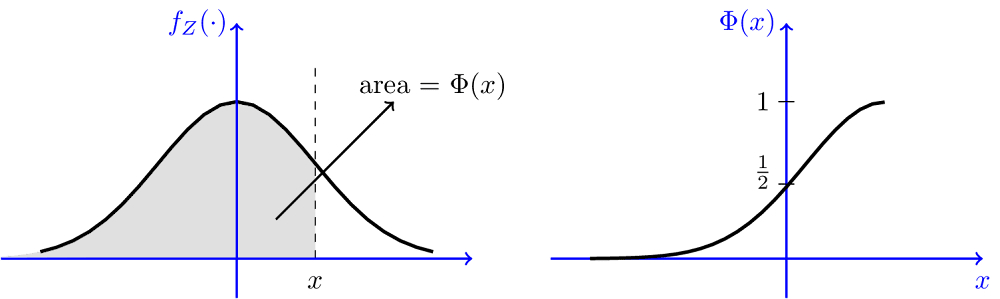
\includegraphics[width=0.7\linewidth]{images/Phi_b} \caption{The $\Phi$ and $\phi$ ($f_Z(.)$) functions (CDF and pdf of standard normal).}\label{fig:fig1}
    \end{figure}
\end{itemize}

Alternatively, use \textbf{the HTML approach}, and enclose the caption inside \texttt{\textless{}figcaption\textgreater{}}.

\begin{itemize}
\tightlist
\item
  Benefit: You can type equations as you normally do. Don't need to escape backslashes as using the R code blocks in the example above.
\item
  {Drawback: You need to manually add figure numbering.}
\end{itemize}

❗️That means, when you change the order of sections or figures in your webpage, the numbering will be a mess. You need to change all capitals manually.

\begin{Shaded}
\begin{Highlighting}[]
\DataTypeTok{\textless{}}\KeywordTok{figure}\DataTypeTok{\textgreater{}} 
\DataTypeTok{\textless{}}\KeywordTok{img}\OtherTok{ src}\OperatorTok{=}\StringTok{"https://drive.google.com/thumbnail?id=1nxfdIKXgZvOqXVSeA3h\_hf0yxmsM361l}\ErrorTok{\&}\StringTok{sz=w1000"}\OtherTok{ alt}\OperatorTok{=}\StringTok{"Phi\_b"}\OtherTok{ style}\OperatorTok{=}\StringTok{"display: block; margin{-}right: auto; margin{-}left: auto; zoom:80\%;"}\OtherTok{ }\DataTypeTok{/\textgreater{}}
\DataTypeTok{\textless{}}\KeywordTok{figcaption}\DataTypeTok{\textgreater{}}\NormalTok{Fig.1 The $\textbackslash{}Phi$ and $\textbackslash{}phi$ ($f\_Z(.)$) functions (CDF and pdf of standard normal).}\DataTypeTok{\textless{}/}\KeywordTok{figcaption}\DataTypeTok{\textgreater{}}
\DataTypeTok{\textless{}/}\KeywordTok{figure}\DataTypeTok{\textgreater{}}
\end{Highlighting}
\end{Shaded}

Fig.1 The \(\Phi\) and \(\phi\) (\(f_Z(.)\)) functions (CDF and pdf of standard normal).

\begin{center}\rule{0.5\linewidth}{0.5pt}\end{center}

\subsection*{Refer to another figure in figure caption}\label{refer-to-another-figure-in-figure-caption}
\addcontentsline{toc}{subsection}{Refer to another figure in figure caption}

Just need to use double backslash \texttt{\textbackslash{}\textbackslash{}@ref(fig:xxx)} in the figure caption.

Use example:

We first generate the figure to be referenced.

\begin{Shaded}
\begin{Highlighting}[]
\InformationTok{\textasciigrave{}\textasciigrave{}\textasciigrave{}\{r firstplot, out.width="60\%", fig.cap="Source Figure to be referred to."\}}
\InformationTok{library(ggplot2)}
\InformationTok{p \textless{}{-} ggplot(mtcars, aes(wt, mpg))}
\InformationTok{plot\_A \textless{}{-} p + geom\_point()}
\InformationTok{plot\_A}
\InformationTok{\textasciigrave{}\textasciigrave{}\textasciigrave{}}
\end{Highlighting}
\end{Shaded}

\textbackslash begin\{figure\}
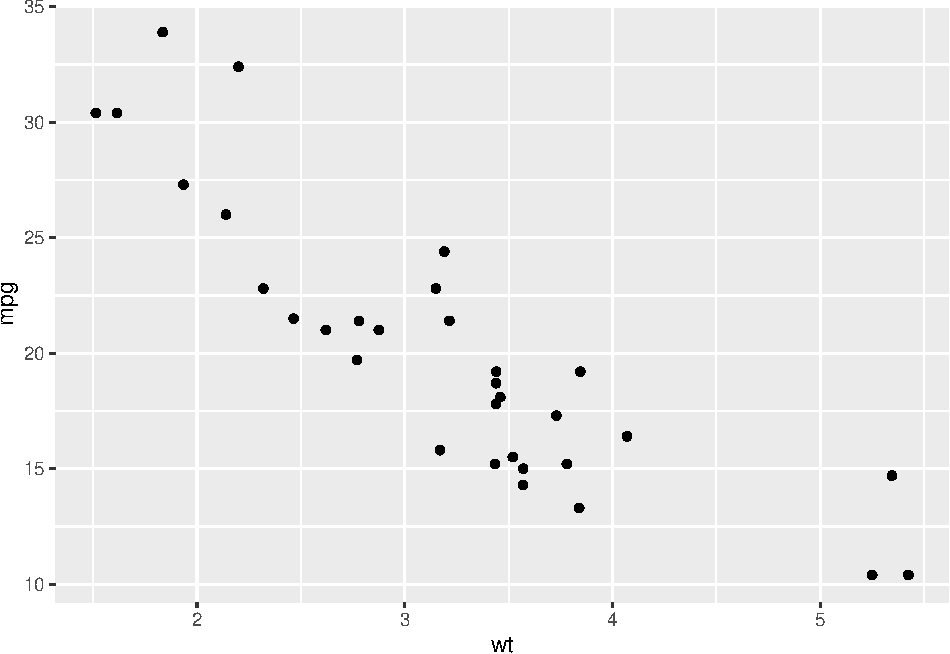
\includegraphics[width=0.6\linewidth]{0206-Rmd-Figure_files/figure-latex/firstplot-1} \textbackslash caption\{Source Figure to be referenced. \textbf{Note that when specifying \texttt{out.width="60\%"}, the text in the figure is scaled too small.}\}\label{fig:firstplot}
\textbackslash end\{figure\}

Now a second plot with a reference to Fig.: \ref{fig:firstplot}.

\begin{Shaded}
\begin{Highlighting}[]
\InformationTok{\textasciigrave{}\textasciigrave{}\textasciigrave{}\{r secondplot, fig.cap = "This is the same as Fig.: \textbackslash{}\textbackslash{}@ref(fig:firstplot) but now with a red line." \}}
\InformationTok{plot\_A + geom\_line(alpha = .75,col = "red")}
\InformationTok{\textasciigrave{}\textasciigrave{}\textasciigrave{}}
\end{Highlighting}
\end{Shaded}

\begin{figure}
\centering
\pandocbounded{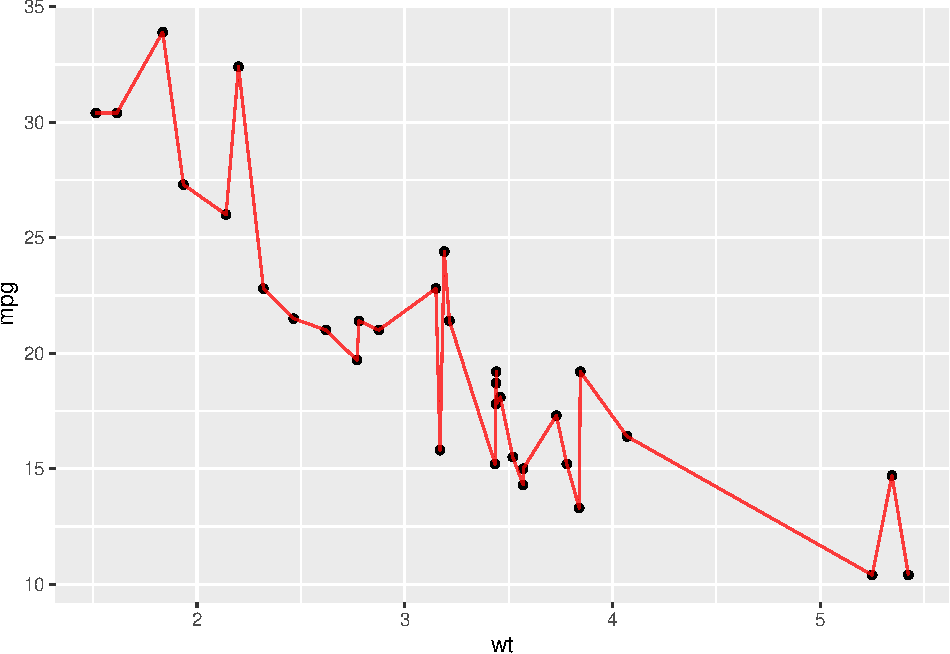
\includegraphics[keepaspectratio]{0206-Rmd-Figure_files/figure-latex/secondplot-1.pdf}}
\caption{\label{fig:secondplot}This is the same as Fig.: \ref{fig:firstplot} but now with a red line and \texttt{out.width="100\%"}.}
\end{figure}

\section{Tables}\label{tables}

{\textbf{Cross reference tables}}

Using \texttt{bookdown} cmd: \texttt{\textbackslash{}@ref(tab:chunk-label)}.

Note that you must provide \texttt{caption} option in \texttt{kable()}. Otherwise the table won't be numbered.

\begin{Shaded}
\begin{Highlighting}[]
\NormalTok{And see Table \textbackslash{}@ref(tab:mtcars).}

\InformationTok{\textasciigrave{}\textasciigrave{}\textasciigrave{}\{r mtcars, echo=FALSE\}}
\InformationTok{knitr::kable(mtcars[1:5, 1:5], caption = "The mtcars data.")}
\InformationTok{\textasciigrave{}\textasciigrave{}\textasciigrave{}}
\end{Highlighting}
\end{Shaded}

Refer to the Table \ref{tab:mtcars}.

\begin{table}

\caption{\label{tab:mtcars}The mtcars data.}
\centering
\begin{tabular}[t]{l|r|r|r|r|r}
\hline
  & mpg & cyl & disp & hp & drat\\
\hline
Mazda RX4 & 21.0 & 6 & 160 & 110 & 3.90\\
\hline
Mazda RX4 Wag & 21.0 & 6 & 160 & 110 & 3.90\\
\hline
Datsun 710 & 22.8 & 4 & 108 & 93 & 3.85\\
\hline
Hornet 4 Drive & 21.4 & 6 & 258 & 110 & 3.08\\
\hline
Hornet Sportabout & 18.7 & 8 & 360 & 175 & 3.15\\
\hline
\end{tabular}
\end{table}

The following is useful when you want to copy-and-paste R output from console to other document, e.g., markdown.

\begin{Shaded}
\begin{Highlighting}[]
\NormalTok{knitr}\SpecialCharTok{::}\FunctionTok{kable}\NormalTok{(mtcars[}\DecValTok{1}\SpecialCharTok{:}\DecValTok{5}\NormalTok{, }\DecValTok{1}\SpecialCharTok{:}\DecValTok{5}\NormalTok{], }\AttributeTok{format=}\StringTok{"pipe"}\NormalTok{)}
\SpecialCharTok{|}                  \ErrorTok{|}\NormalTok{  mpg}\SpecialCharTok{|}\NormalTok{ cyl}\SpecialCharTok{|}\NormalTok{ disp}\SpecialCharTok{|}\NormalTok{  hp}\SpecialCharTok{|}\NormalTok{ drat}\SpecialCharTok{|}
\ErrorTok{|:}\SpecialCharTok{{-}{-}{-}{-}{-}{-}{-}{-}{-}{-}{-}{-}{-}{-}{-}{-}{-}}\ErrorTok{|}\SpecialCharTok{{-}{-}{-}{-}}\ErrorTok{:|}\SpecialCharTok{{-}{-}{-}}\ErrorTok{:|}\SpecialCharTok{{-}{-}{-}{-}}\ErrorTok{:|}\SpecialCharTok{{-}{-}{-}}\ErrorTok{:|}\SpecialCharTok{{-}{-}{-}{-}}\ErrorTok{:|}
\ErrorTok{|}\NormalTok{Mazda RX4         }\SpecialCharTok{|} \FloatTok{21.0}\SpecialCharTok{|}   \DecValTok{6}\SpecialCharTok{|}  \DecValTok{160}\SpecialCharTok{|} \DecValTok{110}\SpecialCharTok{|} \FloatTok{3.90}\SpecialCharTok{|}
\ErrorTok{|}\NormalTok{Mazda RX4 Wag     }\SpecialCharTok{|} \FloatTok{21.0}\SpecialCharTok{|}   \DecValTok{6}\SpecialCharTok{|}  \DecValTok{160}\SpecialCharTok{|} \DecValTok{110}\SpecialCharTok{|} \FloatTok{3.90}\SpecialCharTok{|}
\ErrorTok{|}\NormalTok{Datsun }\DecValTok{710}        \SpecialCharTok{|} \FloatTok{22.8}\SpecialCharTok{|}   \DecValTok{4}\SpecialCharTok{|}  \DecValTok{108}\SpecialCharTok{|}  \DecValTok{93}\SpecialCharTok{|} \FloatTok{3.85}\SpecialCharTok{|}
\ErrorTok{|}\NormalTok{Hornet }\DecValTok{4}\NormalTok{ Drive    }\SpecialCharTok{|} \FloatTok{21.4}\SpecialCharTok{|}   \DecValTok{6}\SpecialCharTok{|}  \DecValTok{258}\SpecialCharTok{|} \DecValTok{110}\SpecialCharTok{|} \FloatTok{3.08}\SpecialCharTok{|}
\ErrorTok{|}\NormalTok{Hornet Sportabout }\SpecialCharTok{|} \FloatTok{18.7}\SpecialCharTok{|}   \DecValTok{8}\SpecialCharTok{|}  \DecValTok{360}\SpecialCharTok{|} \DecValTok{175}\SpecialCharTok{|} \FloatTok{3.15}\SpecialCharTok{|}
\end{Highlighting}
\end{Shaded}

\begin{center}\rule{0.5\linewidth}{0.5pt}\end{center}

\subsection{\texorpdfstring{\texttt{knitr::kable}}{knitr::kable}}\label{knitrkable}

\texttt{knitr::kable(x,\ digits,\ caption=NULL,\ escape=TRUE)} Create tables in LaTeX, HTML, Markdown and reStructuredText.

\begin{itemize}
\item
  \texttt{caption} The table caption. In order to number the table, mut specify the \texttt{caption} argument.
\item
  \texttt{format} Possible values are \texttt{latex}, \texttt{html}, \texttt{pipe} (Pandoc's pipe tables), \texttt{simple} (Pandoc's simple tables), \texttt{rst}, and \texttt{jira}.

  The value of this argument will be {automatically determined} if the function is called within a \textbf{knitr} document.
\item
  \texttt{digits} Maximum number of digits for numeric columns, passed to \texttt{round()}.
\item
  \texttt{col.names} Rename columns.
\item
  \texttt{escape=TRUE} Whether to escape special characters when producing HTML or LaTeX tables. Default is \texttt{TRUE}, special characters will either be escaped or substituted. For example, \texttt{\$} is escaped as \texttt{\textbackslash{}\$}, \texttt{\_} is escaped as \texttt{\textbackslash{}\_}, and \texttt{\textbackslash{}} is substituted with \texttt{\textbackslash{}textbackslash\{\}}

  \begin{itemize}
  \tightlist
  \item
    When set to \texttt{FALSE}, you have to make sure \textbf{yourself} that special characters will not trigger syntax errors in LaTeX or HTML.
  \item
    Common special LaTeX characters include \texttt{\#}, \texttt{\%}, \texttt{\&}, \texttt{\{}, and \texttt{\}}. Common special HTML characters include \texttt{\&}, \texttt{\textless{}}, \texttt{\textgreater{}}, and \texttt{"}. You need to be cautious when generating tables with \texttt{escape\ =\ FALSE}, and make sure you are using the special characters in the right way. It is a very common mistake to use \texttt{escape\ =\ FALSE} and include \texttt{\%} or \texttt{\_} in column names or the caption of a LaTeX table without realizing that they are special.
  \end{itemize}
\item
  \texttt{align} Column alignment: a character \textbf{vector} consisting of \texttt{\textquotesingle{}l\textquotesingle{}} (left), \texttt{\textquotesingle{}c\textquotesingle{}} (center) and/or \texttt{\textquotesingle{}r\textquotesingle{}} (right).

  \begin{itemize}
  \tightlist
  \item
    By default or if \texttt{align\ =\ NULL}, {numeric columns are right-aligned}, and {other columns are left-aligned}.
  \item
    If only one character is provided, that will apply to all columns.
  \item
    If a vector is provided, will map to each individual column specifically.
  \end{itemize}
\item
  Missing values (\texttt{NA}) in the table are displayed as \texttt{NA} by default. If you want to display them with other characters, you can set the option \texttt{knitr.kable.NA}, e.g.~{\texttt{options(knitr.kable.NA\ =\ \textquotesingle{}\textquotesingle{})}} in the YAML to hide \texttt{NA} values.
\item
  {\texttt{booktabs\ =\ TRUE}} use the booktabs package

  \begin{itemize}
  \tightlist
  \item
    \texttt{linesep\ =\ ""} remove the extra space after every five rows in kable output (with \texttt{booktabs} option)
  \end{itemize}
\end{itemize}

\begin{Shaded}
\begin{Highlighting}[]
\CommentTok{\# For Markdown tables, use \textasciigrave{}pipe\textasciigrave{} format}
\SpecialCharTok{\textgreater{}}\NormalTok{ knitr}\SpecialCharTok{::}\FunctionTok{kable}\NormalTok{(}\FunctionTok{head}\NormalTok{(mtcars[, }\DecValTok{1}\SpecialCharTok{:}\DecValTok{4}\NormalTok{]), }\AttributeTok{format=}\StringTok{"pipe"}\NormalTok{)}
\SpecialCharTok{|}                  \ErrorTok{|}\NormalTok{  mpg}\SpecialCharTok{|}\NormalTok{ cyl}\SpecialCharTok{|}\NormalTok{ disp}\SpecialCharTok{|}\NormalTok{  hp}\SpecialCharTok{|}
\ErrorTok{|:}\SpecialCharTok{{-}{-}{-}{-}{-}{-}{-}{-}{-}{-}{-}{-}{-}{-}{-}{-}{-}}\ErrorTok{|}\SpecialCharTok{{-}{-}{-}{-}}\ErrorTok{:|}\SpecialCharTok{{-}{-}{-}}\ErrorTok{:|}\SpecialCharTok{{-}{-}{-}{-}}\ErrorTok{:|}\SpecialCharTok{{-}{-}{-}}\ErrorTok{:|}
\ErrorTok{|}\NormalTok{Mazda RX4         }\SpecialCharTok{|} \FloatTok{21.0}\SpecialCharTok{|}   \DecValTok{6}\SpecialCharTok{|}  \DecValTok{160}\SpecialCharTok{|} \DecValTok{110}\SpecialCharTok{|}
\ErrorTok{|}\NormalTok{Mazda RX4 Wag     }\SpecialCharTok{|} \FloatTok{21.0}\SpecialCharTok{|}   \DecValTok{6}\SpecialCharTok{|}  \DecValTok{160}\SpecialCharTok{|} \DecValTok{110}\SpecialCharTok{|}
\ErrorTok{|}\NormalTok{Datsun }\DecValTok{710}        \SpecialCharTok{|} \FloatTok{22.8}\SpecialCharTok{|}   \DecValTok{4}\SpecialCharTok{|}  \DecValTok{108}\SpecialCharTok{|}  \DecValTok{93}\SpecialCharTok{|}
\ErrorTok{|}\NormalTok{Hornet }\DecValTok{4}\NormalTok{ Drive    }\SpecialCharTok{|} \FloatTok{21.4}\SpecialCharTok{|}   \DecValTok{6}\SpecialCharTok{|}  \DecValTok{258}\SpecialCharTok{|} \DecValTok{110}\SpecialCharTok{|}
\ErrorTok{|}\NormalTok{Hornet Sportabout }\SpecialCharTok{|} \FloatTok{18.7}\SpecialCharTok{|}   \DecValTok{8}\SpecialCharTok{|}  \DecValTok{360}\SpecialCharTok{|} \DecValTok{175}\SpecialCharTok{|}
\ErrorTok{|}\NormalTok{Valiant           }\SpecialCharTok{|} \FloatTok{18.1}\SpecialCharTok{|}   \DecValTok{6}\SpecialCharTok{|}  \DecValTok{225}\SpecialCharTok{|} \DecValTok{105}\SpecialCharTok{|}

\CommentTok{\# For Plain tables in txt, \textasciigrave{}simple\textasciigrave{} is useful}
\ErrorTok{\textgreater{}}\NormalTok{ knitr}\SpecialCharTok{::}\FunctionTok{kable}\NormalTok{(}\FunctionTok{head}\NormalTok{(mtcars[, }\DecValTok{1}\SpecialCharTok{:}\DecValTok{4}\NormalTok{]), }\StringTok{"simple"}\NormalTok{) }
\NormalTok{                      mpg   cyl   disp    hp}
\SpecialCharTok{{-}{-}{-}{-}{-}{-}{-}{-}{-}{-}{-}{-}{-}{-}{-}{-}{-}{-}}  \SpecialCharTok{{-}{-}{-}{-}{-}}  \SpecialCharTok{{-}{-}{-}{-}}  \SpecialCharTok{{-}{-}{-}{-}{-}}  \SpecialCharTok{{-}{-}{-}{-}}
\NormalTok{Mazda RX4            }\FloatTok{21.0}     \DecValTok{6}    \DecValTok{160}   \DecValTok{110}
\NormalTok{Mazda RX4 Wag        }\FloatTok{21.0}     \DecValTok{6}    \DecValTok{160}   \DecValTok{110}
\NormalTok{Datsun }\DecValTok{710}           \FloatTok{22.8}     \DecValTok{4}    \DecValTok{108}    \DecValTok{93}
\NormalTok{Hornet }\DecValTok{4}\NormalTok{ Drive       }\FloatTok{21.4}     \DecValTok{6}    \DecValTok{258}   \DecValTok{110}
\NormalTok{Hornet Sportabout    }\FloatTok{18.7}     \DecValTok{8}    \DecValTok{360}   \DecValTok{175}
\NormalTok{Valiant              }\FloatTok{18.1}     \DecValTok{6}    \DecValTok{225}   \DecValTok{105}
\end{Highlighting}
\end{Shaded}

\begin{center}\rule{0.5\linewidth}{0.5pt}\end{center}

\subsection{Data frame printing}\label{data-frame-printing}

To show the \texttt{tibble} information (number of row/columns, and group information) along with paged output, we can write a custom function by modifying the \href{https://github.com/rstudio/rmarkdown/blob/main/R/html_paged.R\#L241-L248}{\texttt{print.paged\_df}} function (which is used internally by rmarkdown for the \texttt{df\_print} feature) and use CSS to nicely format the output.

\url{https://stackoverflow.com/a/76014674/10108921}

{\textbf{Paged df}}

\begin{itemize}
\tightlist
\item
  \url{https://bookdown.org/yihui/rmarkdown/html-document.html\#tab:paged}
\item
  \url{https://github.com/rstudio/rmarkdown/issues/1403}
\end{itemize}

\begin{Shaded}
\begin{Highlighting}[]
\CommentTok{{-}{-}{-}}
\AnnotationTok{title:}\CommentTok{ "Use caption with df\_print set to page"}
\AnnotationTok{date:}\CommentTok{ "2025{-}04{-}14"}
\AnnotationTok{output:}
\CommentTok{  bookdown::html\_document2:}
\CommentTok{    df\_print: paged}
\CommentTok{{-}{-}{-}}
\end{Highlighting}
\end{Shaded}

When the \texttt{df\_print} option is set to \texttt{paged}, tables are printed as HTML tables with support for pagination over rows and columns.

The possible values of the \texttt{df\_print} option for the \texttt{html\_document} format.

\begin{longtable}[]{@{}
  >{\raggedright\arraybackslash}p{(\linewidth - 2\tabcolsep) * \real{0.4118}}
  >{\raggedright\arraybackslash}p{(\linewidth - 2\tabcolsep) * \real{0.5882}}@{}}
\toprule\noalign{}
\begin{minipage}[b]{\linewidth}\raggedright
Option
\end{minipage} & \begin{minipage}[b]{\linewidth}\raggedright
Description
\end{minipage} \\
\midrule\noalign{}
\endhead
\bottomrule\noalign{}
\endlastfoot
\texttt{default} & Call the \texttt{print.data.frame} generic method; console output prefixed by \texttt{\#\#}; \\
\texttt{kable} & Use the \texttt{knitr::kable} function; looks nice but with no navigation for rows and columns, neither column types. \\
\texttt{tibble} & Use the \texttt{tibble::print.tbl\_df} function, this provides groups and counts of rows and columns info as if printing a \texttt{tibble}. \\
{\texttt{paged}} & Use \texttt{rmarkdown::paged\_table} to create a pageable table; \texttt{paged} looks best but slows down compilation significantly; \\
A custom function & Use the function to create the table \\
\end{longtable}

The possible values of the \texttt{df\_print} option for the \texttt{pdf\_document} format: \texttt{default}, \texttt{kable}, \texttt{tibble}, \texttt{paged}, or a custom function.

\begin{Shaded}
\begin{Highlighting}[]
\NormalTok{paged print}

\InformationTok{\textasciigrave{}\textasciigrave{}\textasciigrave{}\{r echo=TRUE, paged.print=TRUE\}}
\InformationTok{ggplot2::diamonds}
\InformationTok{\textasciigrave{}\textasciigrave{}\textasciigrave{}}

\NormalTok{default output}

\InformationTok{\textasciigrave{}\textasciigrave{}\textasciigrave{}\{r echo=TRUE, paged.print=FALSE\}}
\InformationTok{ggplot2::diamonds}
\InformationTok{\textasciigrave{}\textasciigrave{}\textasciigrave{}}

\NormalTok{kable output}

\InformationTok{\textasciigrave{}\textasciigrave{}\textasciigrave{}\{r echo=TRUE\}}
\InformationTok{knitr::kable(ggplot2::diamonds[1:10, ])}
\InformationTok{\textasciigrave{}\textasciigrave{}\textasciigrave{}}
\end{Highlighting}
\end{Shaded}

\texttt{kable} output doesn't provide tibble informations.

Available options for \texttt{paged} tables:

\begin{longtable}[]{@{}
  >{\raggedright\arraybackslash}p{(\linewidth - 2\tabcolsep) * \real{0.2090}}
  >{\raggedright\arraybackslash}p{(\linewidth - 2\tabcolsep) * \real{0.7910}}@{}}
\toprule\noalign{}
\begin{minipage}[b]{\linewidth}\raggedright
Option
\end{minipage} & \begin{minipage}[b]{\linewidth}\raggedright
Description
\end{minipage} \\
\midrule\noalign{}
\endhead
\bottomrule\noalign{}
\endlastfoot
max.print & The number of rows to print. \\
rows.print & The number of rows to display. \\
cols.print & The number of columns to display. \\
cols.min.print & The minimum number of columns to display. \\
pages.print & The number of pages to display under page navigation. \\
paged.print & When set to \texttt{FALSE} turns off paged tables. \\
rownames.print & When set to \texttt{FALSE} turns off row names. \\
\end{longtable}

These options are specified in each chunk like below:

\begin{Shaded}
\begin{Highlighting}[]
\InformationTok{\textasciigrave{}\textasciigrave{}\textasciigrave{}\{r cols.print=3, rows.print=3\}}
\InformationTok{mtcars}
\InformationTok{\textasciigrave{}\textasciigrave{}\textasciigrave{}}
\end{Highlighting}
\end{Shaded}

For \textbf{pdf\_document}, it is possible to write LaTex code directly.

\begin{Shaded}
\begin{Highlighting}[]
\InformationTok{\textasciigrave{}\textasciigrave{}\textasciigrave{}\{=latex\}}
\InformationTok{\textbackslash{}begin\{tabular\}\{ll\}}
\InformationTok{A \& B \textbackslash{}\textbackslash{}}
\InformationTok{A \& B \textbackslash{}\textbackslash{}}
\InformationTok{\textbackslash{}end\{tabular\}}
\InformationTok{\textasciigrave{}\textasciigrave{}\textasciigrave{}}
\end{Highlighting}
\end{Shaded}

Do not forget the equal sign before \texttt{latex}, i.e., it is \texttt{=latex} instead of \texttt{latex}.

\begin{center}\rule{0.5\linewidth}{0.5pt}\end{center}

\subsection{Stargazer}\label{stargazer}

\texttt{stargazer} print nice \textbf{tables} in \texttt{Rmd}.

\url{https://libguides.princeton.edu/c.php?g=1326286&p=9763596\#s-lg-box-wrapper-36305037}

\begin{itemize}
\item
  Passing a data frame to stargazer package creates a {summary statistic table}.
\item
  Passing a regression object creates a nice {regression table}.\\
\item
  \texttt{stargaer} does not work with \texttt{anova} table, use \texttt{pander::pander} instead.
\end{itemize}

Text table

\begin{Shaded}
\begin{Highlighting}[]
\InformationTok{\textasciigrave{}\textasciigrave{}\textasciigrave{}\{r descrptive{-}analysis{-}text, comment = \textquotesingle{}\textquotesingle{}\}}
\InformationTok{apply(data[,{-}1], 2, get\_stat) \%\textgreater{}\% }
\InformationTok{    stargazer(type = "text", digits=2)}
\InformationTok{\textasciigrave{}\textasciigrave{}\textasciigrave{}}
\end{Highlighting}
\end{Shaded}

HTML table, note that need to specify \texttt{results="asis"}.

\begin{itemize}
\tightlist
\item
  \texttt{*}'s do not show properly, need to specify as footnote manually.
\end{itemize}

\begin{Shaded}
\begin{Highlighting}[]
\InformationTok{\textasciigrave{}\textasciigrave{}\textasciigrave{}\{r descrptive{-}analysis{-}html, results="asis"\}}
\InformationTok{apply(data[,{-}1], 2, get\_stat) \%\textgreater{}\% }
\InformationTok{    stargazer(type = "html", digits=2, }
\InformationTok{              notes = "\textless{}span\textgreater{}\&\#42;\textless{}/span\textgreater{}: p\textless{}0.1; \textless{}span\textgreater{}\&\#42;\&\#42;\textless{}/span\textgreater{}: \textless{}strong\textgreater{}p\textless{}0.05\textless{}/strong\textgreater{}; \textless{}span\textgreater{}\&\#42;\&\#42;\&\#42;\textless{}/span\textgreater{}: p\textless{}0.01 \textless{}br\textgreater{} Standard errors in the parentheses.",}
\InformationTok{              notes.append = F)}
\InformationTok{\textasciigrave{}\textasciigrave{}\textasciigrave{}}
\end{Highlighting}
\end{Shaded}

\begin{itemize}
\tightlist
\item
  \texttt{type} specify output table format. Possible values: \texttt{latex} (default for latex code), \texttt{html}, and \texttt{text}. Need to specify to \texttt{html} in html outputs.
\item
  \texttt{digits} an integer that indicates how many decimal places should be used. A value of \texttt{NULL} indicates that no rounding should be done at all, and that all available decimal places should be reported. Defaults to 3 digits.
\item
  \texttt{notes} a character vector containing notes to be included below the table.
\item
  \texttt{notes.append=FALSE} a logical value that indicates whether \texttt{notes} should be appended to the standard note(s) associated with the table's \texttt{style} (typically an explanation of significance cutoffs).

  \begin{itemize}
  \tightlist
  \item
    Defaults to \texttt{TRUE}.
  \item
    If the argument's value is set to \texttt{FALSE}, the character strings provided in \texttt{notes} will replace any existing/default notes.
  \end{itemize}
\end{itemize}

Add a blank line under the \texttt{stargazer} table: \texttt{\&nbsp;} with a blank line above and below.

\textbf{Cross reference \texttt{stargazer} tables.}

\begin{itemize}
\item
  {In pdf output}, use \texttt{Table\ \textbackslash{}@ref(tab:reg-table)} or \texttt{Table\ \textbackslash{}ref\{tab:reg-table\}}.

\begin{Shaded}
\begin{Highlighting}[]
\NormalTok{Table \textbackslash{}@ref(tab:reg{-}table) summarize the regression results in a table.}

\InformationTok{\textasciigrave{}\textasciigrave{}\textasciigrave{}\{r, include=TRUE, results=\textquotesingle{}asis\textquotesingle{}\}}
\InformationTok{stargazer(capm\_ml, FF\_ml, type=\textquotesingle{}latex\textquotesingle{}, header=FALSE,}
\InformationTok{          digits=4, no.space = TRUE,}
\InformationTok{          title="Regression Results for META",}
\InformationTok{          label = "tab:reg{-}table")}
\InformationTok{\textasciigrave{}\textasciigrave{}\textasciigrave{}}
\end{Highlighting}
\end{Shaded}

  \begin{itemize}
  \item
    {\texttt{header=FALSE}} is to suppress the \texttt{\%\ Table\ created\ by\ stargazer} header. This applies to only \texttt{latex} tables.
  \item
    \texttt{label="tab:reg-table"} is to specify the cross reference label for the table.
  \item
    {\texttt{table.placement\ =\ "H"}} set float to \texttt{H} to fix positions. Places the float at \emph{precisely} the location in the code. This requires the {\texttt{float}} LaTeX package. Remember to load it in the YAML.

    \begin{itemize}
    \item
      Defaults to \texttt{"!htbp"}.

      The \texttt{htbp} controls where the table or figure is placed. Tables and figures do not need to go where you put them in the text. LATEX moves them around to prevent large areas of white space from appearing in your paper.
      \texttt{h} (Here): Place the float here, i.e., \emph{approximately} at the same point it occurs in the source text (however, \emph{not exactly} at the spot)
      \texttt{t} (Top): Place the table at the top of the \emph{current} page
      \texttt{b} (Bottom): Place the table at the \emph{bottom} of the current page.
      \texttt{p} (Page): Place the table at the top of the \emph{next} page.
      \texttt{!}: Override internal parameters LaTeX uses for determining ``good'' float positions.
    \end{itemize}
  \item
    \texttt{notes.align} \texttt{"l"} for left alignment, \texttt{"r"} for right alignment, and \texttt{"c"} for centering. This argument is not case-sensitive.
  \item
    \texttt{single.row\ =\ TRUE} to put coefficients and standard errors on same line
  \item
    {\texttt{no.space\ =\ TRUE}} to remove the spaces after each line of coefficients
  \item
    \texttt{font.size\ =\ "small"} to make font size smaller
  \item
    \texttt{column.labels} a character vector of labels for columns in regression tables.
  \item
    \texttt{column.separate} a numeric vector that specifies how \texttt{column.labels} should be laid out across regression table columns. A value of \texttt{c(2,\ 1,\ 3)}, for instance, will apply the first label to the two first columns, the second label to the third column, and the third label will apply to the following three columns (i.e., columns number four, five and six).
  \item
    \texttt{dep.var.labels} and \texttt{covariate.labels} labels for dependant variables
  \item
    {\texttt{covariate.labels}} labels for covariates in the regression tables.

    Can provide latex symbols in the labels, need to escape special symbols though.

\begin{Shaded}
\begin{Highlighting}[]
\FunctionTok{stargazer}\NormalTok{(mod\_sel\_lm\_mtcars, }
      \AttributeTok{covariate.labels =} 
        \FunctionTok{c}\NormalTok{(}\StringTok{"(Intercept)"}\NormalTok{, }\StringTok{"drat"}\NormalTok{, }\StringTok{"hp"}\NormalTok{, }\StringTok{"$w\_\{i\}$"}\NormalTok{,}
          \StringTok{"}\SpecialCharTok{\textbackslash{}\textbackslash{}}\StringTok{textit\{k\}"}\NormalTok{, }\StringTok{"logLik"}\NormalTok{, }\StringTok{"AICc"}\NormalTok{, }\StringTok{"}\SpecialCharTok{\textbackslash{}\textbackslash{}}\StringTok{Delta AICc"}\NormalTok{))}
\end{Highlighting}
\end{Shaded}
  \item
    \texttt{align=FALSE} a logical value indicating whether numeric values in the same column should be aligned at the decimal mark in LaTeX output.
  \item
    \texttt{add.lines} add a row(s), such as reporting fixed effects.

\begin{Shaded}
\begin{Highlighting}[]
\FunctionTok{stargazer}\NormalTok{(output, output2, }\AttributeTok{type =} \StringTok{"html"}\NormalTok{,}
          \AttributeTok{add.lines =} \FunctionTok{list}\NormalTok{(}\FunctionTok{c}\NormalTok{(}\StringTok{"Fixed effects?"}\NormalTok{, }\StringTok{"No"}\NormalTok{, }\StringTok{"No"}\NormalTok{),}
                           \FunctionTok{c}\NormalTok{(}\StringTok{"Results believable?"}\NormalTok{, }\StringTok{"Maybe"}\NormalTok{, }\StringTok{"Try again later"}\NormalTok{)))}
\end{Highlighting}
\end{Shaded}
  \end{itemize}
\item
  {In html output}, cross references to stargazer tables are not so straightforward.

  \texttt{label} option in \texttt{stargazer} does not work. Cannot use chunk labels either.

\begin{Shaded}
\begin{Highlighting}[]
\InformationTok{\textasciigrave{}\textasciigrave{}\textasciigrave{}\{r fit{-}age, echo=FALSE, results=\textquotesingle{}asis\textquotesingle{}, fig.cap="Logistic regression of CHD on age."\}}
\InformationTok{\# Use title caption from fig.cap}
\InformationTok{tit \textless{}{-} knitr::opts\_current$get("fig.cap")}
\InformationTok{\# Adding caption for html output}
\InformationTok{tit\_html \textless{}{-} paste0(\textquotesingle{}\textless{}span id="tab:\textquotesingle{},}
\InformationTok{                   knitr::opts\_current$get("label"),}
\InformationTok{                   \textquotesingle{}"\textgreater{}(\#tab:\textquotesingle{},}
\InformationTok{                   knitr::opts\_current$get("label"),}
\InformationTok{                   \textquotesingle{})\textless{}/span\textgreater{}\textquotesingle{},}
\InformationTok{                   tit)}
\InformationTok{stargazer::stargazer(fit.age,}
\InformationTok{          label = paste0("tab:", knitr::opts\_current$get("label")),}
\InformationTok{          title = ifelse(knitr::is\_latex\_output(), tit, tit\_html),}
\InformationTok{          type = ifelse(knitr::is\_latex\_output(),"latex","html"),}
\InformationTok{          notes = "\textless{}span\textgreater{}\&\#42;\textless{}/span\textgreater{}: p\textless{}0.1; \textless{}span\textgreater{}\&\#42;\&\#42;\textless{}/span\textgreater{}: \textless{}strong\textgreater{}p\textless{}0.05\textless{}/strong\textgreater{}; \textless{}span\textgreater{}\&\#42;\&\#42;\&\#42;\textless{}/span\textgreater{}: p\textless{}0.01 \textless{}br\textgreater{} Standard errors in the parentheses.",}
\InformationTok{          notes.append = F,}
\InformationTok{          header = F}
\InformationTok{          )}
\InformationTok{\textasciigrave{}\textasciigrave{}\textasciigrave{}}

\NormalTok{Here is another reference to stargazer Table \textbackslash{}@ref(tab:fit{-}age).}
\end{Highlighting}
\end{Shaded}

  Don't change things unless it is absolutely necessary. Run the code chunk before compiling the whole website. It gets slowly as the website gets larger.

  \texttt{stargazer::stargazer()} the \texttt{::} is necessary, and \texttt{header=F} is necessary and should be place at the end, otherwise will have errors as follows.

\begin{Shaded}
\begin{Highlighting}[]
\NormalTok{Error }\ControlFlowTok{in} \StringTok{\textasciigrave{}}\AttributeTok{.stargazer.wrap()}\StringTok{\textasciigrave{}}\SpecialCharTok{:}
\SpecialCharTok{!}\NormalTok{ argument is missing, with no default}
\NormalTok{Backtrace}\SpecialCharTok{:}
 \FloatTok{1.}\NormalTok{ stargazer}\SpecialCharTok{::}\FunctionTok{stargazer}\NormalTok{(...)}
 \FloatTok{2.}\NormalTok{ stargazer}\SpecialCharTok{:::}\FunctionTok{.stargazer.wrap}\NormalTok{(...)}
\NormalTok{Execution halted}

\NormalTok{Exited with status }\FloatTok{1.}
\end{Highlighting}
\end{Shaded}

  Another example if you don't need to add footnotes.

\begin{Shaded}
\begin{Highlighting}[]
\InformationTok{\textasciigrave{}\textasciigrave{}\textasciigrave{}\{r mytable, results=\textquotesingle{}asis\textquotesingle{}, fig.cap="This is my table."\}}

\InformationTok{\# Use title caption from fig.cap}
\InformationTok{tit \textless{}{-} knitr::opts\_current$get("fig.cap")}

\InformationTok{\# Adding caption for html output}
\InformationTok{tit\_html \textless{}{-} paste0(\textquotesingle{}\textless{}span id="tab:\textquotesingle{},}
\InformationTok{                   knitr::opts\_current$get("label"),}
\InformationTok{                   \textquotesingle{}"\textgreater{}(\#tab:\textquotesingle{},}
\InformationTok{                   knitr::opts\_current$get("label"),}
\InformationTok{                   \textquotesingle{})\textless{}/span\textgreater{}\textquotesingle{},}
\InformationTok{                   tit)}

\InformationTok{stargazer::stargazer(fit.age,}
\InformationTok{                     label = paste0("tab:", knitr::opts\_current$get("label")),}
\InformationTok{                     title = ifelse(knitr::is\_latex\_output(), tit, tit\_html),}
\InformationTok{                     type = ifelse(knitr::is\_latex\_output(),"latex","html"),}
\InformationTok{                     header = F}
\InformationTok{                     )}
\InformationTok{\textasciigrave{}\textasciigrave{}\textasciigrave{}}

\NormalTok{Here is a reference to stargazer Table \textbackslash{}@ref(tab:mytable).}
\end{Highlighting}
\end{Shaded}
\end{itemize}

\textbf{Alignment of Stargazer Tables}

\begin{itemize}
\item
  In PDF, the tables will be in the center by default.
\item
  However, when working with HTML output, you need to add CSS styling to adjust the table.
\end{itemize}

\begin{center}\rule{0.5\linewidth}{0.5pt}\end{center}

\subsection{\texorpdfstring{\texttt{kableExtra}}{kableExtra}}\label{kableextra}

The \textbf{kableExtra} package is designed to extend the basic functionality of tables produced using \texttt{knitr::kable()}.

\texttt{kableExtra::kable\_styling(bootstrap\_options\ =\ c("striped",\ "hover"),\ full\_width\ =\ FALSE)}

\begin{itemize}
\item
  \texttt{bootstrap\_options} A character vector for bootstrap table options. Please see package vignette or visit the w3schools' \href{https://www.w3schools.com/bootstrap/bootstrap_tables.asp}{Bootstrap Page} for more information. Possible options include \texttt{basic}, \texttt{striped}, \texttt{bordered}, \texttt{hover}, \texttt{condensed}, \texttt{responsive} and \texttt{none}.

  \begin{itemize}
  \tightlist
  \item
    \texttt{striped} alternating row colors
  \item
    \texttt{hover} Use the \texttt{:hover} selector on \texttt{tr} (table row) to {highlight table rows} on mouse over.
  \end{itemize}
\item
  \texttt{full\_width} A \texttt{TRUE} or \texttt{FALSE} variable controlling whether the HTML table should have 100\% the preferable format for \texttt{full\_width}. If not specified,

  \begin{itemize}
  \tightlist
  \item
    \texttt{TRUE} for a HTML table , will have full width by default but
  \item
    this option will be set to \texttt{FALSE} for a LaTeX table.
  \end{itemize}
\item
  \texttt{latex\_options} A character vector for \textbf{LaTeX} table options, i.e., won't have effecs on html tables.

  Possible options:

  \begin{longtable}[]{@{}
    >{\raggedright\arraybackslash}p{(\linewidth - 2\tabcolsep) * \real{0.2000}}
    >{\raggedright\arraybackslash}p{(\linewidth - 2\tabcolsep) * \real{0.8000}}@{}}
  \toprule\noalign{}
  \begin{minipage}[b]{\linewidth}\raggedright
  Arguments
  \end{minipage} & \begin{minipage}[b]{\linewidth}\raggedright
  Meanings
  \end{minipage} \\
  \midrule\noalign{}
  \endhead
  \bottomrule\noalign{}
  \endlastfoot
  \texttt{striped} & Add alternative row colors to the table. It will imports \texttt{LaTeX} package \texttt{xcolor} if enabled. \\
  \texttt{scale\_down} & useful for super \textbf{wide} table. It will automatically adjust the table to {fit the page width}. \\
  \texttt{repeat\_header} & only meaningful in a \textbf{long} table environment. It will let the header row repeat on every page in that long table. \\
  \texttt{hold\_position} & ``hold'' the floating table to the exact position. It is useful when the \texttt{LaTeX} table is contained in a \texttt{table} environment after you specified captions in \texttt{kable()}. It will force the table to stay in the position where it was created in the document. \\
  \texttt{HOLD\_position} & A stronger version of \texttt{hold\_position}. Requires the float package and specifies ⁠{[}H{]}⁠. \\
  \end{longtable}
\end{itemize}

Rows and columns can be grouped via the functions \texttt{pack\_rows()} and \texttt{add\_header\_above()}, respectively.

\texttt{scroll\_box(width\ =\ "100\%",\ height\ =\ "500px")} let you create a fixed height table while \textbf{making it scrollable}. This function only works for html long tables.

\begin{Shaded}
\begin{Highlighting}[]
\CommentTok{\# commonly used settings }
\NormalTok{table }\SpecialCharTok{\%\textgreater{}\%} 
\NormalTok{    knitr}\SpecialCharTok{::}\FunctionTok{kable}\NormalTok{(}\AttributeTok{digits =} \DecValTok{5}\NormalTok{) }\SpecialCharTok{\%\textgreater{}\%}
    \FunctionTok{kable\_styling}\NormalTok{(}\AttributeTok{bootstrap\_options =} \FunctionTok{c}\NormalTok{(}\StringTok{"striped"}\NormalTok{, }\StringTok{"hover"}\NormalTok{), }\AttributeTok{full\_width =} \ConstantTok{FALSE}\NormalTok{, }\AttributeTok{latex\_options=}\StringTok{"scale\_down"}\NormalTok{) }\SpecialCharTok{\%\textgreater{}\%} 
    \FunctionTok{scroll\_box}\NormalTok{(}\AttributeTok{width =} \StringTok{"100\%"}\NormalTok{, }\AttributeTok{height =} \StringTok{"500px"}\NormalTok{)}
\end{Highlighting}
\end{Shaded}

\begin{Shaded}
\begin{Highlighting}[]
\CommentTok{\# escape=TRUE, this makes your life easier, will output the table exactly as it is}
\NormalTok{result }\OtherTok{\textless{}{-}} \FunctionTok{read\_csv}\NormalTok{(}\StringTok{"\textasciitilde{}/Documents/GDP/data/reg\_result/IFE\_result.csv"}\NormalTok{)}
\NormalTok{result }\SpecialCharTok{\%\textgreater{}\%}
\NormalTok{  knitr}\SpecialCharTok{::}\FunctionTok{kable}\NormalTok{(}\AttributeTok{digits =} \DecValTok{5}\NormalTok{, }\AttributeTok{escape=}\NormalTok{T) }\SpecialCharTok{\%\textgreater{}\%}
  \FunctionTok{kable\_styling}\NormalTok{(}\AttributeTok{bootstrap\_options =} \FunctionTok{c}\NormalTok{(}\StringTok{"striped"}\NormalTok{, }\StringTok{"hover"}\NormalTok{), }\AttributeTok{full\_width =} \ConstantTok{FALSE}\NormalTok{, }\AttributeTok{latex\_options=}\StringTok{"scale\_down"}\NormalTok{)}
\end{Highlighting}
\end{Shaded}

\begin{Shaded}
\begin{Highlighting}[]
\CommentTok{\# escape=FALSE, have to specify escape by replace \textasciigrave{}*\textasciigrave{} to \textasciigrave{}\textbackslash{}\textbackslash{}\textbackslash{}\textbackslash{}*\textasciigrave{}}
\NormalTok{result }\OtherTok{\textless{}{-}} \FunctionTok{read\_csv}\NormalTok{(}\StringTok{"\textasciitilde{}/Documents/GDP/data/reg\_result/IFE\_result.csv"}\NormalTok{)}
\NormalTok{result }\OtherTok{\textless{}{-}}\NormalTok{ result }\SpecialCharTok{\%\textgreater{}\%} 
  \FunctionTok{mutate}\NormalTok{(}\AttributeTok{pval.symbol =} \FunctionTok{gsub}\NormalTok{(}\StringTok{"[*]"}\NormalTok{, }\StringTok{"}\SpecialCharTok{\textbackslash{}\textbackslash{}\textbackslash{}\textbackslash{}}\StringTok{*"}\NormalTok{, pval.symbol) )}
\NormalTok{result }\SpecialCharTok{\%\textgreater{}\%}
\NormalTok{  knitr}\SpecialCharTok{::}\FunctionTok{kable}\NormalTok{(}\AttributeTok{digits =} \DecValTok{5}\NormalTok{, }\AttributeTok{escape=}\ConstantTok{FALSE}\NormalTok{) }\SpecialCharTok{\%\textgreater{}\%}
  \FunctionTok{kable\_styling}\NormalTok{(}\AttributeTok{bootstrap\_options =} \FunctionTok{c}\NormalTok{(}\StringTok{"striped"}\NormalTok{, }\StringTok{"hover"}\NormalTok{), }\AttributeTok{full\_width =} \ConstantTok{FALSE}\NormalTok{, }\AttributeTok{latex\_options=}\StringTok{"scale\_down"}\NormalTok{)}
\end{Highlighting}
\end{Shaded}

\textbf{tables in pdf output}

\begin{Shaded}
\begin{Highlighting}[]
\NormalTok{reg\_data }\SpecialCharTok{\%\textgreater{}\%} 
    \FunctionTok{select}\NormalTok{(Date, adjusted, eRi, rmrf) }\SpecialCharTok{\%\textgreater{}\%}
    \FunctionTok{head}\NormalTok{(}\DecValTok{10}\NormalTok{) }\SpecialCharTok{\%\textgreater{}\%} 
\NormalTok{    knitr}\SpecialCharTok{::}\FunctionTok{kable}\NormalTok{(}\AttributeTok{digits =} \FunctionTok{c}\NormalTok{(}\DecValTok{0}\NormalTok{,}\DecValTok{2}\NormalTok{,}\DecValTok{4}\NormalTok{,}\DecValTok{4}\NormalTok{), }\AttributeTok{escape=}\NormalTok{T, }\AttributeTok{format =} \StringTok{"latex"}\NormalTok{, }\AttributeTok{booktabs =} \ConstantTok{TRUE}\NormalTok{, }\AttributeTok{linesep =} \StringTok{""}\NormalTok{ ) }\SpecialCharTok{\%\textgreater{}\%}
    \FunctionTok{kable\_styling}\NormalTok{(}\AttributeTok{latex\_options =} \FunctionTok{c}\NormalTok{(}\StringTok{"striped"}\NormalTok{), }\AttributeTok{full\_width =} \ConstantTok{FALSE}\NormalTok{, }\AttributeTok{stripe\_color =} \StringTok{"gray!15"}\NormalTok{)}
\end{Highlighting}
\end{Shaded}

\texttt{knitr::kable()} arguments

\begin{itemize}
\item
  \texttt{format\ =\ "latex"} specifies the output format.
\item
  \texttt{align\ =\ "l"} specifies column alignment.
\item
  \texttt{booktabs\ =\ TRUE} is generally recommended for formatting LaTeX tables.
\item
  \texttt{linesep\ =\ ""} prevents default behavior of extra space every five rows.
\end{itemize}

\texttt{kableExtra::kable\_styling()} arguments

\begin{itemize}
\tightlist
\item
  \texttt{position\ =\ "left"} places table on left hand side of page.
\item
  \texttt{latex\_options\ =\ c("striped",\ "repeat\_header")} implements table striping with repeated headers for tables that span multiple pages.
\item
  \texttt{stripe\_color\ =\ "gray!15"} species the stripe color using LaTeX color specification from the \href{https://mirror.mwt.me/ctan/macros/latex/contrib/xcolor/xcolor.pdf}{xcolor package} - this specifies a mix of 15\% gray and 85\% white.
\end{itemize}

\texttt{linebreak(x,\ align\ =\ "l",\ double\_escape\ =\ F,\ linebreaker\ =\ "\textbackslash{}n")} Make linebreak in LaTeX Table cells.

\begin{itemize}
\tightlist
\item
  \texttt{align="l"} Choose from ``l'', ``c'' or ``r''. Defaults to ``l''.
\end{itemize}

\textbf{Customize the looks for columns/rows}

\texttt{kableExtra::column\_spec(kable\_input)} this function allows users to select a column and then specify its look.

\texttt{row\_spec()} works similar with \texttt{column\_spec()} but defines specifications for rows.

\begin{itemize}
\tightlist
\item
  For the position of the target row, you don't need to count in header rows or the group labeling rows.
\item
  \texttt{row\_spec(row\ =\ 0,\ align=\textquotesingle{}c\textquotesingle{})} specify format of the header row. Here I want to center align headers.
\end{itemize}

\textbf{Add header rows to group columns}

\texttt{add\_header\_above()}. The header variable is supposed to be a named character with the names as new column names and values as column span. For your convenience, if column span equals to 1, you can ignore the \texttt{=1} part so the function below can be written as \texttt{add\_header\_above(c("",\ "Group\ 1"\ =\ 2,\ "Group\ 2"\ =\ 2,\ "Group\ 3"\ =\ 2))}.

\begin{Shaded}
\begin{Highlighting}[]
\FunctionTok{kbl}\NormalTok{(dt) }\SpecialCharTok{\%\textgreater{}\%}
  \FunctionTok{kable\_classic}\NormalTok{() }\SpecialCharTok{\%\textgreater{}\%}
  \FunctionTok{add\_header\_above}\NormalTok{(}\FunctionTok{c}\NormalTok{(}\StringTok{" "} \OtherTok{=} \DecValTok{1}\NormalTok{, }\StringTok{"Group 1"} \OtherTok{=} \DecValTok{2}\NormalTok{, }\StringTok{"Group 2"} \OtherTok{=} \DecValTok{2}\NormalTok{, }\StringTok{"Group 3"} \OtherTok{=} \DecValTok{2}\NormalTok{))}
\end{Highlighting}
\end{Shaded}

You can add another row of header on top.

\textbf{Group rows}

\texttt{collapse\_rows} will put repeating cells in columns into multi-row cells. The vertical alignment of the cell is controlled by \texttt{valign} with default as ``top''.

Not working for html output.

\begin{Shaded}
\begin{Highlighting}[]
\NormalTok{collapse\_rows\_dt }\OtherTok{\textless{}{-}} \FunctionTok{data.frame}\NormalTok{(}\AttributeTok{C1 =} \FunctionTok{c}\NormalTok{(}\FunctionTok{rep}\NormalTok{(}\StringTok{"a"}\NormalTok{, }\DecValTok{10}\NormalTok{), }\FunctionTok{rep}\NormalTok{(}\StringTok{"b"}\NormalTok{, }\DecValTok{5}\NormalTok{)),}
                 \AttributeTok{C2 =} \FunctionTok{c}\NormalTok{(}\FunctionTok{rep}\NormalTok{(}\StringTok{"c"}\NormalTok{, }\DecValTok{7}\NormalTok{), }\FunctionTok{rep}\NormalTok{(}\StringTok{"d"}\NormalTok{, }\DecValTok{3}\NormalTok{), }\FunctionTok{rep}\NormalTok{(}\StringTok{"c"}\NormalTok{, }\DecValTok{2}\NormalTok{), }\FunctionTok{rep}\NormalTok{(}\StringTok{"d"}\NormalTok{, }\DecValTok{3}\NormalTok{)),}
                 \AttributeTok{C3 =} \DecValTok{1}\SpecialCharTok{:}\DecValTok{15}\NormalTok{,}
                 \AttributeTok{C4 =} \FunctionTok{sample}\NormalTok{(}\FunctionTok{c}\NormalTok{(}\DecValTok{0}\NormalTok{,}\DecValTok{1}\NormalTok{), }\DecValTok{15}\NormalTok{, }\AttributeTok{replace =} \ConstantTok{TRUE}\NormalTok{))}
\FunctionTok{kbl}\NormalTok{(collapse\_rows\_dt, }\AttributeTok{align =} \StringTok{"c"}\NormalTok{) }\SpecialCharTok{\%\textgreater{}\%}
  \FunctionTok{kable\_paper}\NormalTok{(}\AttributeTok{full\_width =}\NormalTok{ F) }\SpecialCharTok{\%\textgreater{}\%}
  \FunctionTok{column\_spec}\NormalTok{(}\DecValTok{1}\NormalTok{, }\AttributeTok{bold =}\NormalTok{ T) }\SpecialCharTok{\%\textgreater{}\%}
  \FunctionTok{collapse\_rows}\NormalTok{(}\AttributeTok{columns =} \DecValTok{1}\SpecialCharTok{:}\DecValTok{2}\NormalTok{, }\AttributeTok{valign =} \StringTok{"top"}\NormalTok{)}
\end{Highlighting}
\end{Shaded}

Empty string as column name in \texttt{tibble}: use \texttt{setNames} or \texttt{attr}

\begin{Shaded}
\begin{Highlighting}[]
\NormalTok{df }\OtherTok{\textless{}{-}} \FunctionTok{tibble}\NormalTok{(}\StringTok{" "}\OtherTok{=}\DecValTok{1}\NormalTok{)}
\FunctionTok{setNames}\NormalTok{(df, }\StringTok{""}\NormalTok{)}
\CommentTok{\# \# A tibble: 1 x 1}
\CommentTok{\#      \textasciigrave{}\textasciigrave{}}
\CommentTok{\#   \textless{}dbl\textgreater{}}
\CommentTok{\# 1     1}

\FunctionTok{attr}\NormalTok{(df, }\StringTok{"names"}\NormalTok{) }\OtherTok{\textless{}{-}} \FunctionTok{c}\NormalTok{(}\StringTok{""}\NormalTok{)}
\end{Highlighting}
\end{Shaded}

\texttt{footnote()} add footnotes to tables. There are four notation systems in \texttt{footnote}, namely \texttt{general} (no prefix for footnotes), \texttt{number}, \texttt{alphabet} and \texttt{symbol}.

\textbf{Math in rmd tables}

\texttt{knitr::kable(x,\ escape=TRUE)}

\begin{itemize}
\tightlist
\item
  \texttt{escape=TRUE} whether to escape special characters when producing HTML or LaTeX tables.

  \begin{itemize}
  \tightlist
  \item
    Defaults to \texttt{TRUE}.
  \item
    When \texttt{escape\ =\ FALSE}, you have to make sure that special characters will not trigger syntax errors in LaTeX or HTML.
  \end{itemize}
\end{itemize}

You need to escape \texttt{\textbackslash{}} passed into R code.

\begin{Shaded}
\begin{Highlighting}[]
\InformationTok{\textasciigrave{}\textasciigrave{}\textasciigrave{}\{r, echo=FALSE\}}
\InformationTok{library(knitr)}

\InformationTok{mathy.df \textless{}{-} data.frame(site = c("A", "B"), }
\InformationTok{                       b0 = c(3, 4), }
\InformationTok{                       BA = c(1, 2))}

\InformationTok{colnames(mathy.df) \textless{}{-} c("Site", "$\textbackslash{}\textbackslash{}beta\_0$", "$\textbackslash{}\textbackslash{}beta\_A$")}

\InformationTok{kable(mathy.df, escape=FALSE)}
\InformationTok{\textasciigrave{}\textasciigrave{}\textasciigrave{}}
\end{Highlighting}
\end{Shaded}

It is possible to edit Latex table directly in \texttt{Rmd}.

\begin{itemize}
\tightlist
\item
  Don't enclose in \texttt{\$\$}.
\item
  Use \texttt{\textbackslash{}begin\{table\}} and start your table data.
\end{itemize}

\section{Rmd GitHub Pages}\label{rmd-github-pages}

\textbf{Stage-commit-push many files}

\begin{enumerate}
\def\labelenumi{\arabic{enumi}.}
\item
  Use the Terminal \texttt{git\ add\ .} to ``stage'' all the files that I want to commit as that's quicker than clicking on all the files often that I want to commit.
\item
  Go to RStudio \texttt{Commit\ Pending\ changes} icon (the white docs icon with a tick in a Git pane) to write the commit as I find \texttt{git\ commit\ -m\ "Write\ your\ message\ here"} a bit too long!
\item
  Use the Push and Pull buttons in RStudio as that's easier than typing \texttt{git\ push} or \texttt{git\ pull} in the terminal.
\end{enumerate}

\begin{center}\rule{0.5\linewidth}{0.5pt}\end{center}

\subsection*{Project structure}\label{project-structure}
\addcontentsline{toc}{subsection}{Project structure}

Note that the \textbf{minimum requirement for any R Markdown website} is that it have an \texttt{index.Rmd} file and a \texttt{\_site.yml} file.

If you execute the \texttt{rmarkdown::render\_site()} function from within the directory containing the website, the following will occur:

\begin{enumerate}
\def\labelenumi{\arabic{enumi}.}
\item
  All of the \texttt{*.Rmd} and \texttt{*.md} files in the root website directory will be rendered into HTML. Note, however, that Markdown files beginning with \texttt{\_} are not rendered (this is a convention to designate files that are to be included by top level Rmd documents as child documents).

  \begin{itemize}
  \tightlist
  \item
    \texttt{index.Rmd} controls the content on your main page.
  \end{itemize}
\item
  The generated HTML files and any supporting files (e.g., CSS and JavaScript) are copied into an output directory (\texttt{\_site} by default, on Github Pages the output folder is \texttt{docs}).

  The HTML files within the output directory are now ready to deploy as a standalone static website.
\end{enumerate}

\begin{center}\rule{0.5\linewidth}{0.5pt}\end{center}

\subsection*{\texorpdfstring{\texttt{\_site.yml} config}{\_site.yml config}}\label{site.yml-config}
\addcontentsline{toc}{subsection}{\texttt{\_site.yml} config}

\texttt{\_site.yml} is a configuration file. It contains various common elements you want to include on all pages (e.g., output options, CSS styles, header and footer elements, etc.).
A \texttt{\_site.yml} example:

\begin{Shaded}
\begin{Highlighting}[]
\FunctionTok{name}\KeywordTok{:}\AttributeTok{ }\StringTok{"my{-}website"}
\FunctionTok{output\_dir}\KeywordTok{:}\AttributeTok{ }\StringTok{"docs"}
\FunctionTok{include}\KeywordTok{:}\AttributeTok{ }\KeywordTok{[}\StringTok{"import.R"}\KeywordTok{]}
\FunctionTok{exclude}\KeywordTok{:}\AttributeTok{ }\KeywordTok{[}\StringTok{"docs.txt"}\KeywordTok{,}\AttributeTok{ }\StringTok{"*.csv"}\KeywordTok{]}
\FunctionTok{output}\KeywordTok{:}
\AttributeTok{  }\FunctionTok{html\_document}\KeywordTok{:}
\AttributeTok{    }\FunctionTok{theme}\KeywordTok{:}\AttributeTok{ cosmo}
\AttributeTok{    }\FunctionTok{highlight}\KeywordTok{:}\AttributeTok{ textmate}
\AttributeTok{    }\FunctionTok{include}\KeywordTok{:}
\AttributeTok{      }\FunctionTok{after\_body}\KeywordTok{:}\AttributeTok{ footer.html}
\AttributeTok{    }\FunctionTok{css}\KeywordTok{:}\AttributeTok{ styles.css}
\end{Highlighting}
\end{Shaded}

\begin{itemize}
\item
  \texttt{name} provides a suggested URL path for your website when it is published (by default this is just the name of the directory containing the site).
\item
  \texttt{output\_dir} field indicates which directory to copy site content into.

  \begin{itemize}
  \item
    \texttt{"\_site"} is the default if none is specified.
  \item
    It can be \texttt{"."} to keep all content within the root website directory alongside the source code.
  \end{itemize}
\item
  The \texttt{include} and \texttt{exclude} fields enable you to override the default behavior vis-à-vis what files are copied into the output directory.

  By default, all files within the website directory are copied into the output directory (e.g.~\texttt{\_site}) except for the following:

  \begin{enumerate}
  \def\labelenumi{\arabic{enumi}.}
  \tightlist
  \item
    Files beginning with \texttt{"."} (hidden files).
  \item
    Files beginning with \texttt{"\_"}
  \item
    Files known to contain R source code (e.g.~\texttt{".R"}, \texttt{".s"}, \texttt{".Rmd"}), R data (e.g.~\texttt{".RData"}, \texttt{".rds"}), or configuration data (e.g.~\texttt{"rsconnect"} ,\texttt{"packrat"}, \texttt{"renv"})).
  \end{enumerate}

  The \texttt{include} and \texttt{exclude} fields of \texttt{\_site.yml} can be used to override this default behavior (wildcards can be used to specify groups of files to be included or excluded). Note that the \texttt{include} and \texttt{exclude} fields target only top-level files and directories (i.e.~a directory is either included or not, you can't exclude a subset of files within a directory).

  Note also that \texttt{include} and \texttt{exclude} are \emph{not} used to determine which Rmd files are rendered (all of them in the root directory save for those named with the \texttt{\_} prefix will be rendered).
\item
  \texttt{output} defines shared output options for all R Markdown documents within a site.

  Note that individual documents can also include their own output options, which will be merged with the common options at render time.

  \begin{itemize}
  \item
    include:\\
    \strut ~~~after-body: footer.html

    An example of \texttt{footer.thml}:

\begin{Shaded}
\begin{Highlighting}[]
\DataTypeTok{\textless{}}\KeywordTok{p}\DataTypeTok{\textgreater{}}\NormalTok{Copyright }\DecValTok{\&copy;}\NormalTok{ 2016 Skynet, Inc. All rights reserved.}\DataTypeTok{\textless{}/}\KeywordTok{p}\DataTypeTok{\textgreater{}}
\end{Highlighting}
\end{Shaded}
  \item
    \texttt{style.css} is a CSS stylesheet.

\begin{Shaded}
\begin{Highlighting}[]
\NormalTok{blockquote \{}
  \KeywordTok{font{-}style}\CharTok{:} \DecValTok{italic}
\NormalTok{\}}
\end{Highlighting}
\end{Shaded}
  \end{itemize}
\end{itemize}

\begin{center}\rule{0.5\linewidth}{0.5pt}\end{center}

\subsection*{R scripts}\label{r-scripts}
\addcontentsline{toc}{subsection}{R scripts}

If you have R code that you would like to share across multiple R Markdown documents within your site, you can create an R script (e.g., \texttt{utils.R}) and source it within your Rmd files. For example:

\begin{Shaded}
\begin{Highlighting}[]
\InformationTok{\textasciigrave{}\textasciigrave{}\textasciigrave{}\{r\}}
\InformationTok{source("utils.R")}
\InformationTok{\textasciigrave{}\textasciigrave{}\textasciigrave{}}
\end{Highlighting}
\end{Shaded}

\textbf{Shared Rmd snippets}

You may have common fragments of R Markdown that you want to share across pages within your site. To share Rmd fragments, you should name them with a leading underscore (\texttt{\_}), and then include them within their parent Rmd document using the \texttt{child} chunk option. For example:

\begin{itemize}
\item
  \texttt{about.Rmd}:

\begin{Shaded}
\begin{Highlighting}[]
\CommentTok{{-}{-}{-}}
\AnnotationTok{title:}\CommentTok{ "About This Website"}
\CommentTok{{-}{-}{-}}

\NormalTok{More about this website.}

\InformationTok{\textasciigrave{}\textasciigrave{}\textasciigrave{}\{r, child="\_session{-}info.Rmd"\}}
\InformationTok{\textasciigrave{}\textasciigrave{}\textasciigrave{}}
\end{Highlighting}
\end{Shaded}
\item
  \texttt{\_session-info.Rmd}:

\begin{Shaded}
\begin{Highlighting}[]
\AnnotationTok{Session information:}

\InformationTok{\textasciigrave{}\textasciigrave{}\textasciigrave{}\{r\}}
\InformationTok{sessionInfo()}
\InformationTok{\textasciigrave{}\textasciigrave{}\textasciigrave{}}
\end{Highlighting}
\end{Shaded}

  The leading underscore (\texttt{\_}) is an indicator to the site generation engine that the Rmd is a partial document to be included in other documents, so it is not compiled as a standalone document during site rendering.
\end{itemize}

\begin{center}\rule{0.5\linewidth}{0.5pt}\end{center}

\subsection*{Workflow}\label{workflow}
\addcontentsline{toc}{subsection}{Workflow}

{\textbf{Workflow}}: Edit your site, \textbf{build} it, then push and commit to GitHub to publish your changes online.

To render {all of the pages} in the website, you use the \texttt{Build} pane, which calls \texttt{rmarkdown::render\_site()} to build and then preview the entire site

As you work on the {individual pages} of your website, you can render them using the \texttt{Knit} button just as you do with conventional standalone R Markdown documents. Or use the command line \texttt{rmarkdown::render("0100-RStudio.Rmd")}. It will generate the \textbf{html output} \texttt{RStudio.html} in the same directory. You can see it in the Output pane \textgreater{} \texttt{Files} tab. Click the file and choose \texttt{View\ in\ Web\ Browser}.

If you want to have the pdf output, you add \texttt{pdf\_document} to your document's YAML after \texttt{html\_document}. This way, your Rmd will supports multiple output format.

\begin{itemize}
\tightlist
\item
  When you click the \texttt{Knit} button of run \texttt{rmarkdown::render("0100-RStudio.Rmd")}, it will use the first output format. You need to specify the output format you want in the second argument, call \texttt{rmarkdown::render("0100-RStudio.Rmd",\ \textquotesingle{}pdf\_document\textquotesingle{})}
\end{itemize}

Note:

\begin{itemize}
\tightlist
\item
  Each time you run \texttt{rmarkdown::render\_site()}, the \texttt{docs/} folder will be overwritten with updated HTML versions of your \texttt{.Rmd}s. This means DON'T EVER EDIT FILES IN THE \texttt{docs/} FOLDER! Nothing catastrophic will happen if you do, but you will overwrite and lose all your changes the next time you knit or \texttt{render\_site()}.
\item
  Don't forget to update

  \begin{itemize}
  \tightlist
  \item
    \texttt{index.Rmd} (home page) and
  \item
    \texttt{\_site.yml} (cross references files \texttt{include:\ {[}"w1.rmd",\ "w2.rmd"{]}})

    \begin{itemize}
    \tightlist
    \item
      This will copy files into \texttt{docs} so that you can put a downloadable link to them.
    \end{itemize}
  \end{itemize}
\end{itemize}

\begin{center}\rule{0.5\linewidth}{0.5pt}\end{center}

\subsection*{CSS Style}\label{css-style}
\addcontentsline{toc}{subsection}{CSS Style}

\begin{Shaded}
\begin{Highlighting}[]
\CommentTok{{-}{-}{-}}
\AnnotationTok{output:}\CommentTok{ }
\CommentTok{  html\_document:}
\CommentTok{    theme: cosmo}
\CommentTok{   \# css: style.css \# link to external CSS}
\CommentTok{{-}{-}{-}}

\DataTypeTok{\textless{}}\KeywordTok{style}\OtherTok{ type }\OperatorTok{=} \StringTok{"text/css"}\DataTypeTok{\textgreater{}} 
\NormalTok{h2 \{}
  \KeywordTok{color}\CharTok{:} \ConstantTok{red}\OperatorTok{;} \CommentTok{/* internal CSS */}
\NormalTok{\}}
\DataTypeTok{\textless{}/}\KeywordTok{style}\DataTypeTok{\textgreater{}}

\FunctionTok{\#\# R Markdown}
\end{Highlighting}
\end{Shaded}

When you want to change the style of certain element but don't know where to start, open the html in Chrome, and go to \texttt{View} \textgreater{} \texttt{Developer} \textgreater{} \texttt{Inspect\ Element} to identify the corresponding elements.

\begin{center}\rule{0.5\linewidth}{0.5pt}\end{center}

\textbf{Refer to your posts using relative links}

If you have a Markdown file in your repository at \texttt{docs/project1.html}, and you want to link from that file to \texttt{docs/another-page.md}, you can do so with the following markup:

\begin{Shaded}
\begin{Highlighting}[]
\ExtensionTok{[}\SpecialStringTok{a relative link}\ExtensionTok{]}\InformationTok{(}\NormalTok{project1}\FunctionTok{.html}\InformationTok{)}
\end{Highlighting}
\end{Shaded}

When you view the source file on GitHub.com, the relative link will continue to work, but now, when you publish that file using GitHub Pages, the link will be silently translated to \texttt{docs/another-page.html} to match the target page's published URL.

Link to another file

\begin{Shaded}
\begin{Highlighting}[]
\ExtensionTok{[}\SpecialStringTok{download}\ExtensionTok{]}\InformationTok{(}\NormalTok{w1}\FunctionTok{.rmd}\InformationTok{)}
\NormalTok{\textless{}a href="w1}\FunctionTok{.rmd}\NormalTok{"}\OperatorTok{\textgreater{}}\NormalTok{Download File\textless{}/a}\OperatorTok{\textgreater{}}
\end{Highlighting}
\end{Shaded}

\begin{center}\rule{0.5\linewidth}{0.5pt}\end{center}

\textbf{TOC} on home page:

\begin{itemize}
\tightlist
\item
  source code: \url{https://github.com/lmullen/rmd-notebook/blob/master/index.Rmd}
\item
  webpage: \url{https://lmullen.github.io/rmd-notebook/}
\end{itemize}

\begin{Shaded}
\begin{Highlighting}[]
\CommentTok{\# replacing with the following options}
\CommentTok{\# \{r TOC, echo=FALSE, results=\textquotesingle{}asis\textquotesingle{}\}}
\NormalTok{rmd }\OtherTok{\textless{}{-}} \FunctionTok{Sys.glob}\NormalTok{(}\StringTok{"*.[Rr]md"}\NormalTok{)}
\NormalTok{rmd }\OtherTok{\textless{}{-}}\NormalTok{ rmd[}\SpecialCharTok{!}\NormalTok{rmd }\SpecialCharTok{\%in\%} \FunctionTok{c}\NormalTok{(}\StringTok{"index.Rmd"}\NormalTok{, }\StringTok{"about.Rmd"}\NormalTok{)]}
\NormalTok{html }\OtherTok{\textless{}{-}} \FunctionTok{sub}\NormalTok{(}\StringTok{".Rmd"}\NormalTok{, }\StringTok{".html"}\NormalTok{, rmd)}
\NormalTok{lines }\OtherTok{\textless{}{-}} \FunctionTok{lapply}\NormalTok{(rmd, readLines)}
\NormalTok{yaml }\OtherTok{\textless{}{-}} \FunctionTok{lapply}\NormalTok{(lines, rmarkdown}\SpecialCharTok{:::}\NormalTok{parse\_yaml\_front\_matter)}
\FunctionTok{cat}\NormalTok{(}\StringTok{"\textless{}ul\textgreater{}"}\NormalTok{)}
\ControlFlowTok{for}\NormalTok{ (i }\ControlFlowTok{in} \FunctionTok{seq\_along}\NormalTok{(rmd)) \{}
  \FunctionTok{cat}\NormalTok{(}\FunctionTok{paste0}\NormalTok{(}\StringTok{"\textless{}li\textgreater{}\textless{}a href=\textquotesingle{}"}\NormalTok{, html[i], }\StringTok{"\textquotesingle{}\textgreater{}"}\NormalTok{, yaml[[i]]}\SpecialCharTok{$}\NormalTok{title, }\StringTok{"\textless{}/a\textgreater{}\textless{}br/\textgreater{}"}\NormalTok{,}
             \StringTok{"\textless{}code\textgreater{}"}\NormalTok{, rmd[i], }\StringTok{"\textless{}/code\textgreater{}"}\NormalTok{, }\StringTok{"\textless{}/li\textgreater{}"}\NormalTok{))}
\NormalTok{\}}
\FunctionTok{cat}\NormalTok{(}\StringTok{"\textless{}/ul\textgreater{}"}\NormalTok{)}
\end{Highlighting}
\end{Shaded}

\begin{center}\rule{0.5\linewidth}{0.5pt}\end{center}

\textbf{Project website}:

\begin{itemize}
\item
  rmarkdown's site generator, \emph{R Markdown: The Definitive Guide}, \url{https://bookdown.org/yihui/rmarkdown/rmarkdown-site.html}
\item
  Structure: \url{https://www.storybench.org/convert-google-doc-rmarkdown-publish-github-pages/}
\item
  Multi-page website: \url{https://phuston.github.io/patrickandfrantonarethebestninjas/howto}
\item
  Blogdown: \url{https://github.com/liuyanguu/Blogdown?tab=readme-ov-file}
\item
  Distill: \url{https://rstudio.github.io/distill/website.html}
\item
  Bookdown Notes for One Course:

  \url{https://github.com/bcallaway11/econ_4750_notes}

  \url{https://bcallaway11.github.io/econ_4750_notes/law-of-iterated-expectations.html\#}
\end{itemize}

\chapter{bookdown}\label{bookdown}

\textbf{\href{https://bookdown.org/yihui/rmarkdown/bookdown-start.html}{Bookdown}} is an extra package for R Markdown that is particularly useful for long documents.

\begin{itemize}
\tightlist
\item
  In HTML format, produces a full website of interlinked pages, one page per chapter
\item
  Other HTML features: contents bar, search, colour schemes, font size adjustment, etc
\item
  Adds LaTeX-like theorem/definition/proof environments
\end{itemize}

\begin{longtable}[]{@{}
  >{\raggedright\arraybackslash}p{(\linewidth - 2\tabcolsep) * \real{0.4941}}
  >{\raggedright\arraybackslash}p{(\linewidth - 2\tabcolsep) * \real{0.5059}}@{}}
\toprule\noalign{}
\begin{minipage}[b]{\linewidth}\raggedright
``Plain'' R Markdown
\end{minipage} & \begin{minipage}[b]{\linewidth}\raggedright
R Markdown with Bookdown
\end{minipage} \\
\midrule\noalign{}
\endhead
\bottomrule\noalign{}
\endlastfoot
Good for short documents, single HTML page & Good for long documents, multi-page website \\
PDF or accessible HTML & PDF or accessible HTML \\
LaTeX equations & LaTeX equations \\
No theorem environments & Theorem environments \\
\end{longtable}

We can reference chunks (tables and figures), sections, and equations in \texttt{bookdown} output formats

\begin{itemize}
\tightlist
\item
  \texttt{bookdown} extends Pandoc
\item
  Examples of \texttt{bookdown} formats are \texttt{bookdown::pdf\_document2} or \texttt{bookdown::html\_document2}.
\item
  Refer to

  \begin{itemize}
  \tightlist
  \item
    Figure \texttt{\textbackslash{}@ref(fig:chunk-name)}
  \item
    Table \texttt{\textbackslash{}@ref(tab:chunk-name)}
  \item
    Section \texttt{\textbackslash{}@ref(my-section)}
  \end{itemize}
\end{itemize}

Examples of chunks:

\begin{Shaded}
\begin{Highlighting}[]
\InformationTok{\textasciigrave{}\textasciigrave{}\textasciigrave{}\{r chunk{-}name\}}
\InformationTok{plot(cars)}
\InformationTok{\textasciigrave{}\textasciigrave{}\textasciigrave{}} 
\NormalTok{See Figure \textbackslash{}@ref\{fig:chunk{-}name\}.}
\end{Highlighting}
\end{Shaded}

\begin{Shaded}
\begin{Highlighting}[]
\FunctionTok{\# Section \{\#my{-}section\}}

\NormalTok{Refer to Section \textbackslash{}@ref\{my{-}section\}}
\end{Highlighting}
\end{Shaded}

\begin{center}\rule{0.5\linewidth}{0.5pt}\end{center}

\textbf{Create a \texttt{bookdown} project}:

\texttt{File} → \texttt{New\ Project} → \texttt{New\ Directory} → \texttt{Book\ project\ using\ bookdown} → \texttt{Create\ Project}

\textbf{Bookdown cookbook}: \url{https://rstudio4edu.github.io/rstudio4edu-book/book-dress.html}

\begin{center}\rule{0.5\linewidth}{0.5pt}\end{center}

\textbf{Deployment and Hosting \texttt{bookdown} on GitHub Pages}

Ref: Authoring Books with R Markdown, \url{https://bookdown.org/yihui/bookdown/github.html}

\begin{enumerate}
\def\labelenumi{\arabic{enumi}.}
\item
  Initialize your local git repository and link to the remote GitHub repo.
\item
  Go to your \texttt{\_bookdown.yml} file and add \texttt{output\_dir:\ "docs"} on a line by itself
\item
  Serve/preview your book locally

  Now the website output files should be in \texttt{/docs}.

  Create a \texttt{.nojekyll} in \texttt{/docs} that tells GitHub that your website is not to be built via Jekyll.

\begin{Shaded}
\begin{Highlighting}[]
\FunctionTok{touch}\NormalTok{ .nojekyll}
\end{Highlighting}
\end{Shaded}
\item
  Push your changes to GitHub remote
\item
  Configure publishing source for GH pages as main branch \texttt{/docs} folder

  Go to your GH remote repo, click \texttt{Settings} → click \texttt{Pages} in the left column → under \texttt{GitHub\ Pages}, change the ``Source'' to be ``main branch /docs folder''.
\end{enumerate}

\begin{center}\rule{0.5\linewidth}{0.5pt}\end{center}

\section{bookdown project structure}\label{bookdown-project-structure}

Below shows the basic \href{https://bookdown.org/yihui/rmarkdown/bookdown-project.html}{structure of a default \texttt{bookdown} project}:

\begin{Shaded}
\begin{Highlighting}[]
\NormalTok{directory/}
\NormalTok{├──  index.Rmd}
\NormalTok{├── 01{-}intro.Rmd}
\NormalTok{├── 02{-}literature.Rmd}
\NormalTok{├── 03{-}method.Rmd}
\NormalTok{├── 04{-}application.Rmd}
\NormalTok{├── 05{-}summary.Rmd}
\NormalTok{├── 06{-}references.Rmd}
\NormalTok{├── \_bookdown.yml}
\NormalTok{├── \_output.yml}
\NormalTok{├──  book.bib}
\NormalTok{├──  preamble.tex}
\NormalTok{├──  README.md}
\NormalTok{└──  style.css}
\end{Highlighting}
\end{Shaded}

As a summary of these files:

\begin{itemize}
\item
  \texttt{index.Rmd}: \textbf{This is the only Rmd document to contain a YAML frontmatter}, and is the first book chapter.
\item
  Rmd files: A typical bookdown book contains multiple chapters, and each chapter lives in one separate Rmd file.
\item
  \texttt{\_bookdown.yml}: A configuration file for bookdown.
\item
  \texttt{\_output.yml}: It specifies the formatting of the HTML, LaTeX/PDF, and e-books.
\item
  \texttt{preamble.tex} and \texttt{style.css}: They can be used to adjust the appearance and styles of the book output document(s). Knowledge of LaTeX and/or CSS is required.
\end{itemize}

These files are explained in greater detail in the following subsections.

\begin{center}\rule{0.5\linewidth}{0.5pt}\end{center}

\subsection*{\texorpdfstring{\texttt{\_output.yml}}{\_output.yml}}\label{output.yml}
\addcontentsline{toc}{subsection}{\texttt{\_output.yml}}

\textbf{\texttt{\_output.yml}} \textbf{Output formats} can be specified either in the YAML metadata of the first Rmd file of the book, or in a separate YAML file named \texttt{\_output.yml} under the root directory of the book. See \href{https://bookdown.org/yihui/rmarkdown/bookdown-output.html\#bookdown-output}{Section 12.4 in \emph{R Markdown: The Definitive Guide}} for a complete list of bookdown output formats. A quick takeaway is that bookdown supports both book types and single documents.

\textbf{Common uses of \texttt{\_output.yml}}:

\begin{itemize}
\item
  Add an edit link, e.g., \texttt{https://github.com/my1396/R-Notes/edit/main/\%s}

  This will configure which remote repo to link to and hence allow the page to be downloadable as an \texttt{.Rmd}. Also need to specify \texttt{download:\ {[}"rmd"{]}}.
\item
  Link to your GitHub in the toolbar (also need \texttt{index.Rmd})
\item
  Add other sharing links
\item
  Header and footer of your TOC
\item
  Collapse the TOC by (sub)section
\item
  Code highlighting
\end{itemize}

Here is a brief example of \texttt{\_output.yml}:

\begin{Shaded}
\begin{Highlighting}[]
\AttributeTok{bookdown:}\FunctionTok{:gitbook}\KeywordTok{:}
\AttributeTok{  }\FunctionTok{css}\KeywordTok{:}\AttributeTok{ style.css}
\AttributeTok{  }\FunctionTok{highlight}\KeywordTok{:}\AttributeTok{ tango}
\AttributeTok{  }\FunctionTok{split\_by}\KeywordTok{:}\AttributeTok{ section}
\AttributeTok{  }\FunctionTok{includes}\KeywordTok{:}
\AttributeTok{    }\FunctionTok{in\_header}\KeywordTok{:}\AttributeTok{ head.html}
\AttributeTok{  }\FunctionTok{config}\KeywordTok{:}
\AttributeTok{    }\FunctionTok{fontsettings}\KeywordTok{:}
\AttributeTok{      }\FunctionTok{theme}\KeywordTok{:}\AttributeTok{ sky}
\AttributeTok{    }\FunctionTok{toc}\KeywordTok{:}
\AttributeTok{      }\FunctionTok{collapse}\KeywordTok{:}\AttributeTok{ section}
\FunctionTok{      before}\KeywordTok{: }\CharTok{|}
\NormalTok{        \textless{}li\textgreater{}\textless{}a href="./"\textgreater{}R Notes\textless{}/a\textgreater{}\textless{}/li\textgreater{}}
\FunctionTok{      after}\KeywordTok{: }\CharTok{|}
\NormalTok{        \textless{}li\textgreater{}\textless{}a href="https://github.com/rstudio/bookdown" target="blank"\textgreater{}Published with bookdown\textless{}/a\textgreater{}\textless{}/li\textgreater{}}
\AttributeTok{    }\FunctionTok{toc\_depth}\KeywordTok{:}\AttributeTok{ }\DecValTok{3}
\AttributeTok{    }\FunctionTok{edit}\KeywordTok{:}\AttributeTok{ }
\AttributeTok{        }\FunctionTok{link}\KeywordTok{:}\AttributeTok{ https://github.com/my1396/R{-}Notes/edit/main/\%s}
\AttributeTok{    }\FunctionTok{sharing}\KeywordTok{:}
\AttributeTok{        }\FunctionTok{github}\KeywordTok{:}\AttributeTok{ }\CharTok{yes}
\AttributeTok{    }\FunctionTok{download}\KeywordTok{:}\AttributeTok{ }\KeywordTok{[}\StringTok{"pdf"}\KeywordTok{,}\AttributeTok{ }\StringTok{"epub"}\KeywordTok{,}\AttributeTok{ }\StringTok{"rmd"}\KeywordTok{]}
\AttributeTok{    }\FunctionTok{enableEmoji}\KeywordTok{:}\AttributeTok{ }\CharTok{true}
\AttributeTok{bookdown:}\FunctionTok{:pdf\_book}\KeywordTok{:}
\AttributeTok{  }\FunctionTok{includes}\KeywordTok{:}
\AttributeTok{    }\FunctionTok{in\_header}\KeywordTok{:}\AttributeTok{ preamble.tex}
\AttributeTok{  }\FunctionTok{latex\_engine}\KeywordTok{:}\AttributeTok{ xelatex}
\AttributeTok{  }\FunctionTok{citation\_package}\KeywordTok{:}\AttributeTok{ natbib}
\AttributeTok{  }\FunctionTok{keep\_tex}\KeywordTok{:}\AttributeTok{ }\CharTok{yes}
\AttributeTok{bookdown:}\FunctionTok{:epub\_book}\KeywordTok{:}\AttributeTok{ default}
\end{Highlighting}
\end{Shaded}

You do NOT need the three dashes \texttt{-\/-\/-} in \texttt{\_output.yml}. In this case, all formats should be at the top level, instead of under an \texttt{output} field in individual Rmds.

\begin{itemize}
\item
  \texttt{split\_by=\ c("chapter",\ "chapter+number",\ "section",\ "section+number",\ "rmd",\ "none")} defaults to \texttt{chapter}, which splits the file by the first-level headers.

  \begin{itemize}
  \tightlist
  \item
    \texttt{section} splits the file by the second-level headers.
  \item
    \texttt{chapter+number} and \texttt{section+number}: the chapter/section numbers will be prepended to the HTML filenames. For example: if using \texttt{chapter} or \texttt{section}, the HTML file names will be \texttt{introduction.html}, \texttt{literature.html}, etc.; but with the numbering setting, the HTML file names will be \texttt{1-introduction.html}, \texttt{2-literature.html}, etc.
  \end{itemize}
\item
  The \href{https://bookdown.org/yihui/bookdown/yaml-options.html}{\texttt{includes} option} allows you to insert arbitrary custom content before and/or after the body of the output.

  It has three sub-options: \texttt{in\_header}, \texttt{before\_body}, and \texttt{after\_body}. You need to know the basic structure of an HTML or LaTeX document to understand these options.

  \begin{itemize}
  \tightlist
  \item
    The source of an HTML document looks like this:
  \end{itemize}

\begin{Shaded}
\begin{Highlighting}[]
\DataTypeTok{\textless{}}\KeywordTok{html}\DataTypeTok{\textgreater{}}

  \DataTypeTok{\textless{}}\KeywordTok{head}\DataTypeTok{\textgreater{}}
  \CommentTok{\textless{}!{-}{-} head content here, e.g. CSS and JS {-}{-}\textgreater{}}
  \DataTypeTok{\textless{}/}\KeywordTok{head}\DataTypeTok{\textgreater{}}

  \DataTypeTok{\textless{}}\KeywordTok{body}\DataTypeTok{\textgreater{}}
  \CommentTok{\textless{}!{-}{-} body content here {-}{-}\textgreater{}}
  \DataTypeTok{\textless{}/}\KeywordTok{body}\DataTypeTok{\textgreater{}}

\DataTypeTok{\textless{}/}\KeywordTok{html}\DataTypeTok{\textgreater{}}
\end{Highlighting}
\end{Shaded}

  The \texttt{in\_header} option takes a file path and inserts it into the \texttt{\textless{}head\textgreater{}} tag. The \texttt{before\_body} file will be inserted right below the opening \texttt{\textless{}body\textgreater{}} tag, and \texttt{after\_body} is inserted before the closing tag \texttt{\textless{}/body\textgreater{}}.

  \begin{itemize}
  \tightlist
  \item
    A LaTeX source document has a similar structure:
  \end{itemize}

\begin{Shaded}
\begin{Highlighting}[]
\BuiltInTok{\textbackslash{}documentclass}\NormalTok{\{}\ExtensionTok{book}\NormalTok{\}}

\CommentTok{\% LaTeX preamble}
\CommentTok{\% insert in\_header here}

\KeywordTok{\textbackslash{}begin}\NormalTok{\{}\ExtensionTok{document}\NormalTok{\}}
\CommentTok{\% insert before\_body here}

\CommentTok{\% body content here}

\CommentTok{\% insert after\_body here}
\KeywordTok{\textbackslash{}end}\NormalTok{\{}\ExtensionTok{document}\NormalTok{\}}
\end{Highlighting}
\end{Shaded}
\item
  You can add a **table of contents* using the \texttt{toc} option and specify the depth of headers that it applies to using the \texttt{toc\_depth} option.

  \begin{itemize}
  \tightlist
  \item
    If the TOC depth defaults to 3 in \texttt{html\_document}.
  \item
    For \texttt{pdf\_document}, if the TOC depth is not explicitly specified, it defaults to 2 (meaning that all level 1 and 2 headers will be included in the TOC).
  \end{itemize}

\begin{Shaded}
\begin{Highlighting}[]
\CommentTok{{-}{-}{-}}
\CommentTok{bookdown::gitbook:}
\CommentTok{    toc:}
\CommentTok{        collapse: subsection}
\CommentTok{    toc\_depth: 3}
\CommentTok{{-}{-}{-}}
\end{Highlighting}
\end{Shaded}

  \texttt{collapse} specifies a level to expand to by default, aka at \texttt{\#}, \texttt{\#\#}, or \texttt{\#\#\#}.

  I suggest ollapsing at level 2. This way, you get a good overview of what each major topic (level 1 heading) includes, without showing the most detailed items.

  \begin{itemize}
  \tightlist
  \item
    \texttt{collapse:\ subsection}: At startup, the toc will collapse at the level 2 headings. As you go to one specific subsection, the content inside will expand. You can see level 3 headings. ✅
  \item
    \texttt{collapse:\ section}: At startup, the toc will collapse at the level 1 headings, which keeps the appearance concise. However, a side effect is that level 3 headings will never be displaied when navigating to a specific level 2 heading.
  \end{itemize}
\end{itemize}

bookdown 中文书籍 \texttt{\_output.yml} 范例: \url{https://github.com/yihui/bookdown-chinese/blob/96d526572f0c6648d06c2d4bebf57c5fb4eafce3/_output.yml}

\begin{itemize}
\item
  You can set up a tex template.

  Yihui sets up the Chinese support in the template file (\texttt{latex/template.tex}).

\begin{Shaded}
\begin{Highlighting}[]
\AttributeTok{bookdown:}\FunctionTok{:pdf\_book}\KeywordTok{:}
\AttributeTok{  }\FunctionTok{includes}\KeywordTok{:}
\AttributeTok{    }\FunctionTok{in\_header}\KeywordTok{:}\AttributeTok{ latex/preamble.tex}
\AttributeTok{    }\FunctionTok{before\_body}\KeywordTok{:}\AttributeTok{ latex/before\_body.tex}
\AttributeTok{    }\FunctionTok{after\_body}\KeywordTok{:}\AttributeTok{ latex/after\_body.tex}
\AttributeTok{  }\FunctionTok{keep\_tex}\KeywordTok{:}\AttributeTok{ }\CharTok{yes}
\AttributeTok{  }\FunctionTok{dev}\KeywordTok{:}\AttributeTok{ }\StringTok{"cairo\_pdf"}
\AttributeTok{  }\FunctionTok{latex\_engine}\KeywordTok{:}\AttributeTok{ xelatex}
\AttributeTok{  }\FunctionTok{citation\_package}\KeywordTok{:}\AttributeTok{ natbib}
\AttributeTok{  }\FunctionTok{template}\KeywordTok{:}\AttributeTok{ latex/template.tex}
\end{Highlighting}
\end{Shaded}
\end{itemize}

\begin{center}\rule{0.5\linewidth}{0.5pt}\end{center}

\subsection*{\texorpdfstring{\texttt{\_bookdown.yml}}{\_bookdown.yml}}\label{bookdown.yml}
\addcontentsline{toc}{subsection}{\texttt{\_bookdown.yml}}

\textbf{\texttt{\_bookdown.yml}} allows you to specify optional settings to build the book. For example:

\begin{itemize}
\tightlist
\item
  Change themes
\item
  Change the chapter name
\item
  Change \href{https://rstudio4edu.github.io/rstudio4edu-book/book-yours.html\#book-order}{chapter order}
\item
  Set \href{https://rstudio4edu.github.io/rstudio4edu-book/make-book.html\#book-output}{\texttt{new\_session:\ yes}}
\item
  Set \href{https://rstudio4edu.github.io/rstudio4edu-book/make-book.html\#book-output}{\texttt{output\_dir:\ docs}}
\end{itemize}

\begin{Shaded}
\begin{Highlighting}[]
\FunctionTok{delete\_merged\_file}\KeywordTok{:}\AttributeTok{ }\CharTok{true}
\FunctionTok{output\_dir}\KeywordTok{:}\AttributeTok{ }\StringTok{"docs"}
\FunctionTok{new\_session}\KeywordTok{:}\AttributeTok{ }\CharTok{yes}
\FunctionTok{language}\KeywordTok{:}
\AttributeTok{  }\FunctionTok{ui}\KeywordTok{:}
\AttributeTok{    }\FunctionTok{chapter\_name}\KeywordTok{:}\AttributeTok{ }\StringTok{"Chapter "}
\end{Highlighting}
\end{Shaded}

\begin{center}\rule{0.5\linewidth}{0.5pt}\end{center}

\subsection*{\texorpdfstring{\texttt{index.Rmd}}{index.Rmd}}\label{index.rmd}
\addcontentsline{toc}{subsection}{\texttt{index.Rmd}}

\textbf{\texttt{index.Rmd}} {homepage of your website}. Contains the first chapter and the YAML metadata which will be applied to all other Rmd pages. See \href{https://bookdown.org/yihui/rmarkdown/compile.html}{Chapter 2.2 in \emph{R Markdown: The Definitive Guide}} for YAML details.

Common uses of \texttt{index.Rmd}'s YAML frontmatter:

\begin{itemize}
\item
  Book cover, title, author, date, and description
\item
  Add bibliography
\item
  Link to your GitHub in the toolbar (also need \texttt{\_output.yml})
\item
  Add a favicon

  Add the following line to \texttt{index.Rmd} YAML:

\begin{Shaded}
\begin{Highlighting}[]
\NormalTok{favicon}\InformationTok{:}\NormalTok{ "images/r{-}project{-}favicon}\FunctionTok{.ico}\NormalTok{"}
\end{Highlighting}
\end{Shaded}

  Issue: Favicon shows ok on Chrome but couldn't display on Safari. Same issue reported in \href{https://stackoverflow.com/questions/66023588/r-bookdown-favicon-works-offline-but-not-online}{Stack Overflow}.\\
  Fix: There is a delay for Safari to show Favicon. Wait for two hours and the issue resolves itself\ldots{}
\end{itemize}

\begin{Shaded}
\begin{Highlighting}[]
\CommentTok{{-}{-}{-}}
\AnnotationTok{title:}\CommentTok{ "A Minimal bookdown Project"}
\AnnotationTok{site:}\CommentTok{ bookdown::bookdown\_site}
\AnnotationTok{documentclass:}\CommentTok{ book}
\AnnotationTok{bibliography:}\CommentTok{ [book.bib, packages.bib]}
\AnnotationTok{csl:}\CommentTok{ chicago{-}fullnote{-}bibliography.csl}
\AnnotationTok{github{-}repo:}\CommentTok{ my1396/R{-}Notes}
\AnnotationTok{favicon:}\CommentTok{ "images/r{-}project{-}favicon.ico"}
\CommentTok{\# typesetting for LaTeX output}
\AnnotationTok{papersize:}\CommentTok{ a4 \# The printed size of the thesis}
\AnnotationTok{geometry:}
\CommentTok{  {-} top=25.4mm}
\CommentTok{  {-} bottom=25.4mm}
\CommentTok{  {-} left=25.4mm}
\CommentTok{  {-} right=38.1mm}
\CommentTok{  \# {-} bindingoffset=6.4mm  \# removes a specified space from the inner{-}side for twoside.}
\CommentTok{  \# {-} asymmetric  \# disable alternating margins on odd/even pages}
\AnnotationTok{classoption:}\CommentTok{ }
\CommentTok{  {-} twoside}
\CommentTok{  {-} openright}
\CommentTok{{-}{-}{-}}

\FunctionTok{\# Preface}

\NormalTok{Some content}
\end{Highlighting}
\end{Shaded}

\begin{itemize}
\tightlist
\item
  \texttt{site:\ bookdown::bookdown\_site} tells rmarkdown to use bookdown to build all Rmd files, instead of rendering a single Rmd file.
\end{itemize}

\begin{center}\rule{0.5\linewidth}{0.5pt}\end{center}

\textbf{Within any \texttt{.Rmd}}

\begin{itemize}
\tightlist
\item
  Chapters (also sections) are based on separate Rmd files.
\item
  Besides \texttt{index.Rmd}, other R Markdown files will make up the chapters of your book. By default, bookdown merges all Rmd files by the order of filenames, e.g., \texttt{01-intro.Rmd} will appear before \texttt{02-literature.Rmd}.
\end{itemize}

\section{Rendering bookdown}\label{rendering-bookdown}

Two approaches:

\begin{itemize}
\tightlist
\item
  ``Merge and Knit'' (M-K): default; runs \emph{all} code chunks in all chapters; the state of the R session from previous chapters is carried over to later chapters (e.g., objects created in previous chapters are available to later chapters, unless you deliberately deleted them)
\item
  ``Knit and Merge'' (K-M): separate R sessions for individual chapters; all chapters are isolated from each other.
\end{itemize}

Other differences:

\begin{itemize}
\item
  Because \textbf{knitr} does not allow duplicate chunk labels in a source document, you need to make sure there are no duplicate labels in your book chapters when you use the M-K approach, otherwise \textbf{knitr} will signal an error when knitting the merged Rmd file. Note that this means there must not be duplicate labels throughout the whole book.

  The K-M approach only requires no duplicate labels within any single Rmd file.
\item
  K-M does not allow Rmd files to be in subdirectories, but M-K does.
\end{itemize}

To switch to K-M, you either use the argument \texttt{new\_session\ =\ TRUE} when calling \texttt{render\_book()}, or set \texttt{new\_session:\ yes} in the configuration file \texttt{\_bookdown.yml}.

Everytime you make changes to individual Rmd files or to CSS style files, you can knit the single page using \texttt{rmarkdown::render("0100-RStudio.Rmd")} or the Knit button in the source editor. The change will be reflected to your website.

\begin{itemize}
\tightlist
\item
  This is faster than Build the website.
\end{itemize}

\begin{center}\rule{0.5\linewidth}{0.5pt}\end{center}

\textbf{Creating Websites with R Markdown}: \url{https://bookdown.org/yihui/blogdown/global-options.html}

Q: What's the difference between Bookdown and Blogdown?\\
A: Bookdown is for books, grouped in chapters; Blogdown is for blogs, ordered by dates.

\begin{center}\rule{0.5\linewidth}{0.5pt}\end{center}

\textbf{Control long outputs by using hooks}

\begin{enumerate}
\def\labelenumi{\arabic{enumi}.}
\item
  Put the following functions to the set up code chunk.
\item
  Then you could use the option \texttt{max.lines\ =\ 10} whenever you want to set a limit to the maximum output length to print.
\end{enumerate}

\begin{Shaded}
\begin{Highlighting}[]
\DocumentationTok{\#\# control long outputs by using eg \textasciigrave{}max.lines = 10\textasciigrave{}}
\NormalTok{hook\_output\_default }\OtherTok{\textless{}{-}}\NormalTok{ knitr}\SpecialCharTok{::}\NormalTok{knit\_hooks}\SpecialCharTok{$}\FunctionTok{get}\NormalTok{(}\StringTok{\textquotesingle{}output\textquotesingle{}}\NormalTok{)}
\NormalTok{truncate\_to\_lines }\OtherTok{\textless{}{-}} \ControlFlowTok{function}\NormalTok{(x, n) \{}
   \ControlFlowTok{if}\NormalTok{ (}\SpecialCharTok{!}\FunctionTok{is.null}\NormalTok{(n)) \{}
\NormalTok{      x }\OtherTok{=} \FunctionTok{unlist}\NormalTok{(stringr}\SpecialCharTok{::}\FunctionTok{str\_split}\NormalTok{(x, }\StringTok{\textquotesingle{}}\SpecialCharTok{\textbackslash{}n}\StringTok{\textquotesingle{}}\NormalTok{))}
      \ControlFlowTok{if}\NormalTok{ (}\FunctionTok{length}\NormalTok{(x) }\SpecialCharTok{\textgreater{}}\NormalTok{ n) \{}
         \CommentTok{\# truncate the output}
\NormalTok{         x }\OtherTok{=} \FunctionTok{c}\NormalTok{(}\FunctionTok{head}\NormalTok{(x, n), }\StringTok{\textquotesingle{}...}\SpecialCharTok{\textbackslash{}n}\StringTok{\textquotesingle{}}\NormalTok{)}
\NormalTok{      \}}
\NormalTok{      x }\OtherTok{=} \FunctionTok{paste}\NormalTok{(x, }\AttributeTok{collapse =} \StringTok{\textquotesingle{}}\SpecialCharTok{\textbackslash{}n}\StringTok{\textquotesingle{}}\NormalTok{) }\CommentTok{\# paste first n lines together}
\NormalTok{   \}}
\NormalTok{   x}
\NormalTok{\}}
\NormalTok{knitr}\SpecialCharTok{::}\NormalTok{knit\_hooks}\SpecialCharTok{$}\FunctionTok{set}\NormalTok{(}\AttributeTok{output =} \ControlFlowTok{function}\NormalTok{(x, options) \{}
\NormalTok{   max.lines }\OtherTok{\textless{}{-}}\NormalTok{ options}\SpecialCharTok{$}\NormalTok{max.lines}
\NormalTok{   x }\OtherTok{\textless{}{-}} \FunctionTok{truncate\_to\_lines}\NormalTok{(x, max.lines)}
   \FunctionTok{hook\_output\_default}\NormalTok{(x, options)}
\NormalTok{\})}
\end{Highlighting}
\end{Shaded}

\begin{center}\rule{0.5\linewidth}{0.5pt}\end{center}

\textbf{Issue}: In RStudio dark mode, \texttt{kableExtra} tables are invisible in the code block output preview because both the font and background are white, making the content unreadable.

Fix: Force the font color to be black.

First run this edited version of \texttt{kableExtra:::print.kableExtra()}:

\begin{Shaded}
\begin{Highlighting}[]
\NormalTok{print.kableExtra }\OtherTok{\textless{}{-}} \ControlFlowTok{function}\NormalTok{ (x, ...) \{}
\NormalTok{  view\_html }\OtherTok{\textless{}{-}} \FunctionTok{getOption}\NormalTok{(}\StringTok{"kableExtra\_view\_html"}\NormalTok{, }\ConstantTok{TRUE}\NormalTok{)}
  \ControlFlowTok{if}\NormalTok{ (view\_html }\SpecialCharTok{\&} \FunctionTok{interactive}\NormalTok{()) \{}
\NormalTok{    dep }\OtherTok{\textless{}{-}} \FunctionTok{list}\NormalTok{(}
\NormalTok{      rmarkdown}\SpecialCharTok{::}\FunctionTok{html\_dependency\_jquery}\NormalTok{(), }
\NormalTok{      rmarkdown}\SpecialCharTok{::}\FunctionTok{html\_dependency\_bootstrap}\NormalTok{(}\AttributeTok{theme =} \StringTok{"cosmo"}\NormalTok{), }
\NormalTok{      kableExtra}\SpecialCharTok{::}\FunctionTok{html\_dependency\_kePrint}\NormalTok{(), }
\NormalTok{      kableExtra}\SpecialCharTok{::}\FunctionTok{html\_dependency\_lightable}\NormalTok{()}
\NormalTok{    )}
    
\NormalTok{    x }\OtherTok{\textless{}{-}} \FunctionTok{sub}\NormalTok{(}\StringTok{\textquotesingle{}style="\textquotesingle{}}\NormalTok{, }\StringTok{\textquotesingle{}style="color: black; \textquotesingle{}}\NormalTok{, }\FunctionTok{as.character}\NormalTok{(x), }\AttributeTok{fixed =} \ConstantTok{TRUE}\NormalTok{)}
        
\NormalTok{    html\_kable }\OtherTok{\textless{}{-}}\NormalTok{ htmltools}\SpecialCharTok{::}\FunctionTok{browsable}\NormalTok{(}
\NormalTok{      htmltools}\SpecialCharTok{::}\FunctionTok{HTML}\NormalTok{(}
        \FunctionTok{as.character}\NormalTok{(x), }
        \StringTok{"\textless{}script type=}\SpecialCharTok{\textbackslash{}"}\StringTok{text/x{-}mathjax{-}config}\SpecialCharTok{\textbackslash{}"}\StringTok{\textgreater{}MathJax.Hub.Config(\{tex2jax: \{inlineMath: [[}\SpecialCharTok{\textbackslash{}"}\StringTok{$}\SpecialCharTok{\textbackslash{}"}\StringTok{,}\SpecialCharTok{\textbackslash{}"}\StringTok{$}\SpecialCharTok{\textbackslash{}"}\StringTok{]]\}\})\textless{}/script\textgreater{}\textless{}script async src=}\SpecialCharTok{\textbackslash{}"}\StringTok{https://mathjax.rstudio.com/latest/MathJax.js?config=TeX{-}AMS{-}MML\_HTMLorMML}\SpecialCharTok{\textbackslash{}"}\StringTok{\textgreater{}\textless{}/script\textgreater{}"}
\NormalTok{      )}
\NormalTok{    )}
\NormalTok{    htmltools}\SpecialCharTok{::}\FunctionTok{htmlDependencies}\NormalTok{(html\_kable) }\OtherTok{\textless{}{-}}\NormalTok{ dep}
    \FunctionTok{class}\NormalTok{(html\_kable) }\OtherTok{\textless{}{-}} \StringTok{"shiny.tag.list"}
    \FunctionTok{print}\NormalTok{(html\_kable)}
\NormalTok{  \}}
  \ControlFlowTok{else}\NormalTok{ \{}
    \FunctionTok{cat}\NormalTok{(}\FunctionTok{as.character}\NormalTok{(x))}
\NormalTok{  \}}
\NormalTok{\}}
\end{Highlighting}
\end{Shaded}

The changes consisted of adding the \texttt{x\ \textless{}-\ sub(\textquotesingle{}style="\textquotesingle{},\ \textquotesingle{}style="color:\ black;\ \textquotesingle{},\ as.character(x),\ fixed\ =\ TRUE)} line and also adding full references to some of the functions.

Then you can print the table as before, the table font color will be forced to be black, and hence visible.

\begin{Shaded}
\begin{Highlighting}[]
\FunctionTok{library}\NormalTok{(tidyverse)}
\FunctionTok{head}\NormalTok{(iris) }\SpecialCharTok{\%\textgreater{}\%} 
\NormalTok{  knitr}\SpecialCharTok{::}\FunctionTok{kable}\NormalTok{(}\AttributeTok{caption =} \StringTok{"**Table 1.** Iris data. "}\NormalTok{, }\AttributeTok{digits =} \DecValTok{2}\NormalTok{) }\SpecialCharTok{\%\textgreater{}\%} 
\NormalTok{  kableExtra}\SpecialCharTok{::}\FunctionTok{kable\_styling}\NormalTok{()}
\end{Highlighting}
\end{Shaded}

\section{Toggle Visibility of Solutions}\label{toggle-visibility-of-solutions}

When the bookdown file loads, you would like all the solutions to be hidden. You would like a button for each solution to toggle its visibility.

Easy solution: this works but cannot show math equations properly. ❌

\begin{itemize}
\tightlist
\item
  Advantage is that it does not need to define any java function.
\end{itemize}

\begin{Shaded}
\begin{Highlighting}[]
\DataTypeTok{\textless{}}\KeywordTok{button}\OtherTok{ class}\OperatorTok{=}\StringTok{"button"}\OtherTok{ onclick}\OperatorTok{=}\StringTok{"$(\textquotesingle{}\#target2\textquotesingle{}).toggle();"}\DataTypeTok{\textgreater{}}
\NormalTok{    Show/Hide}
\DataTypeTok{\textless{}/}\KeywordTok{button}\DataTypeTok{\textgreater{}}
\DataTypeTok{\textless{}}\KeywordTok{div}\OtherTok{ id}\OperatorTok{=}\StringTok{"target2"}\OtherTok{ style}\OperatorTok{=}\StringTok{"display: none"}\DataTypeTok{\textgreater{}}
\NormalTok{    Solution:}
\NormalTok{    $P(\textbackslash{}textrm\{A wins or B wins\}) = P\textbackslash{}big(\textbackslash{}\{\textbackslash{}textrm\{A wins\}\textbackslash{}\} \textbackslash{}cup \textbackslash{}\{\textbackslash{}textrm\{B wins\}\textbackslash{}\}\textbackslash{}big)$}
\DataTypeTok{\textless{}/}\KeywordTok{div}\DataTypeTok{\textgreater{}}
\end{Highlighting}
\end{Shaded}

Example:

Show/Hide

\phantomsection\label{target2}
\begin{verbatim}
Solution:
$P(\textrm{A wins or B wins}) = P\big(\{\textrm{A wins}\} \cup \{\textrm{B wins}\}\big)$
\end{verbatim}

\begin{center}\rule{0.5\linewidth}{0.5pt}\end{center}

{\textbf{Ultimate solution!} }

Able to show math equations properly ✅

\begin{enumerate}
\def\labelenumi{\arabic{enumi}.}
\item
  Put the following codes in the Rmd {header}. This defines the button action \texttt{myFunction}.

\begin{Shaded}
\begin{Highlighting}[]
\DataTypeTok{\textless{}}\KeywordTok{script}\DataTypeTok{\textgreater{}} 
    \KeywordTok{function} \FunctionTok{myFunction}\NormalTok{(id) \{}
      \KeywordTok{var}\NormalTok{ x }\OperatorTok{=} \BuiltInTok{document}\OperatorTok{.}\FunctionTok{getElementById}\NormalTok{(id)}\OperatorTok{;} 
      \ControlFlowTok{if}\NormalTok{ (x}\OperatorTok{.}\AttributeTok{style}\OperatorTok{.}\AttributeTok{display} \OperatorTok{===} \StringTok{"none"}\NormalTok{) \{}
\NormalTok{        x}\OperatorTok{.}\AttributeTok{style}\OperatorTok{.}\AttributeTok{display} \OperatorTok{=} \StringTok{"block"}\OperatorTok{;}
\NormalTok{      \} }\ControlFlowTok{else}\NormalTok{ \{}
\NormalTok{        x}\OperatorTok{.}\AttributeTok{style}\OperatorTok{.}\AttributeTok{display} \OperatorTok{=} \StringTok{"none"}\OperatorTok{;}
\NormalTok{      \}}
\NormalTok{    \}}
\DataTypeTok{\textless{}/}\KeywordTok{script}\DataTypeTok{\textgreater{}}
\end{Highlighting}
\end{Shaded}

  In case of \texttt{bookdown}, put the JavaScript in \texttt{script.hhml}, which will be loaded into the header of all your html files via \texttt{\_output.yml}.

\begin{Shaded}
\begin{Highlighting}[]
\AttributeTok{bookdown:}\FunctionTok{:gitbook}\KeywordTok{:}
\AttributeTok{  }\FunctionTok{css}\KeywordTok{:}\AttributeTok{ assets/styling/style.css}
\AttributeTok{  }\FunctionTok{includes}\KeywordTok{:}
\AttributeTok{    }\FunctionTok{in\_header}\KeywordTok{:}\AttributeTok{ assets/styling/head.html}
\AttributeTok{    }\FunctionTok{after\_body}\KeywordTok{:}\AttributeTok{ assets/styling/scripts.html}
\CommentTok{  \# ...}
\end{Highlighting}
\end{Shaded}
\item
  When you want to create a solution division, use the following codes.

  \begin{itemize}
  \tightlist
  \item
    Change the {function argument \texttt{myDIV}}, which is the \texttt{id} of the element. \texttt{id} must be unique in one file.
  \item
    Change the text shown on the button (\texttt{Solution1}) if you need.
  \item
    Put your solution inside the \texttt{\textless{}div\ id=myDIV\textgreater{}} tag, where \texttt{id} is what you specified in the function argument.
  \end{itemize}
\end{enumerate}

\begin{Shaded}
\begin{Highlighting}[]
\NormalTok{\textasciigrave{}\textasciigrave{}\textasciigrave{}\{example, ex1\}}
\NormalTok{Let $Y=g(X)=\textbackslash{}mu+\textbackslash{}sigma X$ where $\textbackslash{}sigma\textgreater{}0$. Representing the CDF of $Y$ using $F\_X(x)$.}
\NormalTok{\textasciigrave{}\textasciigrave{}\textasciigrave{}}

\DataTypeTok{\textless{}}\KeywordTok{button}\OtherTok{ onclick}\OperatorTok{=}\StringTok{"myFunction(\textquotesingle{}myDIV\textquotesingle{})"}\DataTypeTok{\textgreater{}}\NormalTok{Solution1}\DataTypeTok{\textless{}/}\KeywordTok{button}\DataTypeTok{\textgreater{}}

\DataTypeTok{\textless{}}\KeywordTok{div}\OtherTok{ id}\OperatorTok{=}\StringTok{"myDIV"}\OtherTok{ style}\OperatorTok{=}\StringTok{"display: none; color: blue;"}\DataTypeTok{\textgreater{}}
\NormalTok{  $P(\textbackslash{}textrm\{A wins or B wins\}) = P\textbackslash{}big(\textbackslash{}\{\textbackslash{}textrm\{A wins\}\textbackslash{}\} \textbackslash{}cup \textbackslash{}\{\textbackslash{}textrm\{B wins\}\textbackslash{}\}\textbackslash{}big)$}
\NormalTok{  solution1}
\DataTypeTok{\textless{}/}\KeywordTok{div}\DataTypeTok{\textgreater{}}

\NormalTok{\textasciigrave{}\textasciigrave{}\textasciigrave{}\{example, ex2\}}
\NormalTok{Let $X\textbackslash{}sim N(0,1)$ and $Y=\textbackslash{}mu+\textbackslash{}sigma X$. Calculate $\textbackslash{}mathbb\{E\}(Y)$.}
\NormalTok{\textasciigrave{}\textasciigrave{}\textasciigrave{}}

\DataTypeTok{\textless{}}\KeywordTok{button}\OtherTok{ onclick}\OperatorTok{=}\StringTok{"myFunction(\textquotesingle{}myDIV2\textquotesingle{})"}\DataTypeTok{\textgreater{}}\NormalTok{Solution2}\DataTypeTok{\textless{}/}\KeywordTok{button}\DataTypeTok{\textgreater{}}
\DataTypeTok{\textless{}}\KeywordTok{div}\OtherTok{ id}\OperatorTok{=}\StringTok{"myDIV2"}\OtherTok{ style}\OperatorTok{=}\StringTok{"display: none; color: blue;"}\DataTypeTok{\textgreater{}}
\NormalTok{  $P(\textbackslash{}textrm\{A wins or B wins\}) = P\textbackslash{}big(\textbackslash{}\{\textbackslash{}textrm\{A wins\}\textbackslash{}\} \textbackslash{}cup \textbackslash{}\{\textbackslash{}textrm\{B wins\}\textbackslash{}\}\textbackslash{}big)$}
\NormalTok{  solution2 }
\DataTypeTok{\textless{}/}\KeywordTok{div}\DataTypeTok{\textgreater{}}

\NormalTok{blabla ...}
\NormalTok{blabla ...}
\end{Highlighting}
\end{Shaded}

\begin{example}
\protect\hypertarget{exm:ex1}{}\label{exm:ex1}Let \(Y=g(X)=\mu+\sigma X\) where \(\sigma>0\). Representing the CDF of \(Y\) using \(F_X(x)\).
\end{example}

Solution

\phantomsection\label{myDIV}
Note that \(g(x)\) is strictly increasing in \(x\).
The inverse function is
\[
X = g^{-1}(Y) = \frac{Y-\mu}{\sigma}
\]
and so
\[
F_Y(y) = F_X\left(g^{-1}(y)\right) = F_X\left(\frac{y-\mu}{\sigma}\right)
\]

\begin{center}\rule{0.5\linewidth}{0.5pt}\end{center}

\textbf{References}:

\begin{itemize}
\tightlist
\item
  \url{https://stackoverflow.com/questions/62549757/toggle-show-hide-element-where-default-on-refresh-is-hide}
\item
  \url{https://naras.su.domains/post/toggle-visibility-of-solutions-in-bookdown/}
\end{itemize}

\chapter{Basic R}\label{basic-r}

Save \& Load R objects

\texttt{save(...,\ f\_name)} and \texttt{saveRDS()}

\texttt{save()} When loaded the named object is restored to the current environment (in general use this is the global environment --- the workspace) \textbf{with the same name it had when saved}.

\texttt{save} writes an external representation of \textbf{R} objects to the specified file. The objects can be read back from the file at a later date by using the function \texttt{load} or \texttt{attach} (or \texttt{data} in some cases).

\texttt{save(...,\ list\ =\ character(),\ \ \ \ \ \ file\ =\ stop("\textquotesingle{}file\textquotesingle{}\ must\ be\ specified"),\ \ \ \ \ \ ascii\ =\ FALSE,\ version\ =\ NULL,\ envir\ =\ parent.frame(),\ \ \ \ \ \ compress\ =\ isTRUE(!ascii),\ compression\_level,\ \ \ \ \ \ eval.promises\ =\ TRUE,\ precheck\ =\ TRUE)}

\begin{itemize}
\tightlist
\item
  \texttt{...} The names of the objects to be saved (as symbols or character strings).
\item
  \texttt{list} A character vector containing the names of objects to be saved.

  \begin{itemize}
  \tightlist
  \item
    The names of the objects specified \textbf{either} as symbols (or character strings) in \texttt{...} or as a character \textbf{vector} in \texttt{list} are used to look up the objects from environment \texttt{envir}.
  \end{itemize}
\item
  \texttt{file} the name of the file where the data will be saved.
\end{itemize}

\texttt{saveRDS()} doesn't save the both the object and its name it just saves a representation of the object. As a result, {the saved object can be loaded into a named object} within R that is different from the name it had when originally serialized.

\begin{quote}
Serialization is the process of converting a data structure or object state into a format that can be stored (for example, in a file or memory buffer, or transmitted across a network connection link) and ``resurrected'' later in the same or another computer environment.
\end{quote}

\texttt{saveRDS} works only for {saving a single R object}, \texttt{save()} can save multiple R objects in one file. A workaround for \texttt{saveRDS} is to save all target objects in a single R object (e.g., in a \textbf{list}), and then use \texttt{saveRDS()} to save it at once.

\begin{Shaded}
\begin{Highlighting}[]
\NormalTok{datalist }\OtherTok{=} \FunctionTok{list}\NormalTok{(}\AttributeTok{mtcars =}\NormalTok{ mtcars, }\AttributeTok{pressure=}\NormalTok{pressure)}
\FunctionTok{saveRDS}\NormalTok{(datalist, }\StringTok{"twodatasets.RDS"}\NormalTok{)}
\FunctionTok{rm}\NormalTok{(}\AttributeTok{list=}\FunctionTok{ls}\NormalTok{())}

\NormalTok{datalist }\OtherTok{=} \FunctionTok{readRDS}\NormalTok{(}\StringTok{"twodatasets.RDS"}\NormalTok{)}
\NormalTok{datalist}
\end{Highlighting}
\end{Shaded}

\begin{center}\rule{0.5\linewidth}{0.5pt}\end{center}

\subsubsection*{Load R objects}\label{load-r-objects}
\addcontentsline{toc}{subsubsection}{Load R objects}

\texttt{load(f\_name)} to load .\texttt{rda} file.

\texttt{readRDS(f\_name)} to load \texttt{.rds} file.

Naming conventions:

\begin{itemize}
\tightlist
\item
  \texttt{rda} and \texttt{rds} for {selected} objects
\item
  \texttt{.RData} for {all} objectes in your workspace
\item
  The file extensions are up to you; you can use whatever file extensions you want.
\end{itemize}

An example

\begin{Shaded}
\begin{Highlighting}[]
\SpecialCharTok{\textgreater{}} \FunctionTok{require}\NormalTok{(mgcv)}
\NormalTok{Loading required package}\SpecialCharTok{:}\NormalTok{ mgcv}
\NormalTok{This is mgcv }\FloatTok{1.7{-}13.}\NormalTok{ For overview type }\StringTok{\textquotesingle{}help("mgcv{-}package")\textquotesingle{}}\NormalTok{.}
\SpecialCharTok{\textgreater{}}\NormalTok{ mod }\OtherTok{\textless{}{-}} \FunctionTok{gam}\NormalTok{(Ozone }\SpecialCharTok{\textasciitilde{}} \FunctionTok{s}\NormalTok{(Wind), }\AttributeTok{data =}\NormalTok{ airquality, }\AttributeTok{method =} \StringTok{"REML"}\NormalTok{)}
\SpecialCharTok{\textgreater{}}\NormalTok{ mod}

\NormalTok{Family}\SpecialCharTok{:}\NormalTok{ gaussian}
\NormalTok{Link }\ControlFlowTok{function}\SpecialCharTok{:}\NormalTok{ identity}

\NormalTok{Formula}\SpecialCharTok{:}
\NormalTok{Ozone }\SpecialCharTok{\textasciitilde{}} \FunctionTok{s}\NormalTok{(Wind)}

\NormalTok{Estimated degrees of freedom}\SpecialCharTok{:}
\FloatTok{3.529}\NormalTok{  total }\OtherTok{=} \FloatTok{4.529002}

\NormalTok{REML score}\SpecialCharTok{:} \FloatTok{529.4881}
\SpecialCharTok{\textgreater{}} \FunctionTok{save}\NormalTok{(mod, }\AttributeTok{file =} \StringTok{"mymodel.rda"}\NormalTok{)}
\SpecialCharTok{\textgreater{}} \FunctionTok{ls}\NormalTok{()}
\NormalTok{[}\DecValTok{1}\NormalTok{] }\StringTok{"mod"}
\SpecialCharTok{\textgreater{}} \FunctionTok{load}\NormalTok{(}\AttributeTok{file =} \StringTok{"mymodel.rda"}\NormalTok{)}
\SpecialCharTok{\textgreater{}} \FunctionTok{ls}\NormalTok{()}
\NormalTok{[}\DecValTok{1}\NormalTok{] }\StringTok{"mod"}


\SpecialCharTok{\textgreater{}} \FunctionTok{ls}\NormalTok{()}
\NormalTok{[}\DecValTok{1}\NormalTok{] }\StringTok{"mod"}
\SpecialCharTok{\textgreater{}} \FunctionTok{saveRDS}\NormalTok{(mod, }\StringTok{"mymodel.rds"}\NormalTok{)}
\SpecialCharTok{\textgreater{}}\NormalTok{ mod2 }\OtherTok{\textless{}{-}} \FunctionTok{readRDS}\NormalTok{(}\StringTok{"mymodel.rds"}\NormalTok{)}
\SpecialCharTok{\textgreater{}} \FunctionTok{ls}\NormalTok{()}
\NormalTok{[}\DecValTok{1}\NormalTok{] }\StringTok{"mod"}  \StringTok{"mod2"}
\SpecialCharTok{\textgreater{}} \FunctionTok{identical}\NormalTok{(mod, mod2, }\AttributeTok{ignore.environment =} \ConstantTok{TRUE}\NormalTok{)}
\NormalTok{[}\DecValTok{1}\NormalTok{] }\ConstantTok{TRUE}
\end{Highlighting}
\end{Shaded}

\begin{center}\rule{0.5\linewidth}{0.5pt}\end{center}

\subsubsection*{Save figures in a list}\label{save-figures-in-a-list}
\addcontentsline{toc}{subsubsection}{Save figures in a list}

\begin{Shaded}
\begin{Highlighting}[]
\NormalTok{p\_list }\OtherTok{\textless{}{-}} \FunctionTok{list}\NormalTok{(}\AttributeTok{p\_ano=}\NormalTok{p\_ano, }\AttributeTok{p\_tr=}\NormalTok{p\_tr)}
\CommentTok{\# p\_list[[name]] \textless{}{-} p\_obj}
\NormalTok{p\_list[[}\DecValTok{1}\NormalTok{]]}

\NormalTok{f\_name }\OtherTok{\textless{}{-}} \FunctionTok{paste0}\NormalTok{(fig\_dir, }\FunctionTok{sprintf}\NormalTok{(}\StringTok{"trend\_analysis/image\_list\_\%s.rds"}\NormalTok{, con\_name))}
\CommentTok{\# saveRDS(p\_list, f\_name)}

\CommentTok{\# plot in a panel grid}
\NormalTok{p\_allCON }\OtherTok{\textless{}{-}} \FunctionTok{plot\_grid}\NormalTok{(}\AttributeTok{plotlist=}\NormalTok{p\_list, }\AttributeTok{align=}\StringTok{"vh"}\NormalTok{, }\AttributeTok{labels=}\FunctionTok{sprintf}\NormalTok{(}\StringTok{"(\%s)"}\NormalTok{, letters[}\DecValTok{1}\SpecialCharTok{:}\FunctionTok{length}\NormalTok{(p\_list)]), }\AttributeTok{hjust=}\SpecialCharTok{{-}}\DecValTok{1}\NormalTok{, }\AttributeTok{nrow=}\DecValTok{3}\NormalTok{, }\AttributeTok{label\_size=}\DecValTok{12}\NormalTok{)}
\NormalTok{p\_allCON}
\end{Highlighting}
\end{Shaded}

\begin{center}\rule{0.5\linewidth}{0.5pt}\end{center}

\section{Data Input \& Output}\label{data-input-output}

\subsection{Read Data}\label{read-data}

\textbf{Read Fortran}

\texttt{read.fortran(file,\ format,\ ...,\ as.is\ =\ TRUE,\ colClasses\ =\ NA)}

\begin{itemize}
\tightlist
\item
  \texttt{format} Character vector or list of vectors.
\end{itemize}

\textbf{Read \texttt{dta}}

\texttt{haven::read\_dta()} read Stata data file.

\begin{Shaded}
\begin{Highlighting}[]
\NormalTok{data }\OtherTok{\textless{}{-}} \FunctionTok{read\_dta}\NormalTok{(}\StringTok{"climate\_health\_2406yl.dta"}\NormalTok{)}
\CommentTok{\# retrieve variable labels/definitions}
\NormalTok{var\_dict }\OtherTok{\textless{}{-}} \FunctionTok{tibble}\NormalTok{(}\StringTok{"name"} \OtherTok{=} \FunctionTok{colnames}\NormalTok{(data),}
                   \StringTok{"label"} \OtherTok{=} \FunctionTok{sapply}\NormalTok{(data, }\ControlFlowTok{function}\NormalTok{(x) }\FunctionTok{attr}\NormalTok{(x, }\StringTok{"label"}\NormalTok{)) }\SpecialCharTok{\%\textgreater{}\%} 
                                \FunctionTok{as.character}\NormalTok{()}
\NormalTok{                   )}
\NormalTok{var\_dict}
                   
\FunctionTok{var\_label}\NormalTok{(data}\SpecialCharTok{$}\NormalTok{gor) }\CommentTok{\# get variable label}
\FunctionTok{val\_labels}\NormalTok{(data}\SpecialCharTok{$}\NormalTok{gor) }\CommentTok{\# get value labels }
\end{Highlighting}
\end{Shaded}

\textbf{Read fixed width text files}

\texttt{read.fwf(file,\ widths)}

\begin{itemize}
\tightlist
\item
  \texttt{widths} integer vector, giving the widths of the fixed-width fields (of one line), or list of integer vectors giving widths for multiline records.
\end{itemize}

\texttt{read.table(f\_name,\ header=FALSE,\ row.names,\ col.names,\ sep="",\ na.strings\ =\ "NA")} a {very versatile} function. Can be used to read \texttt{.csv} or \texttt{.txt} files.

\begin{itemize}
\tightlist
\item
  \texttt{f\_name} path to data.
\item
  \texttt{header=FALSE} defaults to \texttt{FALSE}, assumes there is no header row in the file unless specified otherwise.

  \begin{itemize}
  \tightlist
  \item
    If there is a header in the first row, should specify \texttt{header=TRUE}.
  \end{itemize}
\item
  \texttt{row.names} a vector of row names. This can be

  \begin{itemize}
  \tightlist
  \item
    \emph{a vector} giving the actual row names, or
  \item
    \emph{a single number} giving the column of the table which contains the row names, or
  \item
    \emph{character string} giving the name of the table column containing the row names.
  \end{itemize}
\item
  \texttt{col.names} a vector of optional names for the variables. The default is to use \texttt{"V"} followed by the column number.
\item
  \texttt{sep} use white space as delimiter.

  \begin{itemize}
  \tightlist
  \item
    if it is a \texttt{csv} file, use \texttt{sep=\textquotesingle{},\textquotesingle{}} to specify comma as delimiter
  \end{itemize}
\item
  \texttt{na.strings\ =\ "NA"} a character vector of strings which are to be interpreted as \texttt{NA} values.

  \begin{itemize}
  \tightlist
  \item
    A useful setting: \texttt{na.strings\ =\ c("",\ "NA",\ "NULL")}
  \end{itemize}
\end{itemize}

\texttt{read.csv(f\_name,\ header\ =\ TRUE,\ sep\ =\ ",",\ na.strings\ =\ "..",\ dec=".")}

\begin{itemize}
\tightlist
\item
  \texttt{header\ =\ TRUE} whether the file contains the names of the variables as its first line.
\item
  \texttt{sep} the field separator string. Values within each row of \texttt{x} are separated by this string.
\item
  \texttt{na} the string to use for missing values in the data.
\item
  \texttt{dec} the string to use for decimal points in numeric or complex columns: must be a single character.
\item
  \texttt{fileEncoding} \texttt{UTF-8}
\end{itemize}

When reading data from github, you need to pass in the {raw version} of the data in \texttt{read.csv()},

R cannot read the display version.

You can get the URL for the raw version by clicking on the Raw button displayed above the data.

\begin{Shaded}
\begin{Highlighting}[]
\CommentTok{\# read.table can be used to read txt and csv. Need to specify sep=\textquotesingle{},\textquotesingle{} when reading csv.}
\NormalTok{data }\OtherTok{\textless{}{-}} \FunctionTok{read.table}\NormalTok{(}\StringTok{"https://raw.githubusercontent.com/my1396/course\_dataset/refs/heads/main/bonedensity.txt"}\NormalTok{, }\AttributeTok{header=}\ConstantTok{TRUE}\NormalTok{)}
\NormalTok{data}

\NormalTok{data }\OtherTok{\textless{}{-}} \FunctionTok{read.table}\NormalTok{(}\StringTok{"https://raw.githubusercontent.com/my1396/course\_dataset/refs/heads/main/bonedensity.csv"}\NormalTok{, }\AttributeTok{header=}\ConstantTok{TRUE}\NormalTok{, }\AttributeTok{sep=}\StringTok{","}\NormalTok{)}

\CommentTok{\# can use read\_csv or read.csv}
\NormalTok{data }\OtherTok{\textless{}{-}} \FunctionTok{read\_csv}\NormalTok{(}\StringTok{"https://raw.githubusercontent.com/my1396/course\_dataset/refs/heads/main/bonedensity.csv"}\NormalTok{)}
\NormalTok{data}
\end{Highlighting}
\end{Shaded}

\texttt{read\_delim(f\_name,\ delim=";")} allows you to specify the delimeter as \texttt{;}.

\texttt{readr::read\_csv(f\_name,\ na\ =\ c("..",\ NA,\ ""),}
\texttt{locale\ =\ locale(encoding\ =\ "UTF-8"),}
\texttt{col\_types\ =\ cols(Date\ =\ col\_date(format\ =\ "\%m/\%d/\%y"))\ )} read {comma separated values}.

\begin{itemize}
\item
  \texttt{col\_types} specify column types. Could be created by \texttt{list()} or \texttt{cols()}.

  \texttt{read\_csv} will automatically guess, if you don't explicitly specify column types. You can override column types by providing the argument \texttt{col\_types}. You don't need to provide all column types, just the ones you want to override.
\item
  By default, reading a file without a column specification will print a message showing what \texttt{readr} guessed they were. To remove this message,

  \begin{itemize}
  \tightlist
  \item
    set \texttt{show\_col\_types\ =\ FALSE} for one time setting, or
  \item
    set \texttt{options(readr.show\_col\_types\ =\ FALSE)} for the current sessions' global options setting. If want to change permanently everytime when R starts, put \texttt{options(readr.show\_col\_types\ =\ FALSE)} in \texttt{.Rprofile} as global options.
  \end{itemize}
\end{itemize}

\texttt{read\_tsv()} read {tab separated values}.

\texttt{read\_csv2(f\_name,\ na\ =\ c("..",\ NA,\ ""))} use {semicolon \texttt{;} to separate values}; and use comma \texttt{,} for the decimal point. This is common in some European countries.

\begin{itemize}
\tightlist
\item
  \texttt{locale} The locale controls defaults that vary from place to place. The default locale is US-centric (like R), but you can use \texttt{locale()} to create your own locale that controls things like the default time zone, encoding, decimal mark, big mark, and day/month names.
\item
  \texttt{locale(date\_names\ =\ "en",\ date\_format\ =\ "\%AD",\ time\_format\ =\ "\%AT",\ \ \ \ \ \ \ decimal\_mark\ =\ ".",\ grouping\_mark\ =\ ",",\ tz\ =\ "UTC",\ \ \ \ \ \ \ encoding\ =\ "UTF-8",\ asciify\ =\ FALSE)}

  \begin{itemize}
  \tightlist
  \item
    \texttt{decimal\_mark} indicate the decimal place, can only be \texttt{,} or \texttt{.}
  \item
    \texttt{encoding} This only affects how the file is read - readr always converts the output to UTF-8.
  \end{itemize}
\end{itemize}

\begin{center}\rule{0.5\linewidth}{0.5pt}\end{center}

\subsection{Write Data}\label{write-data}

Save data in \texttt{uft8} encoding with special language characters

\texttt{write\_excel\_csv()} include a \href{https://en.wikipedia.org/wiki/Byte_order_mark}{UTF-8 Byte order mark} which indicates to Excel the csv is UTF-8 encoded.

\texttt{write.csv(x,\ f\_name,\ row.names=TRUE,\ fileEncoding\ ="UTF-8")}

\begin{itemize}
\item
  \texttt{x} a matrix or data frame. If not one of the types, it is attempted to coerce \texttt{x} to a data frame.

  \begin{itemize}
  \item
    \texttt{write\_csv(x)} \texttt{x} can only be data frame or tibble. Doesn't support matrix.

\begin{Shaded}
\begin{Highlighting}[]
\NormalTok{mat }\SpecialCharTok{\%\textgreater{}\%} \FunctionTok{as\_tibble}\NormalTok{(}\AttributeTok{rownames =} \StringTok{"rowname"}\NormalTok{) }\SpecialCharTok{\%\textgreater{}\%} \FunctionTok{write\_csv}\NormalTok{(}\StringTok{"mat.csv"}\NormalTok{)}
\NormalTok{mat }\SpecialCharTok{\%\textgreater{}\%} \FunctionTok{write.csv}\NormalTok{(}\StringTok{"mat.csv"}\NormalTok{)}
\end{Highlighting}
\end{Shaded}
  \end{itemize}
\item
  \texttt{row.names} whether to write row names of \texttt{x}. Defaults to \texttt{TRUE}.
\end{itemize}

\subsubsection{\texorpdfstring{\texttt{flextable}}{flextable}}\label{flextable}

\texttt{flextable} package create tables for reporting and publications.

The main function is \texttt{flextable} which takes a \texttt{data.frame} as argument and returns a \texttt{flextable}. If you are using RStudio or another R GUI, the table will be displayed in the \texttt{Viewer} panel or in your default browser.

The package provides a set of functions to easily create some tables from others objects.

The \texttt{as\_flextable()} function is used to transform specific objects into \texttt{flextable} objects. For example, you can transform a crosstab produced with the `tables' package into a flextable which can then be formatted, annotated or augmented with footnotes.

\chapter{Machine Learning}\label{machine-learning}

Parametric models such as generalized linear regression and logistic regression has advantages and disadvantages.

\textbf{Strength}:

\begin{itemize}
\tightlist
\item
  The effects of individual predictors on the outcome are easily understood
\item
  Statistical inference, such as hypothesis testing or interval estimation, is straightforward
\item
  Methods and procedures for selecting, comparing, and summarizing these models are well-established and extensively studied
\end{itemize}

\textbf{Disadvantages} in the following scenarios:

\begin{itemize}
\tightlist
\item
  Complex, non-linear relationships between predictors and the outcome
\item
  High degrees of interaction between predictors
\item
  Nominal outcome variables with several categories
\end{itemize}

In these situations, non-parametric or algorithmic modeling approaches have the potential to better capture the underlying trends in the data.

Here we introduce three models: classification and regression trees (CART), random forests, k-nearest neighbors.

\begin{itemize}
\item
  Classification and regression trees (CART) are ``trained'' by recursively partitioning the 𝑝-dimensional space (defined by the explanatory variables) until an acceptable level of homogeneity or ``purity'' is achieved within each partition.
\item
  A major issue with tree-based models is that they tend to be high variance (leading to a high propensity towards over-fitting). Random forests are a non-parametric, tree-based modeling algorithm that is built upon the idea that averaging a set of independent elements yields an outcome with lower variability than any of the individual elements in the set.

  This general concept should seem familiar. Thinking back to your introductory statistics course, you should remember that the sample mean, \(\overline{x}\), of a dataset has substantially less variability (\(\frac{\sigma}{\sqrt{n}}\)) than the individual data-points themselves (\(\sigma\)).
\end{itemize}

Q: What is Bias-Variance Trade-Off in Machine Learning?\\
A:

\begin{itemize}
\tightlist
\item
  Bias refers to error caused by a model for solving complex problems that is over simplified, makes significant assumptions, and misses important relationships in your data.
\item
  Variance error is variability of a target function's form with respect to different training sets. Models with small variance error will not change much if you replace couple of samples in training set. Models with high variance might be affected even with small changes in training set. High variance models fit the data too well, and learns the noise in addition to the inherent patterns in the data.
\end{itemize}

\section{Random Forest}\label{random-forest}

\textbf{Averaging of independent trees}

The goal of bagging is to produce \(\boldsymbol{B}\) separate training datasets that are independent of each other (typically 𝐵 is in the hundreds). The model of interest (in this case classification and regression trees) is trained separately on each of these datasets, resulting in \(\boldsymbol{B}\) different estimated ``models''. These are then averaged to produce a single, low-variance estimate.

Bagging is a general approach, but its most well-known application is in the random forest algorithm:

\begin{enumerate}
\def\labelenumi{\arabic{enumi}.}
\tightlist
\item
  Construct \(\boldsymbol{B}\) bootstrap samples by sampling cases from the original dataset with replacement (this results in \(\boldsymbol{B}\) unique datasets that are similar to the original)
\item
  Fit a classification and regression tree to each sample, but randomly choose a subset of \(m\) variables that can be used in the construction of that tree (this results in \(\boldsymbol{B}\) unique trees that are fit to similar datasets using different sets of predictors)
\item
  For a given data-point, each of the \(\boldsymbol{B}\) trees in the forest contributes a prediction or ``vote'', with the majority (or average) of these votes forming the random forest's final prediction, \(\hat{y}_i\)
\end{enumerate}

\begin{Shaded}
\begin{Highlighting}[]
\NormalTok{knitr}\SpecialCharTok{::}\FunctionTok{include\_graphics}\NormalTok{(}\StringTok{"images/rf.png"}\NormalTok{)}
\end{Highlighting}
\end{Shaded}

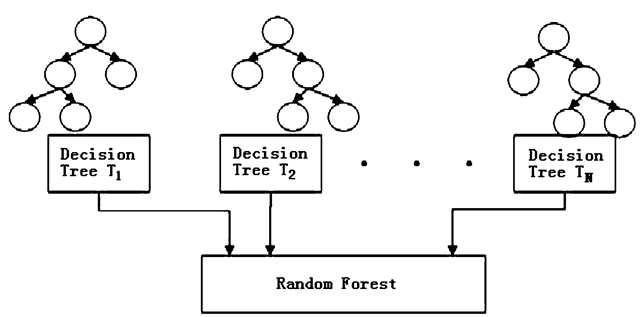
\includegraphics[width=0.8\linewidth]{images/rf}

A downside of both the CART and random forest algorithms (as well as many other algorithmic modeling approaches) is an inability to clearly quantify the roles played by individual variables in making predictions. However, the importance of individual variables in a random forest can still be expressed using a measure known as variable importance.

The random forest algorithm requires the following tuning parameters be specified in order to run:

\begin{itemize}
\tightlist
\item
  \texttt{ntree} - the number of bagged samples, \(\boldsymbol{B}\), onto which trees will be grown
\item
  \texttt{mtry} - the number of variables that are randomly chosen to be candidates at each split
\item
  Some sort of stopping criteria for individual trees, this can be:

  \begin{itemize}
  \tightlist
  \item
    \texttt{nodesize}, which sets the minimum size of terminal nodes

    \begin{itemize}
    \tightlist
    \item
      larger \texttt{nodesize} leads to shallower trees
    \item
      smaller node size allows for deeper, more complex trees
    \end{itemize}
  \item
    \texttt{maxnodes}, which sets the maximum number of terminal nodes an individual tree can have.
  \end{itemize}
\end{itemize}

\textbf{Applications of Random Forest}

Some of the applications of Random Forest Algorithm are listed below:

\begin{itemize}
\tightlist
\item
  Banking: It predicts a loan applicant's solvency. This helps lending institutions make a good decision on whether to give the customer loan or not. They are also being used to detect fraudsters.
\item
  Health Care: Health professionals use random forest systems to diagnose patients. Patients are diagnosed by assessing their previous medical history. Past medical records are reviewed to establish the proper dosage for the patients.
\item
  Stock Market: Financial analysts use it to identify potential markets for stocks. It also enables them to remember the behaviour of stocks.
\item
  E-Commerce: Through this system, e-commerce vendors can predict the preference of customers based on past consumption behaviour.
\end{itemize}

\textbf{When to Avoid Using Random Forests?}

Random Forests Algorithms are not ideal in the following situations:

\begin{itemize}
\tightlist
\item
  Extrapolation: Random Forest regression is not ideal in the extrapolation of data. Unlike linear regression, which uses existing observations to estimate values beyond the observation range.
\item
  Sparse Data: Random Forest does not produce good results when the data is sparse. In this case, the subject of features and bootstrapped sample will have an invariant space. This will lead to unproductive spills, which will affect the outcome.
\end{itemize}

\textbf{FAQ}

Q: Is RF a linear or non-linear model?\\
A: RF can capture complex, non-linear relationships.

Q: Is RF sensitive to Imbalanced Data?\\
A: Yes. It may perform poorly if the dataset is highly imbalanced like one class is significantly more frequent than another.

Q: What is the loss function?\\
A: Entropy/gini or any other loss function you want.

Q: Difference btw RF and a linear model?\\
A: A major difference is that a decision tree does not have ``parameters'', whereas the linear models need to create a functional form and find the optimal parameters.

\begin{center}\rule{0.5\linewidth}{0.5pt}\end{center}

\subsection*{Implementation in R}\label{implementation-in-r}
\addcontentsline{toc}{subsection}{Implementation in R}

\texttt{ranger} package offers a computation efficient function for RF.

\begin{Shaded}
\begin{Highlighting}[]
\NormalTok{RF\_ranger }\OtherTok{\textless{}{-}} \FunctionTok{ranger}\NormalTok{(}\AttributeTok{formula =}\NormalTok{ formula, }
                    \AttributeTok{data =}\NormalTok{ data\_before[idx,], }
                    \AttributeTok{probability =} \ConstantTok{TRUE}\NormalTok{,}
                    \AttributeTok{importance =} \StringTok{"permutation"}\NormalTok{, }
                    \AttributeTok{scale.permutation.importance =} \ConstantTok{TRUE}\NormalTok{,}
\NormalTok{                    )}
    \CommentTok{\# print(RF\_ranger)}
    
\NormalTok{rf.pred.test }\OtherTok{\textless{}{-}} \FunctionTok{predict}\NormalTok{(RF\_ranger, }\AttributeTok{data=}\NormalTok{data\_before[}\SpecialCharTok{{-}}\NormalTok{idx,])}\SpecialCharTok{$}\NormalTok{predictions}
\end{Highlighting}
\end{Shaded}

Parameters controlling the general process of RF:

\begin{itemize}
\tightlist
\item
  \texttt{probability=FALSE}: Whether to forecast a probability forest.
\end{itemize}

The hyperparameters \texttt{mtry}, \texttt{min.node.size} and \texttt{sample.fraction} determine the degree of randomness, and should be tuned.

\begin{itemize}
\tightlist
\item
  \texttt{mtry=500}: Number of variables to possibly split at in each node in one tree. In plain language, it indicates how many predictor variables should be used in each tree.

  \begin{itemize}
  \tightlist
  \item
    Default is the (rounded down) square root of the number variables. Alternatively, a single argument function returning an integer, given the number of independent variables.
  \item
    Range btw 1 to the number of predictors.
  \item
    If all predictors are used, then this corresponds in fact to bagging.
  \end{itemize}
\item
  \texttt{min.node.size}: The number of observations a terminal node should at least have.

  \begin{itemize}
  \tightlist
  \item
    Default 1 for classification, 5 for regression, 3 for survival, and 10 for probability. For classification, this can be a vector of class-specific values.
  \item
    Range between 1 and 10
  \end{itemize}
\item
  \texttt{sample.fraction}: Fraction of observations to be used in each tree. Default is 1 for sampling with replacement and 0.632 for sampling without replacement. For classification, this can be a vector of class-specific values.

  \begin{itemize}
  \tightlist
  \item
    Smaller fractions lead to greater diversity, and thus less correlated trees which often is desirable.
  \item
    Range between 0.2 and 0.9
  \end{itemize}
\end{itemize}

Parameters controlling what and how intermediate results are saved:

\begin{itemize}
\item
  \texttt{keep.inbag\ =\ FALSE}: Whether to save how often observations are in-bag in each tree.

  Set to \texttt{TRUE} if you want to check sample composition in each tree.
\item
  \texttt{importance\ =\ \textquotesingle{}none\textquotesingle{}\textbar{}\textquotesingle{}impurity\textquotesingle{}\textbar{}\textquotesingle{}impurity\_corrected\textquotesingle{}\textbar{}\textquotesingle{}permutation\textquotesingle{}}: Variable importance mode.
\item
  \texttt{scale.permutation.importance\ =\ FALSE}: Whether to scale permutation importance by standard error as in (Breiman 2001). Only applicable if \texttt{\textquotesingle{}permutation\textquotesingle{}} variable importance mode selected.
\item
  \texttt{write.forest\ =\ TRUE}: Whether to save \texttt{ranger.forest} object, required for prediction. Set to \texttt{FALSE} to reduce memory usage if no prediction intended.

  \begin{itemize}
  \tightlist
  \item
    Set to \texttt{FALSE} when you do parameter tuning.
  \end{itemize}
\end{itemize}

Q: How to tune hyperparameters?\\
A: Check out \href{https://mlr3.mlr-org.com}{\texttt{mlr3} package}. \href{https://r.geocompx.org/eco.html}{Here} is an example.

\begin{center}\rule{0.5\linewidth}{0.5pt}\end{center}

\subsection*{Imbalance Classification}\label{imbalance-classification}
\addcontentsline{toc}{subsection}{Imbalance Classification}

You can balance your random forests using case weights. Here's a simple example:

\begin{Shaded}
\begin{Highlighting}[]
\FunctionTok{library}\NormalTok{(ranger)}

\CommentTok{\# Make a dataste}
\FunctionTok{set.seed}\NormalTok{(}\DecValTok{43}\NormalTok{)}
\NormalTok{nrow }\OtherTok{\textless{}{-}} \DecValTok{1000}
\NormalTok{ncol }\OtherTok{\textless{}{-}} \DecValTok{10}
\NormalTok{X }\OtherTok{\textless{}{-}} \FunctionTok{matrix}\NormalTok{(}\FunctionTok{rnorm}\NormalTok{(nrow }\SpecialCharTok{*}\NormalTok{ ncol), }\AttributeTok{ncol=}\NormalTok{ncol)}
\NormalTok{CF }\OtherTok{\textless{}{-}} \FunctionTok{rnorm}\NormalTok{(ncol)}
\NormalTok{Y }\OtherTok{\textless{}{-}}\NormalTok{ (X }\SpecialCharTok{\%*\%}\NormalTok{ CF }\SpecialCharTok{+} \FunctionTok{rnorm}\NormalTok{(nrow))[,}\DecValTok{1}\NormalTok{]}
\NormalTok{Y }\OtherTok{\textless{}{-}} \FunctionTok{as.integer}\NormalTok{(Y }\SpecialCharTok{\textgreater{}} \FunctionTok{quantile}\NormalTok{(Y, }\FloatTok{0.90}\NormalTok{))}
\FunctionTok{table}\NormalTok{(Y)}

\CommentTok{\# Compute weights to balance the RF}
\NormalTok{w }\OtherTok{\textless{}{-}} \DecValTok{1}\SpecialCharTok{/}\FunctionTok{table}\NormalTok{(Y)}
\NormalTok{w }\OtherTok{\textless{}{-}}\NormalTok{ w}\SpecialCharTok{/}\FunctionTok{sum}\NormalTok{(w)}
\NormalTok{weights }\OtherTok{\textless{}{-}} \FunctionTok{rep}\NormalTok{(}\DecValTok{0}\NormalTok{, nrow)}
\NormalTok{weights[Y }\SpecialCharTok{==} \DecValTok{0}\NormalTok{] }\OtherTok{\textless{}{-}}\NormalTok{ w[}\StringTok{\textquotesingle{}0\textquotesingle{}}\NormalTok{]}
\NormalTok{weights[Y }\SpecialCharTok{==} \DecValTok{1}\NormalTok{] }\OtherTok{\textless{}{-}}\NormalTok{ w[}\StringTok{\textquotesingle{}1\textquotesingle{}}\NormalTok{]}
\FunctionTok{table}\NormalTok{(weights, Y)}

\CommentTok{\# Fit the RF}
\NormalTok{data }\OtherTok{\textless{}{-}} \FunctionTok{data.frame}\NormalTok{(}\AttributeTok{Y=}\FunctionTok{factor}\NormalTok{(}\FunctionTok{ifelse}\NormalTok{(Y}\SpecialCharTok{==}\DecValTok{0}\NormalTok{, }\StringTok{\textquotesingle{}no\textquotesingle{}}\NormalTok{, }\StringTok{\textquotesingle{}yes\textquotesingle{}}\NormalTok{)), X)}
\NormalTok{model }\OtherTok{\textless{}{-}} \FunctionTok{ranger}\NormalTok{(Y}\SpecialCharTok{\textasciitilde{}}\NormalTok{., data, }\AttributeTok{case.weights=}\NormalTok{weights)}
\FunctionTok{print}\NormalTok{(model)}
\end{Highlighting}
\end{Shaded}

Code Source: \url{https://stats.stackexchange.com/a/287849}

Fixed proportion sampling: \url{https://github.com/imbs-hl/ranger/issues/167}

\begin{center}\rule{0.5\linewidth}{0.5pt}\end{center}

\textbf{References}:

\url{https://remiller1450.github.io/m257s21/Lab10_Other_Models.html}

\section{Neural Network}\label{neural-network}

Neural networks are made up objects called ``layers'' and ``neurons'' and these things connect to each other in a specific way. Each layer has some number of neurons. For example, the first layer might have 10 neurons, the second might have 15, and so on. The number of layers and the number of neurons in each layer is a ``hyperparameter'', the user picks how many of each. Let's take a look at a single neuron.

\[
v_3^{(1)} = g(\boldsymbol{w}_3^{(1)}\boldsymbol{x} + b_3^{(1)})
\]

\begin{itemize}
\item
  The LHS, \(v_3^{(1)}\), will be the output. The superscript \((1)\) refers to the layer number; the subscript \(3\) refers to the neuron.

  An output here means just a single number. If we have say 15 neurons (subscript) for this first layer (superscript), then we will have 15 numbers come out of this first layer: \(\boldsymbol{v^{(1)}} = \{v^{(1)}_{1}, v^{(1)}_{1}, ..., v^{(1)}_{15}\}\) where the bolded \(v\) means a vector.
\item
  \(\boldsymbol{x}\) is our input vector.
\item
  \(\boldsymbol{w}\) is the weight/coefficient vector.
\item
  \(b\) is a bias or the intercept term, shifting the value of \(\boldsymbol{w}\cdot\boldsymbol{x}\) up or down.
\item
  \(g\) refers to a ``non-linear'' function, often called as the ``activation function''.
\end{itemize}

  \bibliography{book.bib,packages.bib}

\end{document}
